%------------------------------------------------------------
% thesis - Andy Taylor 
%------------------------------------------------------------
\documentclass[11pt,a4paper,titlepage,twoside,openrigh]{book}
\usepackage{style/uomthesis}  % Unimelb thesis template
%---------------------------
% formats and definitions
%---------------------------
%\newcommand{\markblankpages}{}     % option:"This page intentionally left blank."
\newcommand{\archivalpapernote}{}  % option: copy submitted to the library
%% add DRAFT water mark
\usepackage{draftwatermark}
\SetWatermarkText{DRAFT} 
\SetWatermarkLightness{0.98}
\SetWatermarkAngle{45}
\SetWatermarkScale{1.2}
   % draft watermark
%-----------------------------------
% Packages
%-----------------------------------
\usepackage{setspace}
\onehalfspacing
\usepackage{natbib}
\usepackage{enumerate}
\usepackage{subcaption}
\usepackage{float}
\usepackage{paralist}
\usepackage{amssymb}
\usepackage{amsmath}
\usepackage{amsthm}
\usepackage[mathscr]{eucal}
\usepackage{graphicx}
\usepackage[hidelinks]{hyperref}
%-----------------------------------
% figure size defaults
%-----------------------------------
\newlength{\myfigwidth}
\setlength{\myfigwidth}{400pt}
%-----------------------------------
% References
%-----------------------------------
\bibliographystyle{bib/ametsoc2014}
%------------------------------------------------------------------------
% colours & symbols
%------------------------------------------------------------------------
\usepackage[framemethod=tikz]{mdframed}
\usepackage{color}
\definecolor{mygrey}{rgb}{0.9,0.9,0.9}
\definecolor{mygreen}{rgb}{0,.4,0}
\usepackage{listings}
\lstset{
language=bash,                   % Code langugage
backgroundcolor=\color{mygrey},  % choose the background color; you must add \usepackage{color} or \usepackage{xcolor}
basicstyle=\ttfamily,            % Code font, Examples: \footnotesize, \ttfamily
commentstyle=\color{mygreen},    % comment style
breaklines=true,
}
% bullet symbol
\renewcommand{\labelitemi}{{\tiny$\blacksquare$}}
% highlights
\newcommand{\BoxBegin}{\begin{mdframed}[hidealllines=true,backgroundcolor=yellow!30]}
\newcommand{\BoxEnd}{\end{mdframed}}

% matrices etc
\newcommand{\M}[1]{\mathsf{#1}}
\newcommand{\V}[1]{\mathbf{#1}}

%-----------------------------------
% config
%-----------------------------------
% no indents
\setlength\parindent{0pt}
% Allow equations to break over pages...
\interdisplaylinepenalty=2500
% Command to stop equation breaks
% Note: enclose this in braces when used...
\newcommand{\donotsplitoverpages}{\interdisplaylinepenalty=10000}               

%\newcommand{\figureInit}{\begin{figure}[h]\centering}
%------------------------------------------------------------------------ 
% shortcut text
%------------------------------------------------------------------------ 
\newcommand{\TITLE}{`TITLE'}
\newcommand{\ALTTITLE}{`ALT TITLE'}
\newcommand{\BOM}{Australian Bureau of Meteorology}
\newcommand{\LTE}{\textbf{\texttt{LTE}}}
\newcommand{\ATGF}{\textbf{\texttt{ATGF}}}
\newcommand{\ATGP}{\textbf{\texttt{ATGP}}}
\newcommand{\SSH}{\textbf{\texttt{ssh}}}
\newcommand{\BL}{\textbf{\texttt{Bluelink-OceanMAPS}}}
\newcommand{\MOM}{\textbf{\texttt{MOM}}}
\newcommand{\ROMS}{\textbf{\texttt{ROMS}}}
\newcommand{\GODAE}{\textbf{\texttt{GODAE}}}
\newcommand{\OGCM}{\textbf{\texttt{{OGCM}}}}       %{\textbf{\texttt{OGCM}}}
\newcommand{\OFAM}{\textbf{\texttt{{OFAM}}}}
\newcommand{\OFAMHR}{\textbf{\texttt{{OFAMHR}}}}
\newcommand{\NWP}{\textbf{\texttt{NWP}}}
\newcommand{\OTIS}{\textbf{\texttt{OTIS}}}
\newcommand{\GOOS}{\textbf{\texttt{GOOS}}}
\newcommand{\obc}{\textbf{\texttt{obc}}}
\newcommand{\ANTT}{\textbf{\texttt{ANTT}}}
\newcommand{\CTE}{\textbf{\texttt{CTE}}}
\newcommand{\SAL}{\textbf{\texttt{SAL}}}
\newcommand{\AG}{\textbf{\texttt{ACCESS-G}}}
\newcommand{\AR}{\textbf{\texttt{ACCESS-R}}}
\newcommand{\ER}{\textbf{\texttt{eReefs}}}
            
%---------------------------
% metadata
%---------------------------
\title{Sea level forecasts, tide prediction and mesoscale operational oceanography in Australia}
\author{Andy Taylor}
\orcid{0000-0003-1258-5002}
\submissionmonth{Dec}
\submissionyear{2021}
\department{School of Earth Sciences}
\university{\textsc The University of Melbourne}
%----------------------------------------
\begin{document}
    %---------------------------
    % front 
    %---------------------------
	\begin{frontmatter}
		\frontmatterheadings    % collect information for title page        
		\maketitle              % title         
		\makedeclaration        % author declaration
		
\begin{abstract}
This is the abstract
\end{abstract}
\clearpage

		
% Optional preface to the dissertation
\begin{preface}

This thesis with publication is built around the following peer-reviewed publications:

\vspace{5mm}
\hangindent=3em
\hangafter=1
Taylor, A. J. and Brassington, G. Sea Level Forecasts Aggregated from Established Operational Systems. Journal of Marine Science and Engineering 5, 33 (2017).

%\citep{Taylor:2017coa}


\vspace{5mm}
\hangindent=3em
\hangafter=1
Taylor, A. J. and Brassington, G. B. Sea Level Anomaly Forecasts on a Coastal Waveguide. Weather and Forecasting 35, 757–770 (2020).
%\citep{Taylor:2020}

\vspace{5mm}
\hangindent=3em
\hangafter=1
Extension material from the later presented at:
\vspace{5mm}
\hangindent=3em
\hangafter=1

Taylor, A., Greenslade, D., Zhou, X., and Brassington, G. (2020). National NonTidal Sea Level Forecasts on a Coastal Waveguide. Coastal Engineering Proceedings, (36v), currents.26. https://doi.org/10.9753/icce.v36v.currents.26
%\cite{10.9753/icce.v36v.currents.26}

\vspace{5mm}
\hangindent=3em
\hangafter=1
The material comprising chapter \ref{chp:tideFlavours} is in preparation for stand-alone publication.

\vspace{5mm}
\noindent  All funding and in-kind support for this research provided by the Australian Bureau of Meteorology. 

\end{preface}


		
\begin{acknowledgements}

% stop indents
{\parindent0pt

First and foremost I acknowledge the traditional ownership of the lands and seas that host Australia. These coasts have been known for so long.
\newline{}

Thanks to the ever-fantastic Kulja and our wanderings over mudflats and mangroves that first put the tides under my feet.   
    %Wetland people ..Pelican
    
%\newline{}    
    
Big thinks to Gary Brassington at the Bureau of Meteorology for making this whole effort possible.

%\newline{}

Tides  unit - James, Bill and Mike
Forecasters - James Taylor, Ben Hague and more
Phil Shinkfield , Jane Warne and more
Diana
    
The wider Bluelink community
David Griffin, Paul Sandery    
    
Unimelb
Kevin Walsh

OS early input 
Mike Foreman
Ed Zaron
%Lana and Gary E

%%%%%%%%%%%%%%%%%%%%%%%%%%%%%%%%%%%%%%%%%%
%\newline{}

Observational data shared with the Bureau from external agencies was important for this study, in particular from:
\begin{itemize}
    \item Manly Hydraulics Laboratory \url{http://mhl.nsw.gov.au/}
    \item Queensland Government Department of Environment, Land and Water \url{https://www.qld.gov.au/environment/coasts-waterways/beach/storm-sites]}
\end{itemize}


% template from git bloke	
And thanks for the LaTeX template \url{http://jpap.org/projects.html} by John Papandriopoulos.

}   % end no indent
\end{acknowledgements}

		{
			\singlespacing
			\tableofcontents
			\listoffigures
			%\listoftables   % not for less than 10 tables
		   \clearpage
		}
   \end{frontmatter}
    %----------------------------------------------
	% main
    %--------------------------------------------
	\begin{mainmatter}
		\mainmatterheadings
		
\chapter{Introduction}
%=========================================================================
Dig this

%========================
\section{Aims and Objectives}\label{s:aims}


\subsection{Do this}

Content here:
% \begin{figure}
%     \centering
%     \begin{subfigure}[c]{0.617\textwidth}
%         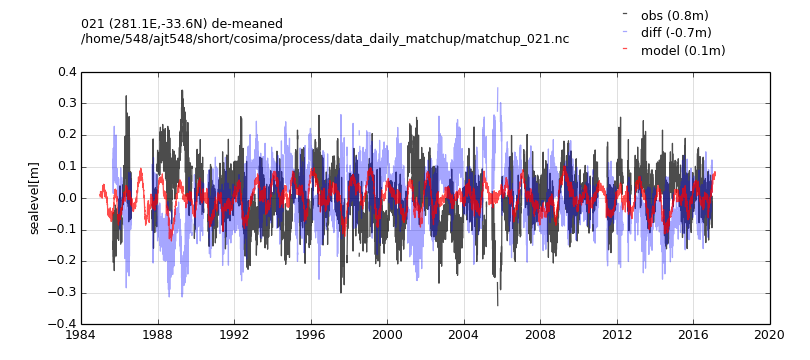
\includegraphics[width=\textwidth]{figures/plot.png}
%     \end{subfigure}\qquad
%     \begin{subfigure}[c]{0.289\textwidth}
%         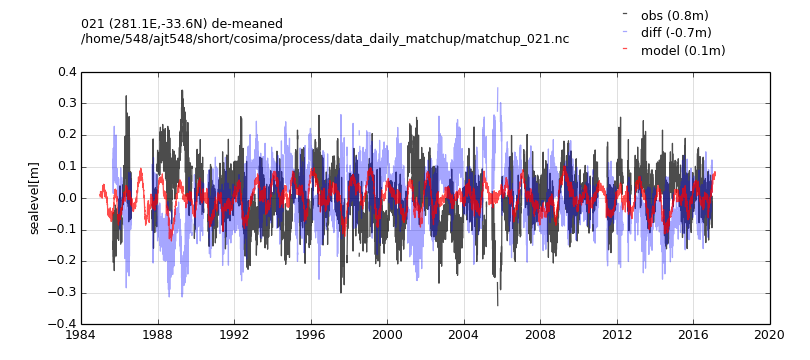
\includegraphics[width=\textwidth]{figures/plot.png}
%     \end{subfigure}\qquad
%     \vspace{2ex}
% \end{figure}
\section{Thesis Plan}\label{s:thesisplan}


		\chapter{Sea level forecasting concepts}
\label{chp:forecastConcepts}
\section{Ocean tide prediction}
\label{sec:tidesOverview}
%-----------------%
\begin{quote}
Tidal prediction is the oldest form of ocean prediction, and is still the most accurate \citep{Parker:2007wq}. 
\end{quote}
%-----------------%
\subsection{Why it is worth unpacking ocean tides}
\label{sec:semantics}
The topic of ocean tides is particularly rich in ambiguous and arcane terminology.  
Moreover, it is apparent that this terminology and the underlying concepts lead to miscommunication within operational forecasting.  And as operational centres like the Bureau of Meteorology increasingly bring these conventional tidal concepts into the same setting as geophysically `concrete' simulations (introduced in section \ref{sec:concrete}) the need for clarity is amplified.  This potential for confusion is motivates the following exposition of relevant concepts built into the practices of ocean tide prediction.
\newline{}


Tidal methods of analysing and forecasting the ocean have a long legacy in the history of western science.  Economically significant tidal sea level predictions in fact pre-date the whole modern scientific enterprise, and the evolution of the tidal perspective mirrors much of the story of classical continuum physics.

The \cite{Cartwright:2000tt} telling of the history of ocean tide science is illustrative. Remarkably, and perhaps typically, this scientific history of tides never even attempts to pin down a definition of what tide really should mean.  This surely deliberate exclusion stands in stark contrast to the minutiae of historical approaches and formulations and that the history covers.  The absence of definition may be read as an assertion that the \emph{history itself} is the only meaningful way to frame the scope of tidal science.
\cite{Pugh:1996uz} at least addresses the question of definition explicitly and in doing so casts a very wide net that catches almost anything that can be considered periodic.
\begin{quote}
Although any definition of tides will be somewhat arbitrary, it must emphasize this periodic and regular nature of the motion, whether that motion be of the sea surface level, currents, atmospheric pressure or earth movements. We define tides as periodic movements which are directly related in amplitude and phase to some periodic geophysical force \ldots.
\end{quote}
It is notable that whilst for Pugh \emph{periodicity} is a key feature of anything that is `tidal', he does not lock this periodicity to astronomy.  Pugh's pragmatic definition appears to be designed to best accommodate the conventional methods of harmonic analysis and sea level prediction that are so well established in operational agencies. Whilst this periodicity-stressing definition sensibly reflects the context of Pugh's text, it is certainly not the only working conceptualisation of what constitutes ocean tides; either within the operational forecasting context or in academic settings. 

In contrast to the periodic definition, most modern authors place the tidal potential in a defining role. Such an emphasis on the tidal potential or Astronomical Tide Generating Forces \ATGP{} reflects a greater regard for dynamics and inputs, as opposed to observed outputs, that is more complimentary to the wider field of geophysical fluid dynamics.  
\cite{Hendershott:1981ub} treats ocean tides as that subset of oceanographic long waves driven by the \ATGP{}.  Notably his discussion is careful with the distinction between dynamics and `practical tide prediction'. But even Henderscott's primarily dynamical perspective is imbued with the cultural interplay of physics and pragmatic prediction; as illustrated by his inclusion of the rather aphysical radiational potential concept associated with the \cite{Munk:1966ts} response method tradition.
The Australian Tide Manual \cite{PCTMSL-sp9} similarly reflects the historical intertwining of tidal physics and practical prediction methods; such that any forcing physics simply provides a backdrop to the singular focus on harmonic prediction.   
A step removed from ocean prediction, \cite{10.1016/b978-0-444-53802-4.00058-0} provides a modern physical perspective that both emphasises the core role of the tidal forcing (in this case for earth tides) whilst adopting the well established terminology derived from the long history of ocean tide prediction. A similar emphasis on the physical forcing within the historical perspective is taken by \citep{Flinchem:2000kp} in a  discussion of analysis methods associated with non-stationarity in ocean tide patterns.
The centrality of \ATGP{} be the approach employed in the present work as well.


Further on semantic issues, it is worth highlighting the extent to which the subject of ocean tides raises ostensibly oxymoronic terminology.  
Geophysists can define an \emph{a-periodic} pole tide on the basis of the dynamic connection to gravitational body forces associated with astronomical motions.   And valid discussion of \emph{non-stationary} tides \cite{Ray:2011tj}, \emph{quasi-periodic} tidal phenomena \citep{Flinchem:2000kp} or \emph{storm} tides \cite{Horsburgh:2008gw} in the literature and operational products each conceptually clash with the perspective of conventional harmonic analysis.  
A comparable semantic disconnect can arise in circumstances where a tidal prediction exceeds the designated Highest Astronomical Tide.   
Each of these definitions are sensible in context, but can potentially be a source of miscommunication with the development and delivery of operational forecasts.    Chapter \ref{chp:tideFlavours} proposes measures to partially mitigate such problems.

%-----------------%
\subsection{Common foundation of the \ATGP{}}
Reference to the astronomical tide generating potential (\ATGP{}) is here considered to be the common foundation what is properly considered a tidal method or tidal phenomena.  
The \ATGP{} is an abstraction developed from positional astronomy and classical gravity theory alone.   Perhaps surprisingly for some readers, the underlying role of positional astronomy is formulated in an entirely geocentric, effectively pre-Copernican, framework. 
Figure \ref{fig:tideForceFlow} schematically illustrates the conceptual connections from positional astronomy, to the \ATGP{} and geophysics through to observed sea level .  
Differing treatment of the intermediate parts of this flow chart, the geophysical modelling, effectively comprise the alternative approaches to sea level forecasting.  Of special relevance to the present focus are the details of any decomposition of observed sea level into tidal and non-tidal categories.   The dotted lines connecting nominally non-tidal components indicate that the gravitationally forced response is not the sole factor in discussions of tidal sea level. 
%-----------------
\begin{figure}[h]
    \begin{center}
    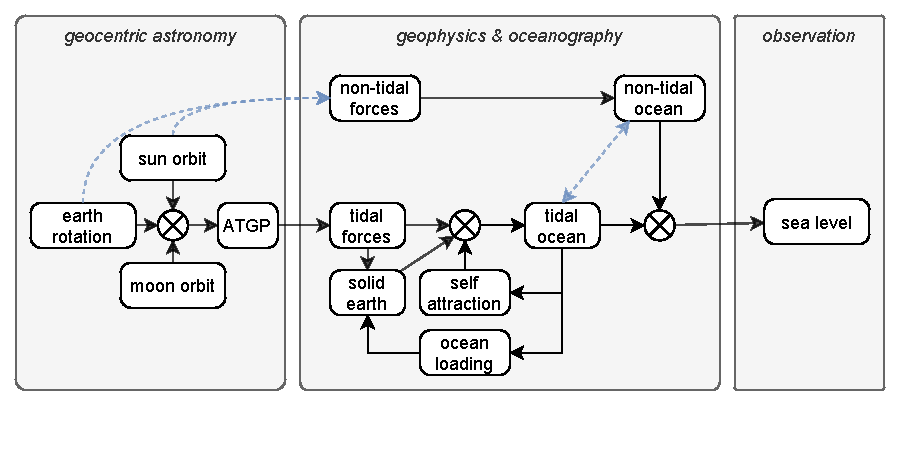
\includegraphics[width=\figwidthFull]{figures/diagrams/tidal_force_flowchart.pdf}
    \caption{Ocean tide flow chart (following Agnew \citep{Agnew:2011ub}.  Reference to the \ATGP{} is common to tidal analysis and prediction methods, whilst the treatment of tidal/non-tidal connections can differ markedly.}
    \label{fig:tideForceFlow}
    \end{center}
\end{figure}
%-----------------
Before expanding on the role of the tidal forcing, the recent work of \cite{10.1016/j.oceaneng.2020.107013} is worth mentioning.   Regardless of the finer details, this observation-based machine learning application to tide prediction is still founded on the connection between positional astronomy and sea level, but simply makes the connection more indirect by relying on easily accessible moon phase data.
%-----------------i
\subsection{Basic development of the \ATGP{}}  \label{sec:basic_potential}
The centrality of the tidal generating potential to sea level forecasting warrants further elaboration, in order to later explicate the manner in which conventional and dynamic sea level forecasts respectively represent tides. 

The \ATGP{} is a mathematical abstraction founded on a consideration of the classical gravitational field near the Earth surface. The temporal variations of gravity in the vicinity of this surface are developed as a function of the \emph{geocentric} relative positions of the celestial bodies.
For ocean tide applications, only the two celestial bodies, the moon and sun, are considered relevant on the basis of relative contribution to the perceived gravity field changes. It follows that the information required for computation of this lunisolar tidal potential is encapsulated in the celestial positions (ie ephemeris) of the moon and sun alone \citep{Agnew:2011ub}.


The full gravity field is defined as a scalar potential in space fulfilling the Laplace equation $\Delta V=0$ \citep[sec 5.3.1]{Urban:2013vl}.  The spatial field $V(\theta,\lambda,r)$ can be formulated in spherical geocentric (ie fixed earth) coordinates as a weighted sum of surface spherical harmonics. As a potential field, contributions from each mass element can be computed separately and linearly superposed.

The specific subset of $V$ attributed to the celestial bodies external to the Earth, but excluding components acting uniformly over the Earth's surface, is defined to be the tidal potential \ATGP{} or $V_T$.
The associated tidal acceleration at any particular point on the earth surface can also be thought as the vector difference between the direct attraction of each celestial body and the orbital acceleration about the Earth-Body barycenter \citep{Wenzel:1997kn}.


The subset $V_T$ of $V$ that is relevant to ocean dynamics is formulated in geocentric coordinates following the convention of \cite{Cartwright:1973em} hereafter \CTE{}, and more recent notation of \cite{Desai:2006wo}:
\begin{equation}
    \eta_{eq} = \frac{V_T(t,\theta,\lambda) }{g} = \sum_{n=2}^{\infty} \sum_{m=0}^{m=n} M_{nm} P_{nm}( \sin(\theta) ) \text{Re} \left [ c^{*}_{nm}(t) e^{im\lambda} \right ]
    \label{eq:VT}
\end{equation}
Where the potential is described only on an idealised spherical earth surface in terms of time, longitude $\lambda$ and latitude $\theta$, as a sum of functions described further below. 

$P_{nm}$ are the associated Legendre polynomials of degree $n$ and order $m$.  Writing $P_{nm}(\sin(\theta))$ gives the surface spherical harmonics.  The fact that the sum begins at $n=2$ is discussed below.
$M_{nm}$ are normalisation factors, that whilst not of direct interest here are noted to follow different conventions between applications \citep{IERS2003}.
Figure \ref{fig:VTmaps} provides a visualisation of the field and a decomposition into spherical harmonics a single snapshot in time.
%-------------------------------
\begin{figure}[h]
    \begin{center}
    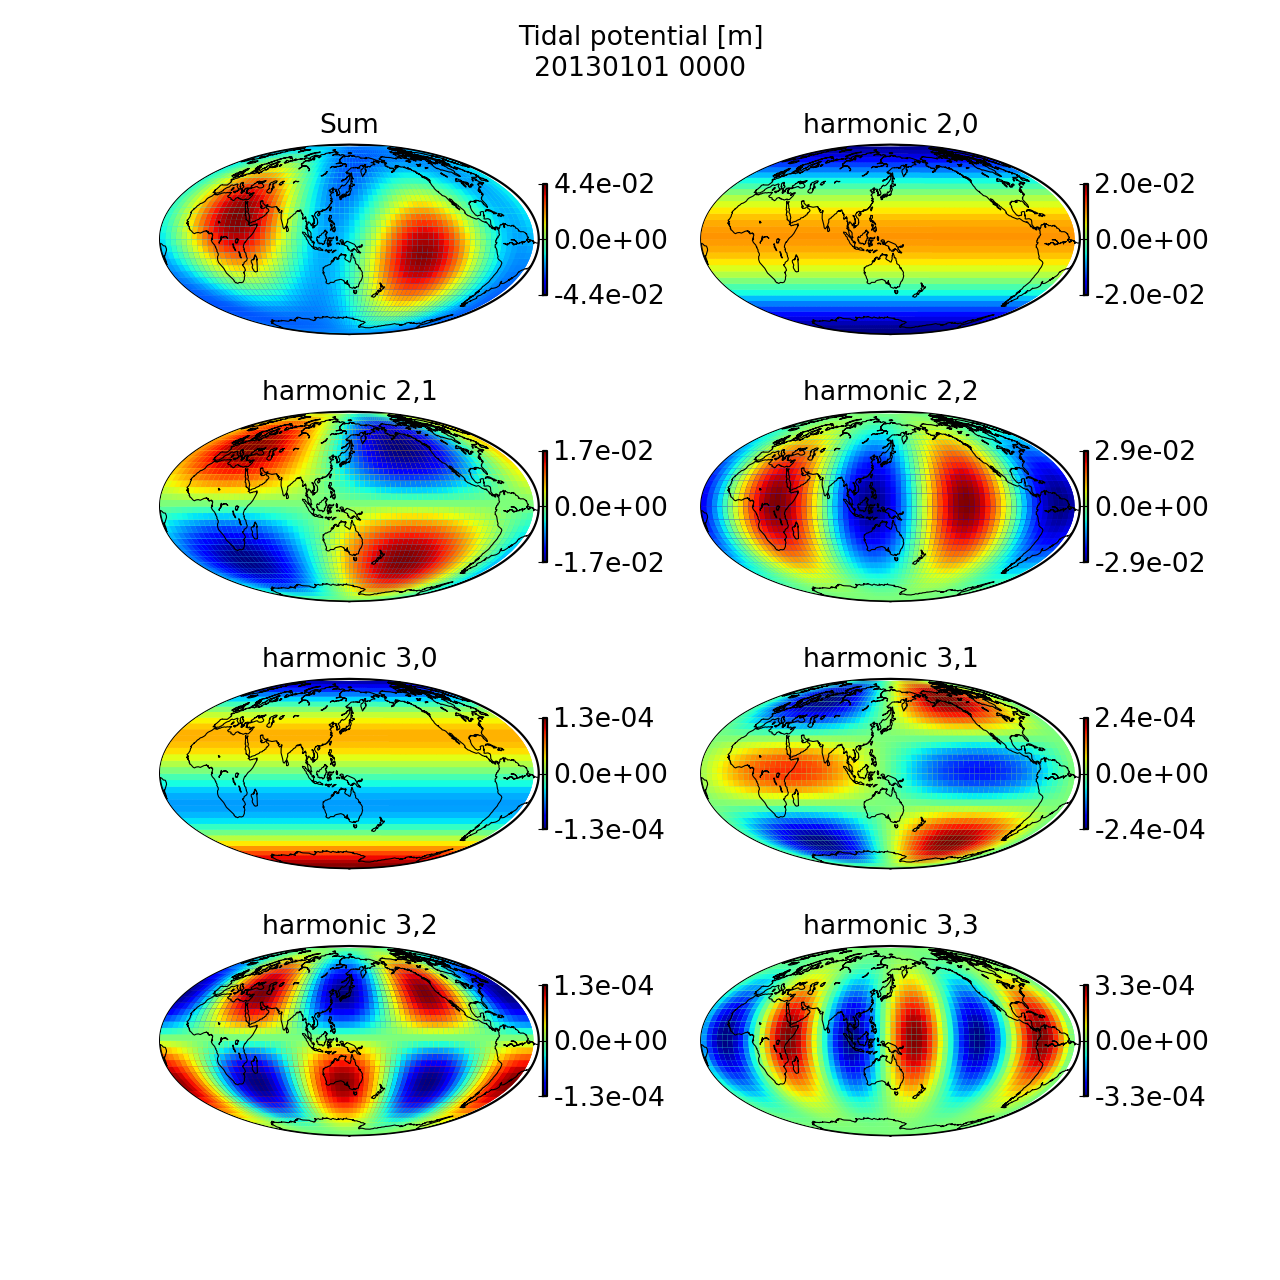
\includegraphics[width=\figwidthBig]{figures/maps/tidal_potential_spatial_20130101_0000.png}
    \caption{Snapshot of global $\eta_{eq}$ field illustrating spatial decomposition into spherical harmonics.  Note the wide variation of relative magnitude. When comparing to formulations recall that those decompositions are per body; ie an independent set for the moon and sun. }
    \label{fig:VTmaps}
    \end{center}
\end{figure}
%-------------------------------
Equation \ref{eq:VT} and the visualisation in \ref{fig:VTmaps} quantify the potential $V_T$ normalised by the standard value for Earth gravity $g$; a quantity defined as the \emph{equilibrium tide} $\eta_{eq}$.  
A convenience of normalising the potential field as $\eta_{eq}$ is that the quantity has units of height. But this formulation unfortunately invites confusion with actual ocean elevations; whereas the equilibrium tide really only has a very abstract and indirect connection to observed ocean tide heights.
Specifically, whilst useful for formulating the driving force, the any direct connection to ocean response is only via the thought experiment of a shallow water idealisation of boundary-free ocean with ``no dynamic effects'' as stated by \cite[Eq 9.8.3]{gill1982atmosphere}; that is, the equilibrium tide is a useless approximation to ocean heights at all expect the longest periods \cite{Egbert:2003jd}.


Equation \ref{eq:VT} represents the spatial decomposition of a surface potential field over the globe.  Of itself, such a formulation asserts nothing specific about the causation of the field.  It embodies no astronomy or ocean dynamics.
Practical implementation of \ref{eq:VT} requires choices regarding the set of harmonics $(n,m)$ to be included and the determination of the time varying complex weights $c_{nm}(t)$.


Only a small set of $(n,m)$ is taken to be relevant for ocean tidal dynamics; in contrast to the thousands of terms utilised for some earth gravity studies. What counts as a relevant ocean subset is generally determined on the basis of the relative magnitude of the terms and the nature of the temporal variation in geographic coordinates.

It is only the horizontal gradient of the potential $\nabla V_T$ that can drive changes in the distribution of ocean mass.   Which to be clear states that the effect of the \ATGP{} on the ocean is to slide mass side-to-side, not directly pull it up.   And furthermore, only \emph{temporal} changes in this horizontal gradient will effect the non-static ocean distribution. Subsequently degrees $n=0,1$ are not relevant to ocean tides.   This is represented in equation \ref{eq:VT} by the lower limit $n=2$ of the outer sum.
For almost ocean tide applications an upper limit of $n=2$ is taken to be sufficient, or at most $n=3$; again in contrast to some earth gravity studies.  This choice is based on the rapid decline in relative magnitude of each harmonic with increasing $n$ for the luni-solar system - discussed below regarding equation \ref{eq:c}.



The zonal harmonics $(n,m) = (2,0)$ for each body are of particular relevance to the slower patterns of sea level.  Specifically, by having no variation in $\lambda$ these harmonics don't vary geographically with the daily rotation of the earth.   However, the slower changes in the declination of each body do drive an ocean mass response and is associated with the both the long period and permanent tides.  
What is considered to comprise the \emph{permanent} component of the tide potential is effectively time scale and application dependant and is an important detail for geodesy and gravity studies.  \cite[section 5.3.3.2]{Urban:2013vl}.  For ocean forecasting, the role and formulation of the permanent tide becomes relevant in the decomposition of mean sea level, and estimation of what constitutes dynamic ocean topography in a consistent geodetic reference framework \citep{Filmer:2018cu}\cite{10.1007/bf02520477}.


All of the temporal variation of $V_T$ is contained in the time series of complex scalar weights $c_{nm}(t)$.
It is significant that these temporal variations of the \ATGP{} for the entire globe can thus represented by a small number of scalar timeseries - a single complex timeseries for each spherical harmonic included.  For the typical set of harmonics used for ocean tides $(n,m)=(2,1),(2,2)$ this represents a significant compression of spatial information.  
Given the positions in the geocentric reference frame $\theta,\lambda,r$ for both moon and sun, the coefficients are:
\begin{align}
\label{eq:c}
c_{nm}(t) &= a_{nm}(t) + ib_{nm}(t) \nonumber \\
          &= \sum_{b=\text{moon},\text{sun}}    \frac{4 \pi GM_{b}}{g r_{b}}  \frac{(2-\delta_{m0})} {(2n+1)} \left(\frac{a}{r_b} \right)^n    M_{nm} P_{nm}( \sin(\theta_b) ) e^{im\lambda_b}
\end{align}
The normalisation used in the determination of $c_{nm}(t)$ must be consistent with that used for equation \ref{q:VT}.
Note that $\theta,\lambda$ in Equation \ref{eq:c} are equivalent to the geographic coordinates of the respective sub-body point at a given time. 
Where $\delta_m0 = 1$ for $m==0$ and $\delta_{m0} = 0$ for $m \neq 0$.\\
Normalisation $M$ is given by Equation \ref{E:M}. The radial scale $a$ is conventional taken as the semi-major axis from the ellipsoidal georeference. 
%---------------------
\begin{figure}[h]
\begin{center}
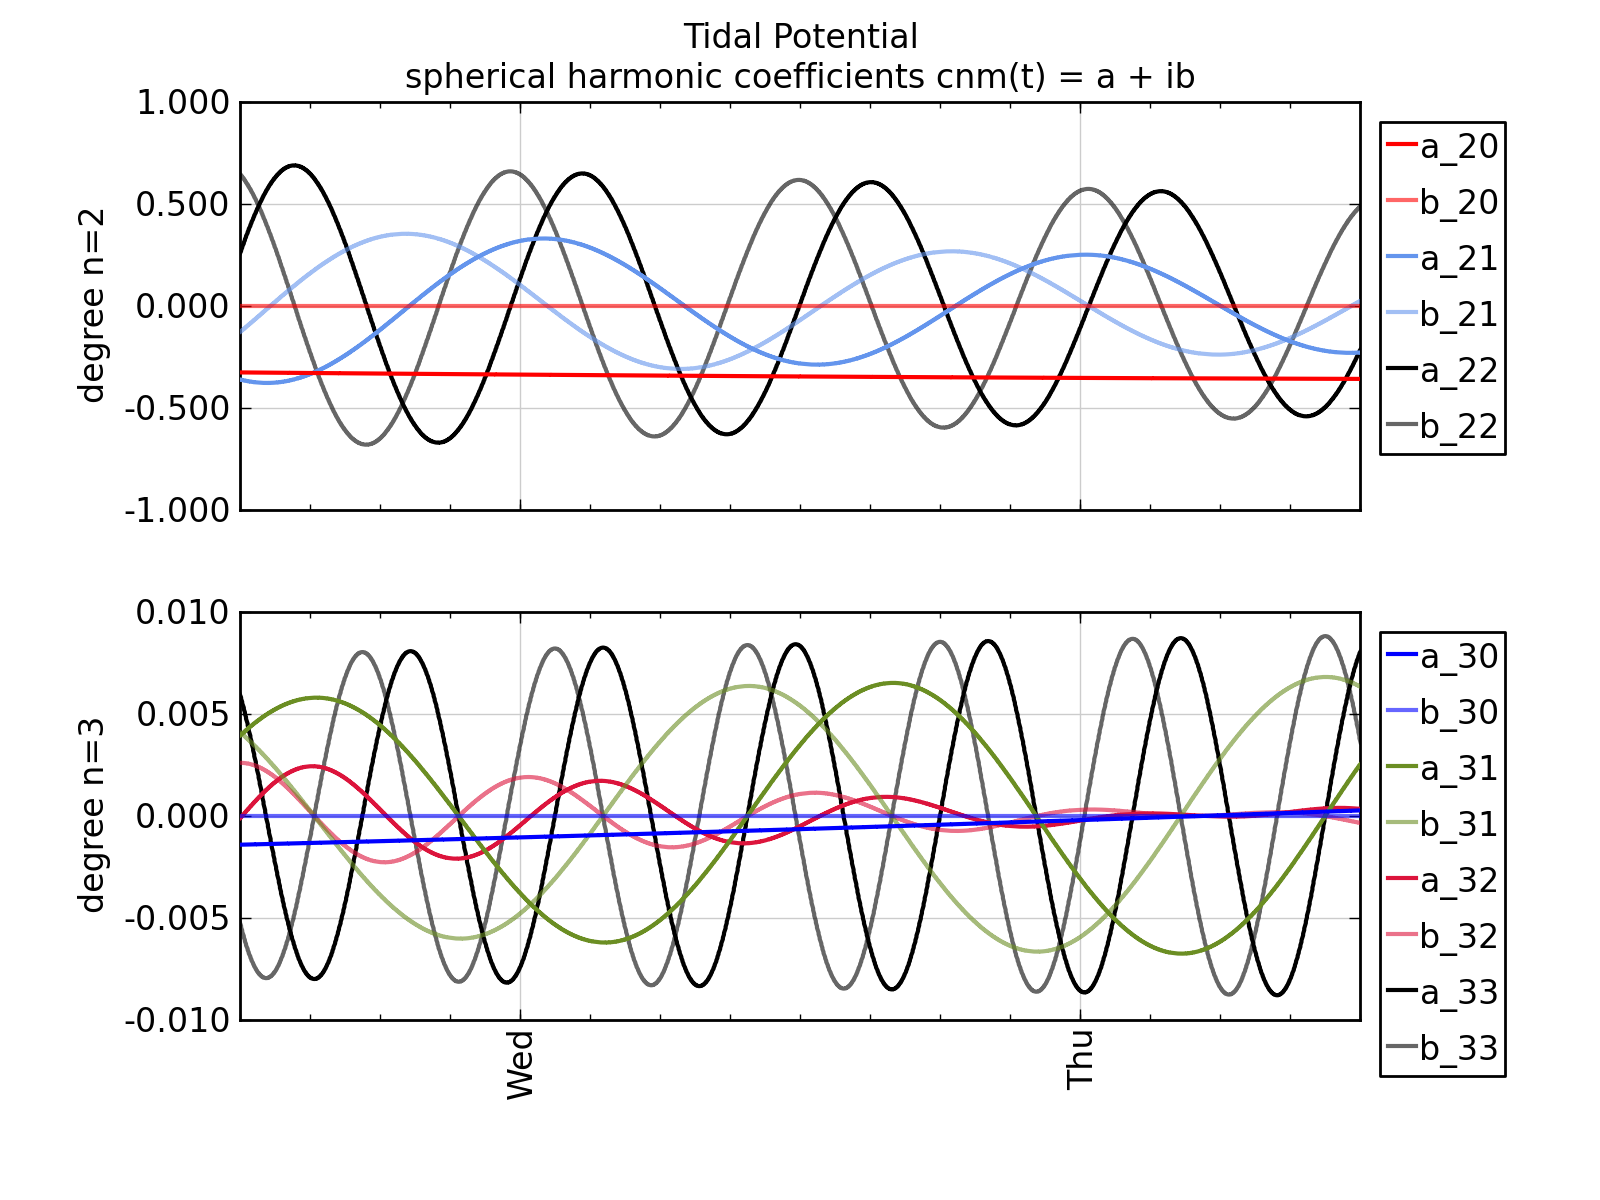
\includegraphics[width=\figwidthBig]{figures/plots/tidal_coeff_timeseries_2days.png}
\caption{Snapshot of time varying coefficients $c_{nm}(t)$.  In the upper panel, classification of $c_{2m}$ into long (red) , diurnal (blue) and semi-diurnal (black) species is evident.  Note the much smaller magnitude of higher degree harmonics.}
\end{center}
\end{figure}
%---------------------
The rapid decay of the scaling term $\left(\frac{a}{r_b} \right)^n$ with n is the basis for excluding higher degree harmonics from ocean tide applications.  In the case of the Moon, the magnitude of the $n=3$ potential field is more than 2 orders of magnitude smaller than $n=2$.  The associated force also decays, but not quite so rapidly due to the decreasing spatial length scales of the higher harmonics.  This decay is apparent in the colorbars of Figure \ref{fig:VTmaps}\\
The same relative magnitude argument is applied to neglecting more distant celestial masses from formulation of $\eta_{eq}$.

%-----------------%
\subsection{Primary role for temporal variations}
\label{sec:temporal}
The temporal variation of the \ATGP{} is of special relevance to ocean tide prediction.  And inspection of equation \ref{eq:VT} show that all of this variability is contained within the coefficients $c_{nm}(t)$.  
Any tidal method that applies $c_{nm}(t)$ from a numerical ephemeris in time-space could be said to be \emph{direct}. 
However, transformation of $c_{nm}(t)$ into frequency-space is in fact the basis of many tidal methods.   The highly clustered frequency content of $c_{nm}(t)$ renders this transformation particularly useful.  
Transformation of $c_{nm}(t)$ into frequency space is the basis for \underline{harmonic developments} of the \ATGP{}. Whilst there have been different approaches to performing this development, the common representation is given in Equation \ref{E:harmonic} following \citep{Desai:2006wo} and \citep[Eq 13]{Cartwright:1971iz}.
Furthermore, the ephemeris details for the celestial bodies can be modelled with relatively simple polynomial functions of time; discussed further below. 


It is this harmonic decomposition of the \ATGP{} that leads to the conventional ocean tide practice of harmonic analysis.
%----------------
\begin{equation}
    c_{nm}(t) = \sum_{k} H_{nmk} e^{-i( t\theta_{nmk})} = \sum_{k} H_{nmk} e^{-i( t\omega_{nmk} + \beta_{nmk})}
    \label{E:harmonic}
\end{equation}
%----------------
The index $k$ represents a discrete series of tidal components; potentially expanded out to hundreds of terms.  Each component is associated with a discrete point in complex frequency-space with amplitude $H$, frequency $\omega$ and phase $\beta$.

Despite a common misconception, it is important to emphasise that equation \ref{E:harmonic} does not represent a Fourier series.  The finite sequence of frequencies $\omega_{nmk}$ are derived from the relative motions of the earth-moon-sun system and do not provide either an orthogonal set of sinusoids nor a complete basis.

Despite not being orthogonal, the harmonic decomposition does provide a special list of frequencies that can be ranked by a scalar magnitude. 

\citet{Doodson:1921kt} introduced a novel and influential system of notation for specifying $\theta_{nmk}$ based on a laborious harmonic decomposition of $V_T$ using Brown's lunar theory; that is, a polynomial model for the lunar ephemeris.  
In the Doodson formulation, all the relevant astronomical information is summarised by code of 6 small integers; together called the Doodson number or argument numbers.   Each position in the code is associated with an fundamental astronomical concept as summarised in Table \ref{T:doodson}.  Doodson codes are in common use across the tidal literature and provide the only useful means of describing tidal components beyond the small number associated with traditional Darwin names such as M2, K1, O1, S2.
Of these traditional names \citet{10.1016/b978-0-444-53802-4.00058-0} correctly states that `` [whilst] it is convenient to have a shorthand way of referring to these harmonics; unfortunately, the standard names,  now totally entrenched, ... simply have to be learned as is.''.

There has been some variation of conventions with regard to the exact formulation of Doodson numbers.  One such detail is the avoidance of negative integers in the code by the addition of the arbitrary constant 5 to all integers except $d_1$.   A less common variation involves the use of solar-hour in place of lunar hour $\tau$.  
In essence the Doodson codes provide a compact unique specification, or in practice \emph{definition} of frequencies relevant to tidal methods.

Whereas the Doodson codes provide a reliable way to describe these tidal frequencies, the mapping to traditional names is unfortunately not always consistent and can lead to errors if transferring parameter data between software platforms; this issue is taken up in chapter \ref{chp:tideFlavours}.


\begin{table}[htp]
\caption{Doodson astronomical arguments.  Small integer combinations of these six numbers $d_1 d_2 d_3 d_4 d_5 d_6$ are used to classify tidal components.  Recall that longitudes are celestial, not geographic, coordinates}
\begin{center} 
\begin{tabular}{|c|c|c|}
\hline
Description                            & Argument          & Period\\
\hline
Mean lunar hour                        & $\tau$            & $\sim$ 1 day      \\
Moon mean longitude                    & $s$               & $\sim$ 27 days    \\  
Sun mean longitude                     & $h$               & $\sim$ 1 year     \\
Longitude of lunar perigee             & $p$               & $\sim$ 8.85 years \\
Negative longitude of mean lunar node  & $N^\prime$        & $\sim$ 18.6 years \\
Longitude of Sun mean perigee          & $p_1$             & $\sim$ 20000 years\\
\hline
\end{tabular} 
\end{center}
\label{T:doodson}
\end{table}


Equation \ref{E:doodson} gives the angular argument for a single tidal component $k$ as a function of the 6 astronomical arguments.   As discussed above, the astronomical arguments embody an analytical ephemeris for the Moon and Sun rather than a direct numerical description of these positions.  Polynomial functions of time can be used to estimate each of the 6 arguments close to a given epoch.  The phase adjustment $\delta$ is a convention applied such that the each term in \ref{E:harmonic} is written as a cosine, rather than the mixture of sine and cosine terms that naturally follow from the underlying spherical harmonics.

\begin{align}
\label{E:doodson}
\theta_{nmk}  &= \left[ d_1 , d_2 , d_3 , d_4 , d_5 ,d_6 , \delta(n,m)  \right] \cdot \left[ \tau , s  , h , p , N^\prime , p_1 , \frac{\pi}{2}   \right]   \\
          d_1 &\equiv m \nonumber \\
              & \mbox{ (nb ignoring integer offset 5 often added to $d_2d_3d_4d_5d_6$)} \nonumber
\end{align}

\begin{equation}
\delta(n,m)  =     \begin{array}{ll}
                    1 & \mbox{if $n+m$ odd}  \\
                    0 & \mbox{if $n+m$ even} 
                    \end{array}             
\end{equation}


%-----------------%
\subsection{Other aspects relevant to global coordinates}
\label{S:ATGP_extras}
The essential development of the \ATGP{} in Section\ref{sec:basic_potential} is standard.  However, progressing beyond the basic development towards an ocean forecasting application raises several issues of significance that depend on the details of the application.\\


\underline{Solid Earth deformation and vertical reference.}  \\
The basic spatial perspective behind the development of the \ATGP{} is the thin shell approximation.  Geocentric coordinates are used.  This is appropriate for writing the potential in general form.  However, when considering the response of ocean dynamics, a vertical relative to the ocean floor is dynamically relevant.  There is a vertical movement of the ocean floor in geocentric coordinates associated with the \ATGP{} of comparable magnitude to the ocean tide which is quantitatively significant to dynamic models \citep{Hendershott:1981ub} and \citep[pp.336]{gill1982atmosphere}.\\
This elastic response of the earth can considered to be essentially instantaneous compared to ocean timescales.  Furthermore, the elastic re-distibution of mass associated with this 'earth tide' itself modifies the gravitational field.    By treating the Earth as "spherical, non-rotating, elastic, and isotropic" the solid body response can be encapsulated by a small number of dimensionless Love numbers \citep{Agnew:2011ub}.  In the present context each spherical harmonic degree has a single body tide Love number $h_n$ and `induced free space potential' Love number $k_n$ \citep[Sec 5.3.3]{Urban:2013vl}. This has the convenience of formulating the combined \emph{direct} effects of the solid earth response to the \ATGP{} as a modification to the magnitude of $\eta_{eq}$.  It is noted that ``the Love numbers for the diurnal tides differ from those for the semi-diurnal and long-period tides because of the free-core nutation resonance'' \citep{Arbic:2004wz}.\\
The conceptually related, but more complicated, effects of the moving ocean mass itself is discussed below.

\begin{equation}
\eta_{eq} = -(1+k_n-h_n) \frac{V_T}{g} \sim 0.7 \frac{V_T}{g}
\end{equation} 



\underline{Treatment of self attraction and loading.} \\
The tidal movement of ocean mass has an effect on the solid Earth, and reflexively on the gravitational potential acting on the ocean itself.\\
From an ocean modelling perspective, elastic compression of the solid earth due to the time varying mass of ocean is referred to as the `load tide'.  The effect of the moving distribution of ocean mass on the gravitation potential field is referred to as `self-attraction'.\\
Together these effects are lumped together as self-attraction and loading \SAL{}.  They are conceptually distinct from body tides in that \SAL{} is a reflexive function of the time varying spatial distribution of global ocean mass.\\
Similar effects that vary on tidal timescales are also associated with the time varying distribution of atmospheric mass as well land-based loading from ice,snow and soil moisture.  The value of explicitly distinguishing non-ocean \SAL{} in the context of ocean forecasting is not known, and no publications appear to address this in detail.  It is likely that practical evaluation of \SAL{} for ocean modelling implicitly accounts for some atmospheric effects - especially for the ocean tide associated with pressure forcing S1 and S2.\\



Similarly to body tide effects, it is possible to formulate \SAL{} as a scaled modification to the \ATGF{}.  This is very convenient, but known to be associated with significant inaccuracies \citep{Ray:1998jl}.  The present distribution of \MOM{} makes this so called `$\beta$' approximation.\\
An evaluation of intermediate methods to parameterise SAL is described by Stepanov and Hughes \cite{Stepanov:2004up}
In contrast to the $\beta$ scaling approximation, it appears to be quite reasonable to consider \SAL{} as separate pre-calculated body forcing rather than a scaling of $\eta_{eq}$. 
\begin{quotation}
SAL should be computed by convolution \dots with the Green's function for loading and self-attraction. Since this convolution smoothes out small-scale features, and since large-scale tidal elevations are now well determined over most	of the earth, SAL is in fact now reasonably well known, even where local details of tidal elevations and currents remain uncertain. \citep{Egbert:2002ug}
\end{quotation}




\underline{Time, polar motion and ephemeris.}\\ 
Diurnal Earth rotation and hence time UT1 are effected by tidal effects \citep[sec 8]{Anonymous:2004tm}.  In addition, conventional UT1 contains discontinuities at leap seconds is not strictly identical to ephermeris time.  For the purposes of ocean forecasting these variations are in general considered negligible and definitions of time are treated as unproblematic.\\




A special case is the \underline{pole tide}. Geocentric coordinates align the polar zenith approximately with the Earths axis of rotation. However, there are continual variations of alignment from the reference axis described by theories of precession and nutation and in general referred to as `polar motion'.   More generally, any changes in the Earth's instantaneous rotation vector can be associated with changes in the gravity field  experienced in surface fixed geocentric coordinates.\\
\begin{quotation}
Polar motion of the Earth is almost completely described by two harmonic variations of the location of the instantaneous rotation pole with respect to the mean rotation pole: an elliptical motion at an annual period, and an almost circular motion at a period of 14 months. The 14-month variation is a free mode of the Earth referred to as the Chandler wobble and has amplitudes that vary with time. \citep{Desai:2002ev}
\end{quotation}
The gravitational effect due to polar motion can be formulated similarly to the \ATGF{} as a potential field decomposed into spherical harmonics.
Pole tide effects are included as corrections to altimetry products, but are ignored in standard tide table production.\\
Another phenomena effecting Earth rotation is the Free Core Nutation (FCN).  For the present ocean tidal purposes the FCN will be considered relevant only with regard to the solid earth tides.  The FCN is a factor in defining the  Love numbers in the diurnal band.   Related to this, Desai and Wahr note that the definition of the K1 $[1 1 0 0 0]$ input amplitude used for solid earth tide algorithms can be inappropriate for ocean applications if compensation for the effects of the FCN resonance are included\cite{Desai:1995je}.



The formulation of the tidal potential in Section\ref{sec:basic_potential} involved only the instantaneous relative positions of the Earth-Moon-Sun system.   These positions are taken from an ephemeris.  In practice, there are two broad classes of ephemeris; analytical and numerical \citep{Wenzel:1997kn}.


An analytical ephemeris provides the relative positions of the Moon and Sun via relatively simple polynomial relations, optimised for a given epoch.  Such analytic ephemeris have been commonly employed for ocean tide studies.   Analytic ephemeris were used initially for computational necessity and more recently for computational convenience.


For modern \emph{astronomical} purposes numerical ephemerides are now standard.  Prior to 1984 standard ephemeris were based upon \emph{theories}\cite[sec 8.1]{Urban:2013vl}, whereas contemporary ephemeris are created by the application of dynamical equations integrated into the future, after initialisation via assimilation of past observational data.

At the time of writing, the current best estimates for the orbits of the Moon and planets is DE421 \citep{Folkner:2008wm}.   The snapshot visualisation shown in Figure \ref{fig:VTmaps} were calculated based on the application \ref{eq:c} to output of DE421.


The direct application of modern numerical ephemeris to global ocean tide simulations has been demonstrated by for instance \cite{Weis:2008ex} and \cite{10.1007/s10236-016-1016-1}.
However the attractive properties of this approach appear yet to have outweighed the benefits of conceptual and implementation simplicity offered by conventional decomposition approaches.   The ability to isolate named constituents for evaluation is valued for inter-comparisons such as that of \cite{Stammer:2014vh}
A more accurate ephemeris is likely of less significance to ocean tide hydrodynamics than the conceptual approach regarding the extent to which forcing and response are viewed in frequency space \citep{10.17125/gov2018.ch13}.

Considering the ocean response to tidal forcing in frequency-space is arguably just as foundational to tide prediction and sea level studies as the \ATGP{}; and this topic is addressed next.  

%-----------------%
\subsection{Ocean as an LTI System}
\label{sec:LTI}
With historical hindsight it could be said that the success of tidal sea level prediction have been based on treating the ocean as a linear time invariant (LTI) system driven by the \ATGP{}.\footnote{The nomenclature LTI is taken from engineering control theory , and not the historically influential Liverpool Tide Institute.}

In essence, the ocean response to tidal forcing is modelled as stationary in frequency space.  Once this time-invariant ``black box'' model has been characterised, astronomical empherides map linearly to sea level predictions.  The details of how the LTI system is characterised and implemented distinguish the variants of tidal analysis and prediction.

Two important aspects of this broad approach were introduced in the late 1700's by Laplace \cite[chpt 7]{Cartwright:2000tt}:
\begin{itemize}
    \item the spectral banded-ness of $V_T(t)$ and the value of a stationary frequency perspective;
    \item application of semi-empirical analysis to simply characterise the expression of complex hydrodynamics. 
\end{itemize}

Modelling the ocean as an LTI system in this manner necessarily takes a frequency-space perspective and assumes model stationarity. \citet{Jay:2003bj} suggest that that the long history and apparent value of this perspective has $\dots$
\begin{quotation}
solidified an opinion that tidal time series (particularly those of surface elevation) are basically stationary, with non-stationary components frequently being regarded as meaningless `noise'.    
\end{quotation}
In fact, as discussed in section \ref{sec:semantics}, frequency-space stationarity is essential to the \emph{definition} of what is considered tidal in most operational settings.
% little flow chart
\begin{align}
    c_{nm}(t) \Rightarrow & \fbox{Global Ocean}\Rightarrow \mbox{observed response} \nonumber
\end{align}

Time invariance of the LTI in frequency-space means that each input component maps directly to an output response at the same frequency, characterised by an amplitude and phase transformation.   As the LTI characteristics are identified via semi-empirical methods, any hydrodynamics are essentially hidden within the black box and are largely irrelevant.

The core of such a tidal model is schematically shown as a mapping at each distinct tidal frequency:
\begin{align}
    H_{k}(\theta_k) \Rightarrow & \fbox{empirical LTI system} \Rightarrow \mbox{tidal ocean $f(\theta_k)$}  %\nonumber
    \label{eq:LTI}
\end{align}

Conceptualising the global ocean in frequency space raises some peculiarities as characterised by  \citet{Groves:1975ky}: ``by an unfortunate coincidence, the size of the earth, the depth of the ocean, and the rate of earth rotation are such that the frequencies of the free modes of ocean oscillation are intercalated with the frequencies of the tide-generating consitituents''.
For sea level, the different forecasting methods are essentially variants on the  definition of a reference input signal and manner in which the LTI system is formulated.   Following Munk and Cartwright \citep{Munk:1966ts} there are three foci for the problems associated with this conceptualisation:
%\begin{inparaenum}[(i)]
\begin{itemize}
\item the spectral continuum of ocean variation;
\item non-gravitational phenomena; 
\item non-linear interactions.   
\end{itemize}
%\end{inparaenum}

%-----------------%
\subsection{Tidal Harmonics and Formalisms}
\label{sec:formalisms}
There is no unique approach to implementing the LTI concept of ocean tide prediction. In fact, ``\textit{many organizations have developed their own methods of tidal analysis}''\citep{IOC:2005tj}. But the different approaches or formalisms share the LTI system model discussed above.  
In very broad terms tidal these formalisms fall into basically two categories: harmonic methods and response methods.  
Neither of these concepts actually involve any hydrodynamics. When hydrodynamic simulations of the ocean are undertaken it seems that tidal LTI conceptualisations are at least indirectly involved in one way or another; and this will be apparent in subsequent sections dealing with hydrodynamic and spatial models. 

Within operational authorities, \emph{tide prediction} is practically synonymous with conventional harmonic methods. And it is here that the role of special frequencies (section \ref{sec:temporal}) has come to play a primary role.
``Standard harmonic methods demand little accuracy in the harmonic amplitudes of the [tidal] potential, since they \textit{use only the frequencies} at which the larger amplitudes appear, and certain details on which to base nodal corrections''\cite{Cartwright:1973em} emphasis added.
Recall that the basis for this analysis is not harmonic in the sense of an orthogonal Fourier series, but rather that it follows from the harmonic development of the \ATGP{} as described in section \ref{sec:basic_potential}.    Here again the historical legacy of tidal terminology lends itself to misunderstanding \citep{Cartwright:2000tt}\citep{Parker:2007wq}.


Harmonic methods of sea level prediction are very successful and will continue to be important for years to come, regardless of other advances.  The conventional and routine harmonic analysis of tide-gauge data provides a foundational set of products that is embedded across the whole coastal economy. Tide tables and derived tidal planes (such as LAT) provide ubiquitous references for both land and marine applications. This situation provides some of the difficulties discussed in Chapter \ref{chp:aggregate}, and is elaborated further in  Chapter \ref{chp:tideFlavours}.


At its foundation, harmonic tidal analysis and prediction characterises the ocean response as a LTI system via a finite set of amplitude and phase terms that are identified empirically by the application of timeseries methods.   This concept is stated a little too simply in the Australian Tide Manual as follows: ``\textit{ the purpose of tidal analysis is to represent the water level or current time series by a set of harmonics, or sine waves, each of them having a specific amplitude and phase}''\citep{PCTMSL-sp9}.
Note the emphasis on periodicity rather than dynamics.  More problematic is the fact that this stated purpose is neither universally agreed nor implemented by any tidal agency, as the following discussion will outline.  
The conventional harmonic tide representation of a timeseries is given in equation \ref{eq:cos}.  At face value involves a linear sum of sinusoids with amplitude $A_k$ and phase lag $g_k$ parameters considered to be constants that characterise the LTI system; other terms and complications are discussed below.  
%---------------------
\begin{equation}
\eta_{tide}(t) = \sum_{k} f_k A_k \cos ( t.\omega_k + g_k + u_k)
\label{eq:cos}
\end{equation}
%---------------------
Significantly, the harmonics involved with such an analysis can only ever be a \emph{subset} of tidal frequencies arising from the decomposition $c(t) = \sum_{k} H_{k} e^{-i( t\theta_{k})}$.  This limitation comes mainly from the non-orthogonality of the basis functions and the fact that all observational records are of finite length.
Conventional tide practice applies a range of elaborations and work-arounds in order to select the set of analysed components and produce predictions.  
Before discussing any further, the essential steps of the harmonic analysis and prediction process are  illustrated schematically in Figure \ref{fig:tidePractice} and summarised as follows:
\begin{enumerate}
    \item formulation of component set based on various conventions;
    \item empirical projection of an observation record onto the resulting non-orthogonal basis functions;
    \item application of conventions accounting for unresolved frequencies; 
    \item synthesis of tidal timeseries by applying matching conventions.
\end{enumerate}

The practical value of harmonic methods reflects the special significance of sea level variation occurring at tidal frequencies. This value does not rely on simulating ocean dynamics. Rather, the very \emph{absence} of fluid dynamics is a key strength of harmonic methods. 
A record of historical observations at one place is essentially all that is required, with no need for spatial information or any additional inputs whatsoever.

For almost all ocean-exposed locations, harmonic analysis can reduce the majority of sea level variance in a long observational timeseries to a remarkably short list of numbers; typically mapping several thousand values to a few dozen \citep{Flinchem:2000kp}.  This unique data compression could be better exploited for on-demand delivery services as suggested in chapter \ref{chp:tideFlavours}. 


The standout power of some tidal variations is apparent in the spectra shown in Figure \ref{fig:obsSpectraEg}. 
But conventional practice has developed additional terms that are not directly apparent in the \ATGP{} that have in some locations greatly improved the value of the resulting predictions; in particular for what are called the compound, shallow water or overtide terms. In this cases, hydrodynamic reasoning has been applied to select and justify additional terms that could result from the behaviour of depth limited waves and wave-wave interactions.
Any seasonal modulation terms are analogous in the sense that the rational for the LTI model has been extended to account for observed patterns rather than derived solely from the \ATGP{}.
%----------------------
\begin{figure}[H]
	\centering
	\begin{subfigure}[t]{\figwidthHalf}
	    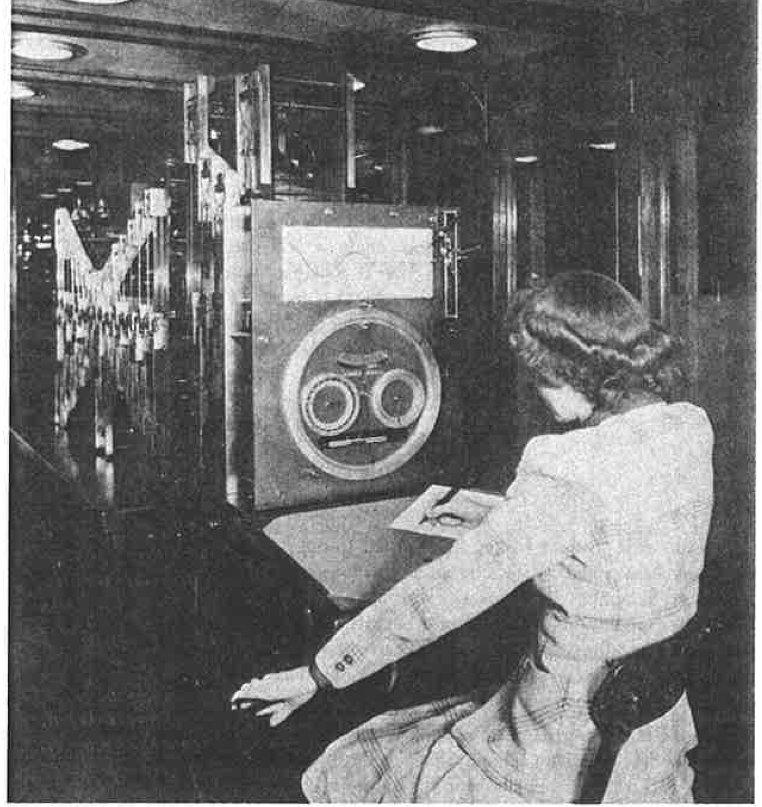
\includegraphics[width=\textwidth]{figures/images/zetler_tidal_computer_lady_1921.png}
	    \caption{Harris-Fischer tide machine circ. 1912 \protect{ \citep{Parker:2007wq} }}
    \end{subfigure}
    \hfill
    \begin{subfigure}[t]{\figwidthHalf}
    	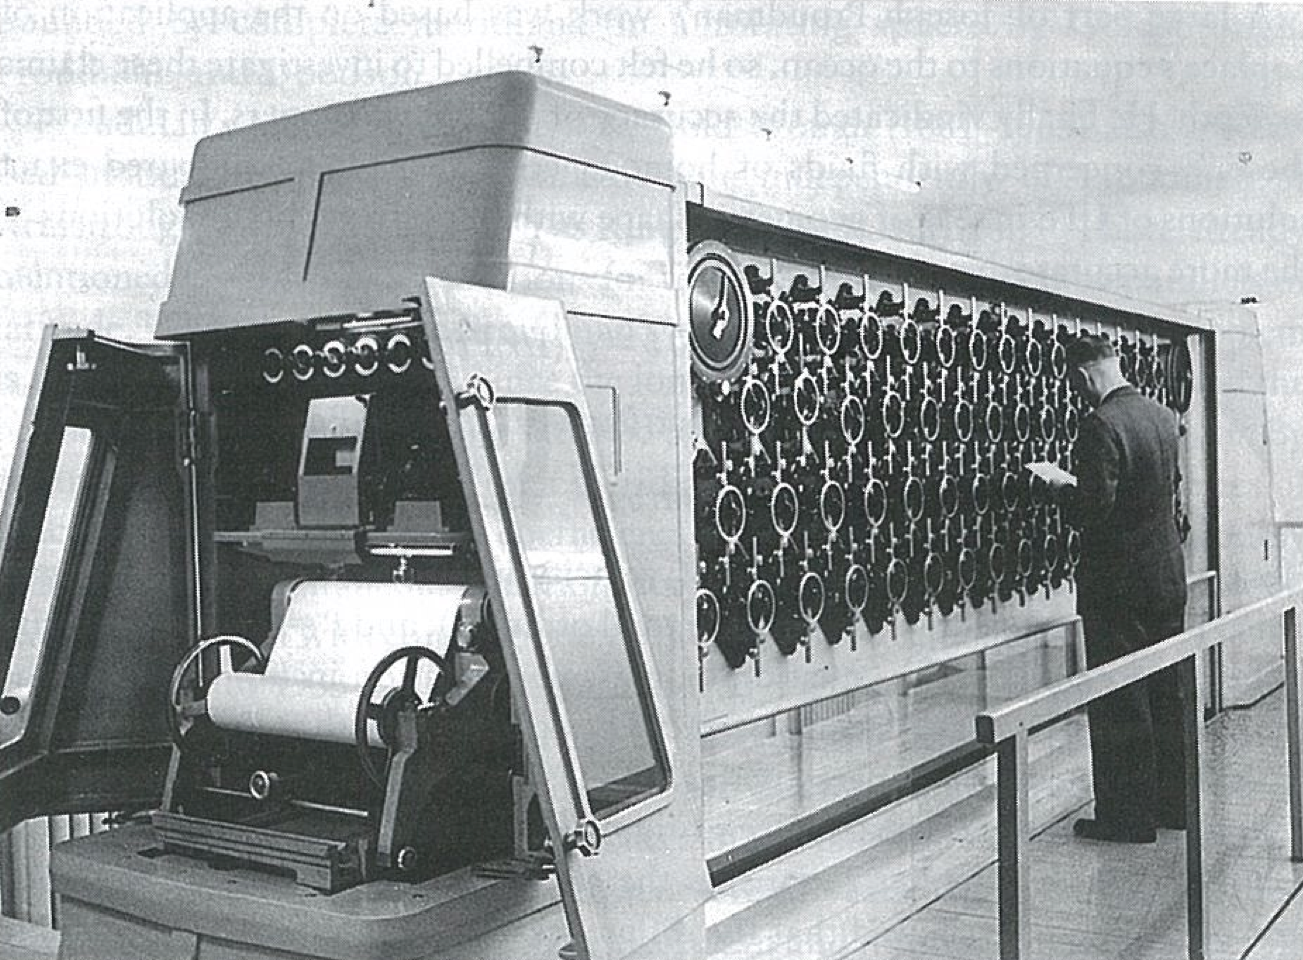
\includegraphics[width=\textwidth]{figures/images/DHI_machine_cartwright_fig11p2.png}
	    \caption{Gezeitenrechenmaschine at DHI circ. 1940 \protect{ \citep{Cartwright:2000tt} }}
	\end{subfigure}
	\caption{Analogue tide machines embody harmonic prediction.  A finite set of phase and amplitude values are dialled up and the handle turned to generate a prediction timeseries.}
	\label{fig:tide_machines}
\end{figure}
%----------------------
Harmonic analysis can be formulated as an over-determined inverse problem:
%--------------------
\begin{equation}
    \label{E:Axb}   
    \M{A} \V{x}=\V{b} 
\end{equation}
%--------------------
Where $\M{A}$ is a matrix of tidal timeseries basis functions, $\V{x}$ is the analysed tidal solution and $\V{b}$ is an observational record. The tidal basis functions are developed from the combination of the harmonic decomposition of $\eta_{eq}$ and a series of conventions.  The resulting basis is neither orthogonal nor complete. Inclusion of the modulation terms $f_k$ and $u_k$, discussed below, means that the basis functions are not actually sinusoids. The core assumption of stationarity for the finite series of basis functions is equivalent to an assumption that the basis has infinite span in time.   

Practical applications of the harmonic formalism has largely evolved prior to modern cheap computing, and many details can appear somewhat baroque in isolation.  The analogue instruments shown in Figure \ref{fig:tide_machines} serve to highlight this operational history.


The harmonic idealisation effectively operates on infinite basis functions whereas any observational record is of finite length.
Given the close clustering of tidal lines in frequency-space, equation \ref{E:Axb} is poorly conditioned for inversion.   This matrix condition is further degraded by the presence of non-tidal variations. 
Subsequently, practical harmonic analysis procedures must specify which frequencies to include in the basis set and then somehow account for the effects of unresolved frequencies.

At the time of writing the Bureau of Meteorology process does not systematically account for the inversion quality with regard to signal:noise ratios as suggested by \citet{Foreman:2009bg}.
This fact contributes to the potential for overfitting or projection of non-tidal signal onto standard tide predictions discussed in chapter \ref{chp:aggregate} and \ref{chp:tideFlavours}.


When additional constants can be inferred rather than taken directly from the inverse solution, using assumed relationships from either $\eta_{eq}$ or previous or nearby analysis.




Typically arguments regarding the relative magnitude of the harmonic components of $\eta_{eq}$ are used to prioritise candidate frequencies for inclusion with respect to the observational  record length. 
By convention, the effects of clusters of unresolved tidal frequencies are represented by modulation of the basis functions in relationships assumed to map from $\eta_{eq}$.  
In equation \ref{eq:cos} these modulation terms are included as $f_k$ and $u_k$.  These terms are misleadingly known by convention as `nodal corrections', due historically to the close spectral spacing associated with the the lunar nodal regression; differences in $\omega_k$ of about $\fract{1}{18.6}$ years.     These same terms are more informatively called `satellite modulations' by some authors in recognition that the modulation of a constituent term by a very closely spaced spectral cluster arises from terms other than $d_5$. 

Importantly, this nodal modification of basis functions means that the analysis results do not simply represent amplitudes and phases for regular sinusoids.  





To the extent that the non-astronomical phenomena are regular enough to be predictably periodic, inclusion within the LTI model can be to the benefit of a tide prediction.   On the other hand, effects that are not perfectly aligned to the \ATGF{} conflict with the fundamental LTI model and necessarily present an additional risk to forecast skill.


For instance with seasonal phenomena.   The harmonic decomposition of $c_{nm}(t)$ provides two relatively tiny signals at periods of 1 and 0.5 years - conventionally termed Sa and Ssa.  Despite the small amplitudes in $\eta_{eq}$ there are powerful seasonal variations in ocean observations that project onto the Sa and Ssa tidal components.   This is well recognised and `...whether the calculated values of Sa and Ssa are used or not, becomes almost a philosophical question, based on ones application' \citep[p122]{Parker:2007wq}.   Related terms that reflect seasonal modulation of semi-diurnal components can also included be included in standard harmonic analyses (eg H1 and H2 in Foreman schedule \citep{Foreman:1977ua})\\
Perhaps more significant methodologically, is the case of diurnal and semidiurnal sea level signals driven directly by \emph{meteorology} rather than the \ATGP{}.   The tidal frequencies denoted S1 and S2 are a prominent case in point.  For instance, Ray and Ponte \citep{Ray:2003ui} evaluate \NWP{} representations of \emph{barometric} tides at these frequencies with implications for oceanographic processes.  Treatment of S1 and S2 in tidal sea level predictions is a point of difference between the harmonic and response methods.  The later going so far as to invoke a distinct input function in the form of a `radiation potential'.    The response approach is now discussed in more detail. 


% APPENDIX?


% response methods
The \underline{response method}, and it's variations, form the primary alternative to the conventional techniques of harmonic analysis.   This consists of a generalised implementation of the LTI model, in which the ocean response to \emph{any} input sequence is characterised by a stationary admittance function.  The terminology was introduced by the influential publication \citet{Munk:1966ts}.
The authors claimed to be motivated by an application of Ockam's razor to the highly evolved historical baggage of harmonic methods.   

Some more on this topic is addressed in Appendix \ref{appendix:response}, but is not essential to the flow of this discussion.


%-----------------%
%\subsection{Tidal admittances in operations}

% LTI
It should be re-iterated that at high level, the harmonic and response models contain the same core concept.   Both model the ocean as an LTI system responding to some type of tidal forcing and both contain assumptions about the smoothness of ocean admittance.  Indeed Le Provost in \citep[chpt6]{Fu:2001ub} groups both the standard harmonic and convolution formalism as instances of the `response' formalism on this basis. \\
By definition these LTI methods are aiming to represent phenomena stationary in tidal frequency-space.  Treatment of non-stationary tidal phenomena forms a scientifically important extension, eg \citep{Colosi:2006va} and \citep{Ray:2011tj}, but presently plays a very secondary role with regard to conventional sea level forecasts.\\
A point of special interest to the explicit resolution of tides within \OGCM{}s is the relatively small but observable sea level surface signatures of nonstationary internal tides.




% harmonics == admitance
Consistent with this equivalence, it is common within the literature to refer to harmonic constants \emph{as} admittances.   A harmonic constant is seen as a sample from the admittance curve at an exact frequency. For instance Smith\cite{Smith:1997ut} provides the simple conversion to sample $Z(\omega_{nmk})$ and scale by the \ATGP{} amplitude $H_{nmk}$.
Furthermore, harmonic constants remain the lingua franca of ocean tide discussions. Regardless of the detail behind any particular method, results are almost universally transformed into conventional amplitude and phase values for intercomparisons.\\
In less specialised language however, harmonic analysis is quite distinct from a response method - especially with regard to whether the outcome is a list of constants or a series of admittance curves.\\




% inference and smooth
Regardless of the method used for analysis, an expectation that admittance curves $Z(\omega)$ should not contain discontinuities or sharp changes (the `credo of smoothness') is commonly evoked to enhance the spectral content upon the \emph{synthesis} of a tidal timeseries.  Following an analysis performed to determine admittances at a relatively small number of frequencies, $Z{\omega}$ is interpolated or extrapolated in frequency-space to infer additional spectral information.   The design of such an inference process can treat frequencies on a case-by-case basis distinguishing between component admittance curves (for instance \citep[pp 268]{Fu:2001ub}).




% operations
There is an apparently wide gap between the practices of centres producing \underline{tide tables} using conventional harmonic analysis and the more varied and advanced methods used within the scientific literature and employed for global models.


The relative significance of non-linear effects between the vast open ocean and the coastal zone provides some explanation for this split.  As illustrated in Figure \ref{fig:response}, the manner in which nonlinear feedbacks are incorporated into the response formalism significantly reduces it's elegance in comparison to the purely linear application valid for blue-water tidal analysis.\\
Another factor contributing to this gap is largely cultural.
\begin{quotation}
$\dots$ the improvement in predictable variance is numerically small compared with the natural noise in sea level.   Because of this, and the fact that the Response Method is harder for a routine operator to grasp, it has never been adopted for ordinary tide-table production. It remains essentially a research tool for specialists. \citep[pp 198]{Cartwright:2000tt} 
\end{quotation}
Expanding Cartwright's explanation, the importance of robustness and intuitive error checking to routine operations should also be emphasised.  Short tables of constants are indeed physically intuitive and facilitate simple checking.   And the presentation of spatial atlases for amplitude and phase are standard.





%-----------------%
\subsection{Distinguishing forecasts and filtering}

Sea level forecasting is not the only reason for employing tidal methods in operational centres.\\
Tidal methods are employed for two broadly distinct purposes: forecasting and filtering.  And beyond the operational context even more varied tidal methods are employed for data analysis and specialised studies.\\

The distinct motivations behind producing a forecast and filtering a signal can lead to significant differences in what is defined as the tidal component of observed sea level.   Subsequently, apparently inconsistent tidal timeseries can be in simultaneous use within an operational centre.



Filtering to remove tides from an ocean signal is commonly referred to as `de-tiding'.  Filtering is a means to distinguish signal and noise.  Application of a de-tiding process categorises tidal variations as noise so as to make use of the remnant signal.   In that respect de-tiding is nominally the inverse problem to tidal analysis.   Following the discussions in Section \ref{sec:semantics}, important details regarding what should be defined as tidal then naturally depend on the context of an application.\\
Operational oceanography in the form of \BL{} relies on de-tided altimetry observations as an important assimilation constraint.   The de-tiding process has been designed to render the observations compatible with the physics of the model, with a focus on meso-scale baroclinic variability. The current configuration of \BL{} does not assimilate tide gauge data, though in principle these insitu observations could be rendered consistent via appropriate de-tiding, for example \cite{Matsumoto:2000tg}.
%-------------------------
\begin{figure}[h]
\begin{center}
    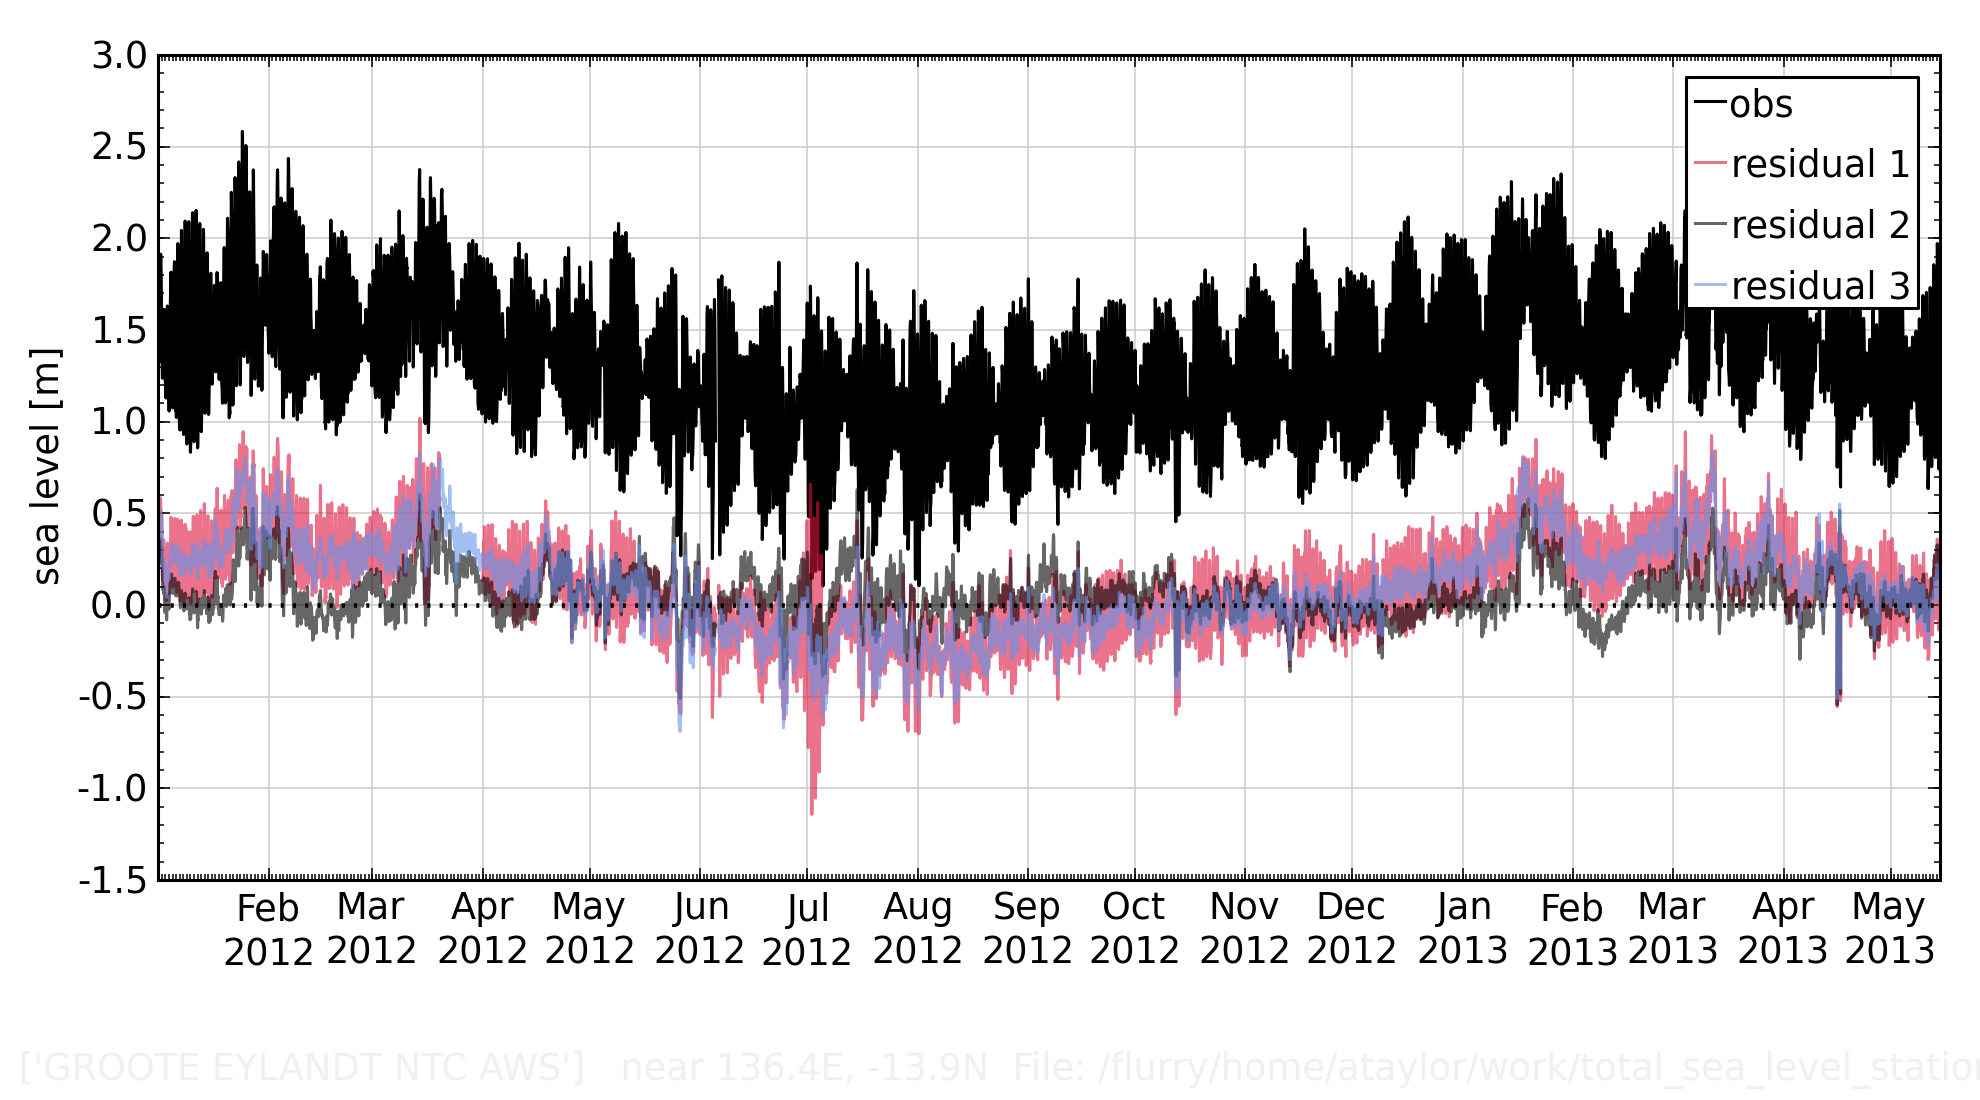
\includegraphics[width=\figwidthFull]{figures/plots/diag_plot_014406_detide_compare_20120101.png}
    \caption{Illustration of de-tiding observations by subtraction of tide predictions.  Different `residuals' result from alternative tide predictions: [1] regional gridded tide solution, [2] harmonic prediction and [3] harmonic prediction with significant non-gravitional harmonics removed. }
    \end{center}
\end{figure}
%-------------------------
Altimetry observations are de-tided via subtraction of a tidal signal synthesised from a global model.  There is no unique manner in which to specify the correction, with many options and `flavours' available from standard sources such as RADS \citep[table 3.2]{Scharroo:2011vd}.  The details of how the tidal correction is constructed can have implications for interpretation of the final ocean forecast.   The treatment of long-period tides \citep{Egbert:2003jd} and nongravitational tides \citep{Arbic:2005gv} are highlighted as special points of interest with regard to operational sea level forecasts.\\




In contrast to the situation with filtering, dynamical cause and effect are only relevant to stand-alone tidal forecast products insofar as they impact predictability.  From a users perspective, tide tables simply forecast sea level and ideally account for as much of the observed signal as possible.   By that measure it is proper that the tide tables include all of the reliably periodic signal regardless of cause.   
Thus the treatment of long-period harmonics Sa and Ssa is `philosophical question' \citep{Parker:2007wq} insofar as any reliably periodic signal at these relatively low frequencies can be determined from the observational record.  It is then not surprising that even amongst Australian tide authorities treatment of long-period signals differs enough to warrant special review attention \citep{MHL2156}.

% wavelets etc
For completeness it should be mentioned that other analysis techniques exist in the literature that are less directly relevant to the provision of sea level forecasts.


For instance, specifically tidal applications of wavelet analysis have been described as tools to provide insight into non-stationary tidal processes \citep{Flinchem:2000kp}.



%-----------------%
\subsection{Spatial tide models}
\label{sec:spatialTides}
Satellite altimetry motivated the extension of the empirical analysis methods discussed above to the production of regional and global atlases of ocean tides.  Indeed, tidal analysis formed an important driver and design constraint on the development of satellite altimetry missions.\\
Global tide models are commonly employed as intermediate products for other calculations well beyond the purposes of sea level forecasting per se.  For instance in the quantification of gravity effects, orbit determination, earth rotation and even the definition of coordinate systems \citep{Anonymous:2004tm}.\\



Meaningful tidal atlases existed prior to altimetry, most significantly that due to Schwiderski \citep{Schwiderski:1983ke}, but these necessarily suffered from a lack of validation and constraint in the deep ocean.\\
The basic premise of a tidal atlas is to present maps of tidal admittance at discrete frequencies, typically as separate amplitude and phase diagrams.   In line with the discussion in Section \ref{sec:LTI}, the deep ocean is conceived as a LTI system that is by definition stationary.  Each component wave can also be called a partial tide.\\
It is conventional to present atlas tidal predictions as separate maps of amplitude and phase for a single frequency.  These are also called `co-tidal' and `co-range' plots.  This visualisation fits well with the concept of the tidal ocean as a linear sum of standing waves.   The long spatial scale of these component waves and the existence of spatial nodes places special importance upon \emph{amphidromes} or \emph{amphidromic points} - nomenclature introduced by Harris in the late 19th century \cite[pp 119]{Cartwright:2000tt}.  Existence and placement of amphidromic points is an important visual metric employed to assess tidal model results \citep{foreman:2012perscomm}.  Figure \ref{fig:atlas} shows a the typical tidal atlas result with amphidromic systems apparent as radial patterns in the co-phase diagram.


Modern tidal atlases are in close agreement with regard to broad patterns, but characteristically differ at the shallow water margins; the very location of most direct interest to sea level forecasts.  Figure \ref{fig:tpx_cross} illustrates the fact that modern global tide models typically agree within about 0.02m in the deep ocean, but can differ substantially in coastal and shelf regions.  
%---------------------------
\begin{figure}[h]
    \begin{center}
    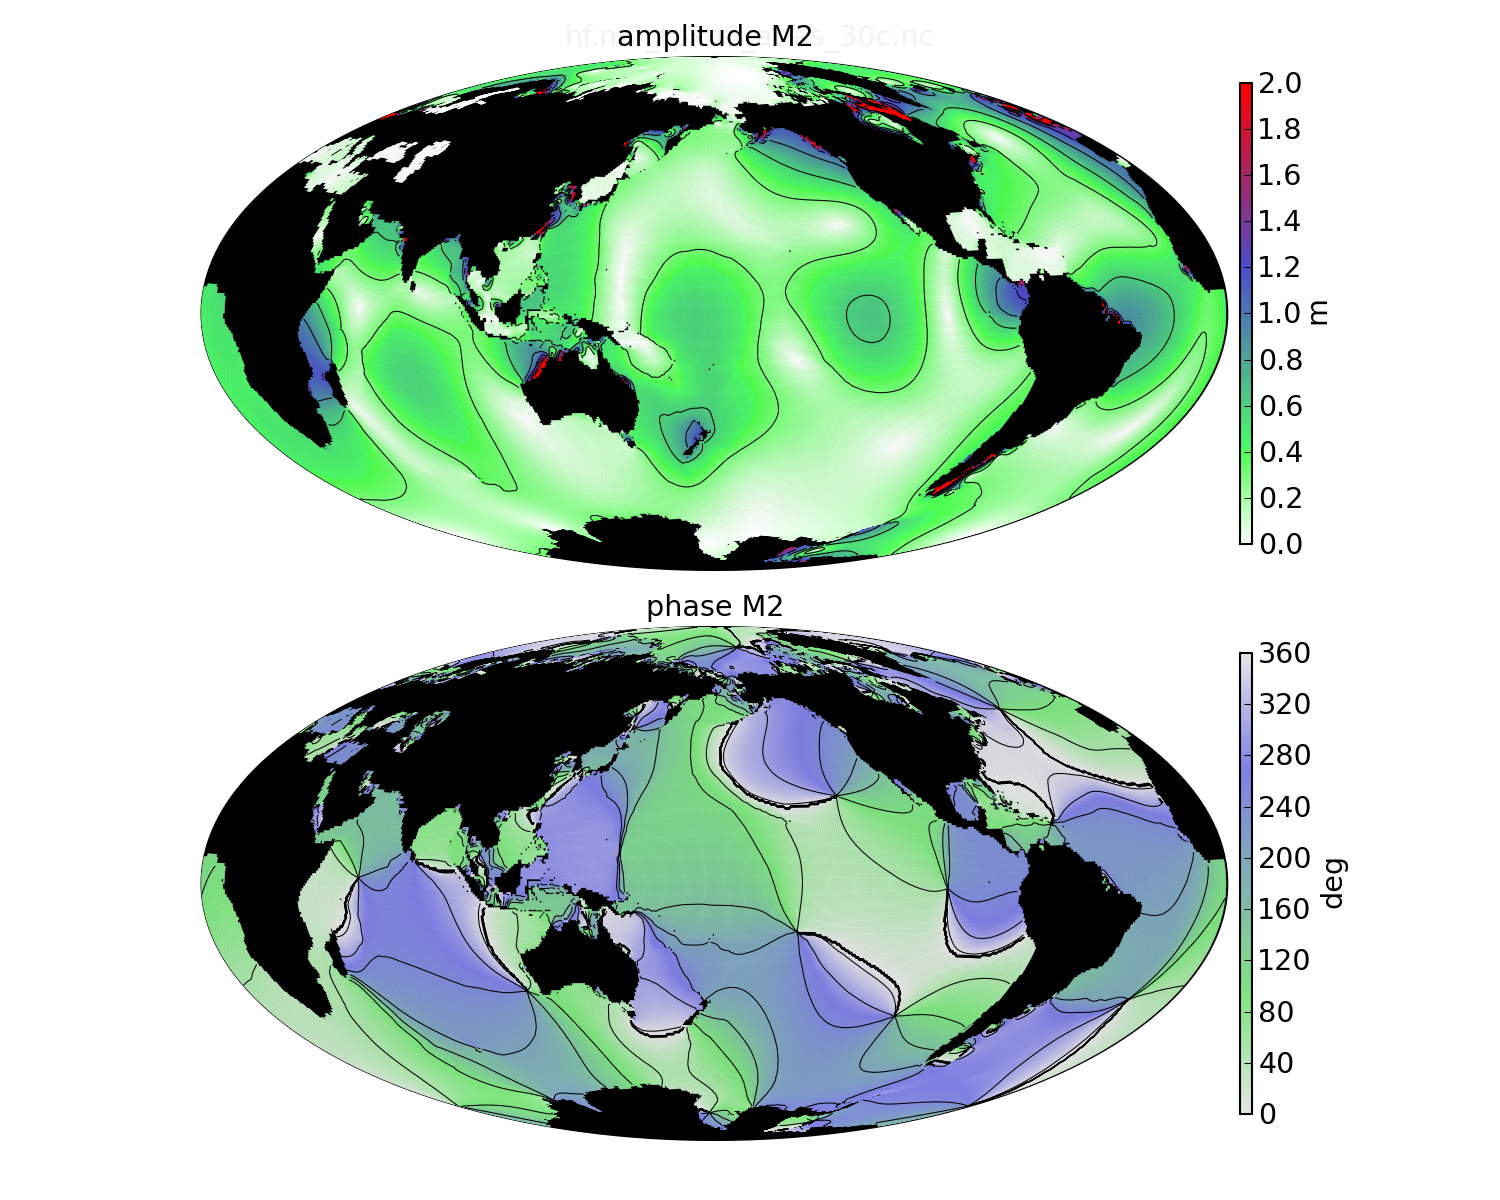
\includegraphics[width=\figwidthBig]{figures/maps/global_m2_tpx08.png}
    \caption{Example tidal altas showing cophase and corange diagrams for a single tidal component M2.  Data source TPX08 \cite{Egbert:2002ug}  }
    \label{fig:atlas}
    \end{center}
\end{figure}
%---------------------------
\begin{figure}[h]
    \begin{center}
    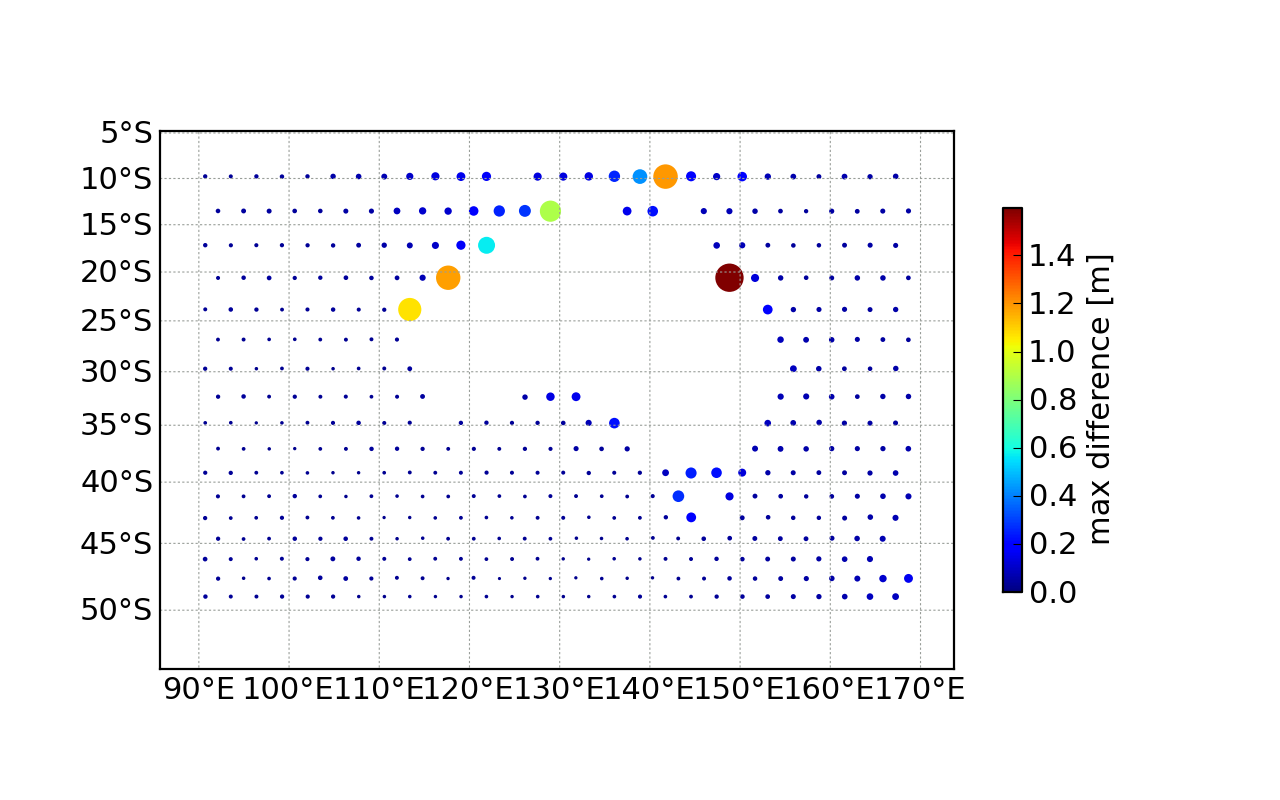
\includegraphics[width=\figwidthBig]{figures/maps/map_tide_differences_tpx_xovers.png}
    \caption{Maximum difference between tidal timeseries for 2012 at topex cross-overs near Australia.  The different solutions agree very closely in deep water, whilst the significance of shallow water effects are apparent.  Models included: CSR04\citep{Eanes:1996tr}, FES04\citep{Lyard:2006ir}, DTU10\citep{IMPROVEMENTOFGLOBA:2010tu}, GOT47, GOT48\citep{Schrama:1994vr}\citep{Ray:1999vm} }
     \label{fig:tpx_cross}
\end{center}
\end{figure}
%---------------------------

The LTI concept embodied in tidal atlases is well suited to representing deep water tides.   Amplitudes of each partial tide are no larger than about 0.02 cm for the majority of the global ocean, compared to depths of around 4km.
Given the underlying LTI framework, the tidal literature has naturally focused on stationary frequency-space metrics.  Intercomparison of mode1s and assessment against observations is almost always performed at a small set of dominant tidal frequencies - commonly only M2, K1, O1 and S2.


Tidal atlases are in essence no different from one-dimensional tide predictions.   Preceding discussions regarding the varied formalisms [Section \ref{sec:formalisms}] apply equally to regional atlases as to insitu timeseries.  Similarly to insitu tidal products, special attention is warranted regarding the treatment of signals associated with non-gravitational effects and the possible differences between a forecast model and an correction/filter.



Whilst some authors have presented the existence of repeat-orbit altimetry observations as effectively being `thousands of tide gauges', reduction of these observations via tidal analysis requires many special considerations.  For instance, infrequent but regular observation of any one surface coordinate places special importance on aliasing effects.



Despite the general equivalence, a point of practical difference is the treatment of the non-linear effects significant in shallow water.
In contrast to the apparent convergence of surface tide models in the open ocean, shelf and coastal regions are problematic.   In shallow waters wavelengths shorten and nonlinear interactions between partial tides can become very prominent.  \\
A strength of conventional 1-dimension analyses of coastal tide gauges has been the incorporation of shallow water compound tides.  It is not atypical in Australian locations to include dozens of nonlinear frequencies in a harmonic analyses.   Nonlinear signals observed at a tide gauge are often due to complex very localised dynamics, and the spatial projection beyond the observation point is non-trivial.  Understandably, global tidal atlases have generally focussed attention on the linear deep water signal and have poorly represented or ignored coastal nonlinearties.  The nonlinear M4 signal (associated with self-interaction of M2 waves) is perhaps the only such partial tide to be included in many modern atlases and is observable with altimetry \cite{Ray:2010jm}.


As a forecast product, tidal atlases have nothing like the broad economic integration of conventional coastal tide tables.  The Australian Bureau of Meteorology does not promulgate official tide predictions away from insitu observation locations. 
For the contemporary operation setting, tidal atlases are primarily relevant as an intermediate product to enable satellite observations.



Coordinated development of improved tidal atlases with specific performance requirements formed a significant component of altimetry missions in the 1990s.
\begin{quotation}
This international effort quickly split into two main approaches: the so-called empirical approach based on the direct analysis of the altimetry sea level time series \dots{}, and a modelling approach based on hydrodynamic and assimilation models. Later on, the interaction between the two approaches (i.e. data assimilation based on altimetry analysis on one hand, and hydrodynamic/assimilation modelling on the other hand) was a key factor for the overall success in improving tidal prediction accuracy and reaching the T/P requirements \cite[pp394]{Lefevre:2011dg}.
\end{quotation}


%%-----------------%
%\subsection{Global tide solutions and data assimilation}

TBC!! 


No global tidal atlas can be purely empirical - the spatial and temporal coverage of observations is too sparse.\\
Schwiderski's pre-altimetry solutions relied heavily on global compilations of harmonic constants for mainly coastal tide gauges, from which spatial maps were created via a `hydrodynamic interpolation' method that would in hindsight be considered an application of data assimilation \cite[pp822]{Egbert:1994wz}.\\
Now with around 20 years of altimetry data, all the highly evolved global tidal models or \emph{tidal solutions} in use all employ data assimilation in some manner.  That is, they make some combined use of dynamic models and observational data.  This includes a reliance on supporting geophysical models and corrections implied by the use of altimetry observations.\\



The dynamics relevant to tidal sea level are conventional written as the Laplace Tidal Equations (LTE) - for instance \cite[9.8]{gill1982atmosphere} and \cite{Hendershott:1981ub}.   
Via a series of assumptions, the LTE are a set of depth integrated shallow water equations in a rotating thin shell.  Advection is neglected altogether.\\
The LTE evolve a simple 3 dimensional ocean state consisting of horizontal mass transport and sea level perturbation. In time domain, the LTE can be written following the notation and discussion of \cite[pp185]{Egbert:2002ug}:
%----------------------
% LTE in time-domain
\begin{align}
    \label{E:LTE_momtm}
    \frac{\delta \mathbf{U} }{ \delta t} + f\vec{k} \times \mathbf{U} + gH\nabla \eta  + \mathbf{F} &= \mathbf{f_0} + gH \nabla \eta_{SAL} \\
    \label{E:LTE_cont}
    \frac{\delta \mathbf{\eta} }{\delta t} &= -\nabla.\mathbf{U} 
\end{align}
%----------------------
Where $\mathbf{U}$ is the depth integrated horizontal transport, $\eta$ is the sea level signal, $H \gg \eta$ is mean water column depth, $f=2\Omega\sin\theta$ is the Coriolis parameter and $g$ vertical gravitation.\\
The forcing terms on the right hand side of the momentum equation \label{E:LTE_momtm} require explanation.  
$\mathbf{f_0}$ denotes the astronomical body forcing taking into account earth tide effects, $\mathbf{f_0} = gH\nabla\eta_{eq}$ following Equation \ref{eq:VT}.  
An approximation for SAL is here written as a separate forcing term to reflect the suitability of using values pre-computed from existing global tide models.   
Alternatively $\eta_{SAL}$ can be put on the left hand side of the equation as a scaled version of $\eta$ - as is the case in \MOM{}.   
This scalar approximation is relatively inaccurate as discussed in section \ref{sec:basic_potential}.\\
The frictional dissipation term $F$ is a particular source of complexity, especially with regard to parameterisation and linearisation.\\

Compared to the dynamics represented within an \OGCM{}, these tidal hydrodynamics simulate a more `aggregated' psuedofluid in that the processes contained within parameterisations are have a higher degree of complexity - as per the schematic in Figure \ref{fig:models} \\
\begin{quotation}
Forward global tide models are an ideal testing ground for the hydrodynamical cores of numerical ocean general circulation models, and for ideas about drag and dissipation. In contrast to data-constrained models, forward models cannot achieve accurate tidal elevations unless substantial parameterised drag is included in the abyss. Forward models thus point clearly to drag in the open ocean as a central control on tidal flow.\citep{Arbic:2004wz}
\end{quotation} 


Linearisation is important in the tidal context to facilitate transformation of the LTE into the frequency domain.   Given the tidal LTI framework, the ultimate solution of a tidal model is the evaluation of static admittances or constants.   One approach towards this end would be to integrate the LTE in the time-domain and subsequently reduce the output to a series of harmonic constants via conventional analysis.   The celerity of barotropic waves in the deep ocean is relatively fast and thus requires short time-steps.   Assuming linearity and the existence of a convergent solution in frequency-space, the LTE can be solved directly in spectral form with greater computational efficiency.   The efficiencies are especially important upon the application of data-assimilation methods that involve both a backward and forward iteration of the dynamics \cite[pp184]{Egbert:2002ug}.


Again following the notation of \cite[pp186]{Egbert:2002ug}, the LTE at a single tidal frequency $\omega$ can be written:
%----------------------
% LTE in freq-domain
\begin{align}
\label{E:LTE_momtm_w}
\mathbf{\Omega} \mathbf{U} + gH\nabla \eta &= f_u \\
\label{E:LTE_cont_w}
\nabla.\mathbf{U} + i\omega\eta &= f_\eta\\
\mbox{where   } \Omega             &=
\left[ \begin{array}{cc} 
      i\omega + \kappa & f \\ 
       -f              & i\omega + \kappa  
                        \end{array} \right]   \nonumber
\end{align}
%----------------------
Where $\kappa$ is a linearised approximation for the dissipative stress.   Frequency-space forcing terms $f_u, f_\eta$ are written in both equations for generality with regard to data assimilation (inversion).  This frequency-space approach is common to other data assimilative tidal models such as FES \cite[pp395]{Lyard:2006ir}.\\
Nonlinear terms can be incorporated but complicate the formulation of any inversion.


Whilst numerically solving the LTE is quite tractable and comparatively simple, significant uncertainties prevent a direct `free' or `forward' model from producing accurate forecasts.  Hence the importance of data assimilation or generalised inversion methods.  Solving the LTE is complicated by spare observations and ``$\dots$ the need for accurate open boundary conditions and bottom topography, the need for approximate parameterisations of dissipation in the tidal equations, solid earth effects, and the effects of ocean stratification on the barotropic tides, which may be difficult to account for without full 3D modelling of baroclinic tidal currents''\citep[183]{Egbert:2002ug}.

A comparative description of data assimilation methods in the context of tide models is laid out by Egbert and Bennet \cite{Egbert:1996vr}.



Summaries that categorise the many global tide models on the basis of design choices, parameterisations and data assimilation methods are given in \cite{Ardalan:2008gs} and \cite{Matsumoto:2000tg}. \\

%   ??  Application of the LTE is not restricted to the barotropic surface tide.   The formulation can be extended to represent stationary internal tidal modes via use of equivalent-depths .\\
% Energy cascades.??\\

The barotropic hydrodynamics used in global tide models has proven to be an appropriate level of aggregation when the aim is to map tidal patterns of surface elevation.  The LTE provide a tractable means of doing so given the incomplete spatial and temporal coverage of observations.

But consideration of tidal dynamics naturally raises the topic of \emph{internal tides} and the separability of stationary barotropic tides from other ocean dynamics.
\begin{quotation}
Barotropic tides generate internal tides, and internal tides in turn feed back onto the barotropic tides. Inferences from altimetry-constrained barotropic tide models show that about one-third of global tidal energy dissipation occurs in regions of rough topography, where internal tides are generated \dots{}. Internal tide generation thus acts as a damping mechanism for the barotropic tides.\citep[pp22]{Arbic:hy}
\end{quotation}
Depth integrated barotropic LTE relegate the effect of internal mechanisms on surface elevation to parameterisations.  Dissipative stress $F$ in \label{E:LTE_momtm} stands for all losses of energy from the barotropic pseudofluid.  Given the reality of ocean stratification, these losses notably include conversion form the barotropic to higher baroclinic modes \cite[pp121] {gill1982atmosphere}.


For the present topic of sea level forecasting, internal modes are ostensibly of interest insofar as they impact the prediction of surface elevation.  Internal waves at tidal frequencies do have an observable surface signature albeit relatively small \cite{Ray:2011tj}.

More importantly for forecasting is the effect of the internal ocean state on the prediction of barotropic surface elevation.  A-periodic variation of the internal density structure of the ocean is of particular relevance as   conventional tidal analysis relies upon periodicity for predictability.     The tidal view of the ocean as a LTI system driven by the \ATGP{} is very useful, but with the caveat that ``the ocean is a physically complex and noisy filter.  In consequence, tidal harmonics are not strictly constant \citep[197]{Ray:2010jm}''.


Whilst stratification and internal mechanisms are very coarsely parameterised in dedicated tidal models, the internal structure of the ocean is a primary focus of \OGCM{}s.   The following section addresses the intersection of \OGCM{}s and tidal forcing with regard to sea level forecasts.


%-----------------%
\subsection{No singular ocean tide requirement in operations}

TBC .... 
whereas tidal manuals exist such as \citep{PCTMSL-sp9}, \citep{IOC:2005tj}, \citep{Level:2011wu}and \citep{Parker:2007wq} the operational details of practices are not generally published. 



A range of auxillary and derived from conventional tidal methods
- reference planes like HAT
- 



This lack of clarity motivates proposal in Chapter \ref{chp:tideFlavours}



detiding filter for non-tidal models taken up in the next section ....
\section{Mesoscale operational oceanography}
\label{sec:mesoscaleOperational}
Tide prediction has effectively been part of routine operations for several decades; whether or not the term ``operational'' has been applied.
Starting in the early 2000s, mesoscale ocean prediction has become operational in a manner that lagged and imitated the path of \NWP \citep{Harper:kb} rather than tide prediction. 
Like modern weather forecasting, operational oceanography is similarly a big science enterprise \citep{Petersen:2012tr} in the sense that it fundamentally relies on the coordination of large organisations, global networks and capital. 
The size and nature of this type of prediction stands in stark contrast to the ``small'' well-established practices of conventional tide prediction introduced in section \ref{sec:tidesOverview}.
The international Global Ocean Data Assimilation Experiment \GODAE{} serves as a historical reference point for how mesoscale prediction came into operational agencies like the Bureau:
``\textit{the central idea of \GODAE{} - to demonstrate the feasibility and utility of real-time, global ocean forecasting - was based on the experiences of the meteorological community in \dots{} FGGE}'' \citep{Bell:2009uv}.
From this original feasibility demonstration, the enterprise of mesoscale ocean forecasting has continued to mature across many national weather agencies; and the Australian case is documented by \citep{10.1080/1755876x.2019.1685834} in reviewing over 15 years of operational services.


In contrast to conventional tide prediction, sea level of itself is not the target of mesoscale forecasting; let alone coastal sea level.   But sea surface elevation is an important state variable for which forecasts are produced.  What these forecasts actually represent is not self-evident.  The manner in which sea level and tides are handled in systems like \BL{} is worthy of exposition in order to underpin the subsequent chapters describing methods for combining and evaluating sea level derived from these operational forecasts. 
  
%-----------------%
\subsection{Ocean general circulation models}
Ocean General Circulation Models (\OGCM{}s) are now a key component in oceanographic forecasting, but are only rendered operationally useful by the use of a global observation network and data assimilation to routinely maintain alignment with reality.
How this representation of reality relates to coastal sea level is however not self-evident.



An \OGCM{} simulates the physical ocean state via time step integrating a mixed boundary-condition/initial-condition problem.
In contrast to the tidal LTI conception of the ocean described in section \ref{sec:LTI}, an \OGCM{} conceives the global ocean as a turbulent continuum fluid; and the time and length scales of this turbulence effectively have no lower bound. The simulation thus needs to represent information cascades between turbulent scales as well as account for unresolved processes with sub-grid scale (SGS) parameterisations.
The distinction between resolved and unresolved scales is paramount.  ``Sensitive dependence on initial conditions in this turbulent flow \dots{} severely limits predictive capabilities [and] motivates a formulation of averaged or mean field fluid equations'' \citep[Sec 2.5]{Griffies:2004vs}.
Furthermore, this raises broad questions of how to interpret the output of a numerical ocean simulation.
Griffies perceives an \OGCM{} as representing the averaged motion of an infinite ensemble of hypothetical oceans; the imagined spread being proportional to the scales of SGS parameterisation.
Alternatively, \citet{Stevens:2001kb} casts \OGCM{}s into the class of geophysical ``pseudofluid'' simulations. Of which he notes comparisons with observational data are prone to interpretational nuance and are ``too often ad hoc, uncritical, and/or irrelevant''\citep[pp 286]{Stevens:2001kb}. 
Figure \ref{fig:ogcmScales} illustrates very schematically the place of \OGCM{} variants in the context of turbulence simulations.   The exclusion or explicit representation of tidal dynamics are shown as changes in SGS complexity; these are discussed further below.
%----------------------------------
\begin{figure}[h]\centering
  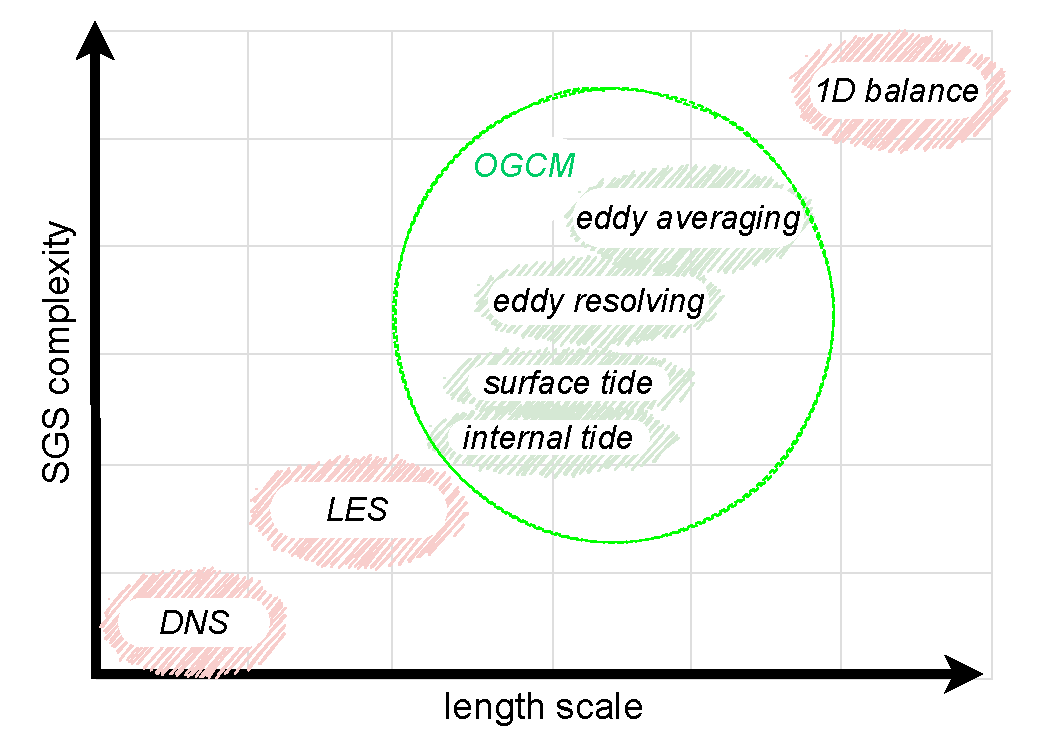
\includegraphics[width=\figwidthBig]{figures/diagrams/ogcm_scales.pdf}
  \caption{Schematic place of \OGCM{}s in terms of sub-grid-scale parameterisations.}
  {Schematic illustration of place of \OGCM{}s in terms of the sub-grid-scale (SGS) parameterisation of the broad scale range of a turbulent ocean.  For reference, methods from turbulence studies are included: Direct Numerical Simulation and Large Eddy Simulation. Following \citep[fig 5.2]{Petersen:2012tr} and \citep{Stevens:2001kb}.  Explicit tides in an OGCM represent a reduction of parameterisation without a large change in spatial scale resolution.}
  \label{fig:ogcmScales}
\end{figure}
%----------------------------------
Common to big science simulation practice more generally \citep{Petersen:2012tr} any real \OGCM{}, including \BL{}, embodies a significant accumulation of human effort in the very many lines of computer code.  In contrast to typical tidal analysis tools, the software behind a mesoscale ocean forecast is effectively too much for any one person to understand in detail.
%-----------------%
\subsection{Data assimilation and sea level observation}
Data assimilation is the model-data-fusion framework by which the initial conditions for each \OGCM{} forecast are determined.
This processing step can be usefully viewed from a Bayesian perspective in which ``the system implements an optimality criterion which defines how to best combine dynamics and observations, given an hypothesized error model for both.'' \citep{10.1007/978-94-007-0332-2_13}.
Subsequently the availability of near-real-time observations of the global ocean has played a critical role in enabling operational mesoscale forecasting.  Expansion of ocean observation coverage of recent decades largely mirrors the maturation of abundant satellite communications.  But despite the growth of what has been called the global ocean observation system \GOOS{} \citep{Komen:1999ch}, the ocean remains fundamentally under-observed for the purposes of physical state estimation.   Satellite-based surface observations of the ocean are the most abundant, whilst the ocean depths are sampled by comparatively sparse insitu profiles.


Tide gauges observations are fundamental to conventional tide prediction, but are in contrast often totally excluded from mesoscale data assimilation.   The fact that \BL{} does not assimilate any sea level data from tide gauges is relevant to the aggregated forecast design described in chapter\ref{chp:aggregate}.      
Sea level close to coast lines in a mesoscale ocean simulation is primarily an expression of the simulated fluid dynamics rather than an observationally constrained parameter.

Whilst tide gauges are excluded from assimilation, sea level observations derived from satellite mounted radar instruments are a crucial input and have played a pivotal role in the evolution of ocean forecasting in general \citep{Fu:2001ub}.  Moreover, the forecast skill associated with the assimilation of satellite altimeter data has been shown to be of particular significance by  \citep{10.5194/os-13-1077-2017} and others.
In contrast to the still water level observed by a tide gauge, it is primarily a sea level anomaly (SLA) quantity that is derived from the altimeters and used to constrain the \OGCM{}. Figure \ref{altimeterEg} illustrates the nature of the along-track nadir coverage of a single satellite altimeter.
These SLA observations are not however applied to constrain the ocean state in the vicinity of coastal tide gauges; and in the case of \BL{} are excluded from the assimilation process for regions where the depth is less than 200m or close to a land mass.   This reflects that fact that the derivation of sea level quantities from satellite altimeters is particularly challenging in shallow water and near coastal boundaries \citep{Woodworth:2011bf}.    Although an active area of development, coastal altimetry data streams are not yet used to constrain operational mesoscale forecast  systems.
%----------------------------------
\begin{figure}[h]\centering
  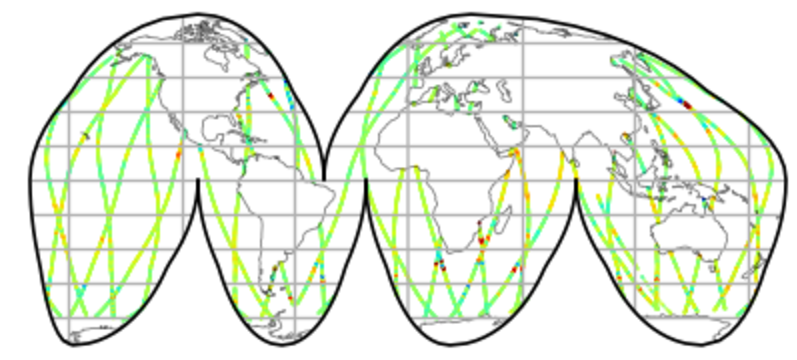
\includegraphics[width=\figwidthHalf]{figures/maps/altimeterCoverageEg.png}
  \caption{Spatial coverage of one satellite altimeter.}
          {Illustration of the typical spatial coverage pattern of a satellite altimeter. The along-ground track accumulated over a single day by Saral in May 2020 is shown. Observations near the coast are excluded from assimilation.}
  \label{fig:altimeterEg}
\end{figure}
%----------------------------------
SLA is a meaningful quantity to the extent that it is an anomaly from some reference, and that reference involves a spatial tide prediction; as introduced above in section \ref{sec:spatialTides}.
The role of tides in mesoscale forecasts is taken up in the following sections.
%--------------------------------------------------
\subsection{Treatment of tides in nominally non-tidal \OGCM{}s}
\label{sec:tides_ogcm}
Operational \OGCM{}s in the \GODAE{} genealogy have intentionally focused on non-tidal ocean dynamics. This focus has been motivated by the separation of time and length scales that allows for the simulation of relatively slow turbulent features at the mesoscale as a computationally tractable problem that can be adequately constrained by along-track altimeter observations.
In this view, much tidal variability is just the fast propagation of long wave length noise; a background sloshing of the barotropic ocean state not obviously connected to the evolution of eddies and boundary currents.
Moreover, the skill of spatial harmonic tide models in representing surface tides over the deep ocean facilitates the use of de-tided or filtered altimeter observations to constrain a mesoscale non-tidal simulation. In effect, the fluid simulation is split across two qualitatively distinct modelling approaches; an LTI frequency-space tidal ocean and a time-stepped turbulent mesoscale.  
\BL{} is a ``non-tidal'' system in that \ATGP{} forcing is not applied, and in contrast to local downscaled simulations, there are no lateral open boundary conditions. Not only does the mesoscale simulation exclude the gravitational tidal body forcing, it also excludes the surface boundary application of atmospheric pressure.   
Surface pressure is excluded as a forcing term for analogous time and length scale reasons as the tides.  In fact, for the barotropic mode the pressure and tidal forcing can be formulated in an identical manner as adjustments to the spatial gradient of the surface elevation as in \citet[equation 9.9.5]{gill1982atmosphere}.

The state variable quantifying surface elevation carried by the model is thus a peculiar sea level anomaly (SLA) which in itself is a rather abstract quantity. 
Using the \citet{Stevens:2001kb} nomenclature, \BL{} simulates an aggregated pseudofluid system with a qualified relationship to the actual ocean.


From that background, recent publications indicate a motivation towards more dynamic representation of the effects of ocean tides.   This is indicative of pervasive goal across numerical simulation practice to increase model concreteness by reducing the role of parameterisations \citep[section 5.3]{Petersen:2012tr}; a reduction of system aggregation \citep{Stevens:2001kb}.\\
Similarly, Griffies describes the ``general trend in ocean climate modelling towards reducing many of the common approximations'' \citep[pp20] {Griffies:2004vs}.   It could be said that the modelling community perceives parameterisations as a compromise that should ideally be replaced with explicit physics when computing power allows.

% split 
The timescales targeted by a mesoscale simulation are slow relative to surface tides.
Given the focus on estimating the slower baroclinic evolution on the three dimensional ocean state, operational ocean models following \GODAE{} take numerical approaches that employ some special treatment for the faster barotropic hydrodynamics. 
%rigid ild
Earlier models avoided direct representation of surface height variations by making the so-called `rigid-lid' approximation \citep[pp128]{gill1982atmosphere} which leads to other ramifications for ocean forecasting discussed by \citep[pp19]{Griffies:2004vs}.
% split explicit
The ocean model underlying \BL{}, \MOM{} \citep{Griffies:2008vh}, does carry a free surface height as a state variable by employing a `split-explicit' timestepping scheme.    
In essence, this approach timesteps a computationally cheap shallow-water representation of barotropic dynamics many times for each relatively expensive update of the full depth-dependant ocean state.  
Thus, by representing the barotropic free surface dynamics of the ocean, a mesoscale \OGCM{} like \BL{} could in principle simulate the global tides.
But tidal forcing is not applied in \BL{} and there are several high level arguments against doing so.
   
%-----------------%
\subsection{Motivation to explicitly simulate tidal effects}

Excluding tides from a mesoscale ocean simulation is essentially an undesirable but necessary design choice found to facilitate operational forecasting.
Barotropic tides interact with the baroclinic structure of the ocean, which in turn modulates the behaviour of barotropic waves; but the question as to if and to what extent these interactions can be paramaterised or ignored must be answered within practical constraints.
But design constraints are re-evaluated periodically; especially in light of the ongoing improvements in computational capacity and observation coverage.
Computational costs have reduced dramatically over the last decade and there is a motivation  to more explicitly simulate the role of tides in \OGCM{}s.
This motivation is primarily directed at representing the influence of barotropic tidal motions on the baroclinic mesoscale structure of the ocean state; not at directly improving the representation of total sea level.

Overall the tendency of geophysical simulation is towards every higher fidelity and concreteness - as discussed above. But the particular targets for a which some explicit simulation of tides in \OGCM{}s are aimed include:
\begin{itemize}
    \item improved spatial distribution of vertical mixing;
    \item improved simulation of barotropic/baroclinic energy conversion;
    \item improved resolution of frontal features;
\end{itemize}
These aims do not necessarily motivate an accurate simulation of the sea surface elevation.
Rather, in the spirit of Figure \ref{fig:ogcmScales}, it is a configuration with regard to what processes are relegated to sub-gridscale parameterisations.

Thus in the \OFAM{} simulations of \citep{Schiller:2004fv},  it was reasonable to include only a small subset of tidal constituents and make tailered adjustments to better match the astronomical phase information.  In contrast to a standard tide prediction,  the aim in this case was ultimately to improve the broad spatial distribution in which tidal currents influence mixing and water mass formation.

\citep{Arbic:2004wz} has highlighted the `inordinately large' magnitudes allocated to drag parameterisations in tide simulations generally, and the fact that large scale tidal simulations have to somehow account for the important role of barotropic to baroclinic energy conversion.   This conversion must be fully parameterised for a depth integrated simulation, but for a tidal \OGCM{} with baroclinic dynamics the line between what is explicitly modelled and what is parameterised is redefined.  

Inclusion of tidal motions within the HYCOM \OGCM{} has advanced substantially and been shown to benefit the representation of certain baroclinic ocean structures  \citep{10.1016/j.ocemod.2019.02.008}.    But this trajectory towards higher fidelity still relies on careful and tidally-specific parameterisation methods to account for unresolved processes; such as by the depth-dependant M2 ``wave drag'' term \citep{Jayne:2001tr}.

Some further comments on the explicit resolution of tides in \OGCM{}s is included in Appendix \ref{appendix:globalTides}



To date, the inclusion of explicit tides in \BL{} remains far from the Australian operational schedule.
But given the trajectory of operational forecasting more widely, the question of how to handle the boundary between tidal and non-tidal simulations will require continual revision.
One operational reference point for handling questions about differing representation of tides across numerical systems is provided from outside the \OGCM{} context; with the design of the United Kingdom Storm Tide Warning Service \footnote{now titled UK Coastal Monitoring and Forecasting}\citep{Horsburgh:2008gw}.   In this design the weather forecast simulation includes tides in order to account for non-linear interactions between the tidal and nontidal sea level effects; however this total water forecast is not applied directly, but is differenced with a tide-only simulation to derive a forecast surge (or residual) signal.   This configuration allows for both the simulation of interaction effects but the continued use of an established or superior representation of the tidal component.


Arguably the challenge presented by higher fidelity operational ocean forecasts is in how to usefully exploit these inherently incomplete and approximate representations;  
\textit{while a model can never be “truth,” a model might be ranked from very useful, to useful, to somewhat useful to, finally, essentially useless} \citep{Burnham:2002}.
The ability to rank usefulness and design forecast products will always be a function of the application, regardless of progress towards ever more concrete simulations.

%-----------------%
\subsection{Representation of coastal boundaries}
The numerical representation of the land/sea boundary is of special interest for the present focus on coastal sea level.
Model design choices that allow for the tractable representation of mesoscale ocean circulation properties stand in contrast to those that would specifically target coastal processes.
The image in Figure \ref{fig:oceanmapsMaskDetail} illustrates how the \BL{} spatial grid discretizes the Australian coast into approximately 10km steps.  A more national view is shown later in Figure \ref{fig:map_masks}.
At face value this resolution may appear too coarse to usefully simulate the water level at a coastal location; let alone within an shallow embayment such as Port Phillip Bay shown in the image.    But the length scales that can be represented rather lead to an expectation that the useful timescales of the simulation will be limited in some related way.   Chapter \ref{chp:aggregate} demonstrates that there is qualified value at the scales represented.
%---------------------------
\begin{figure}[H]
    \begin{center}
    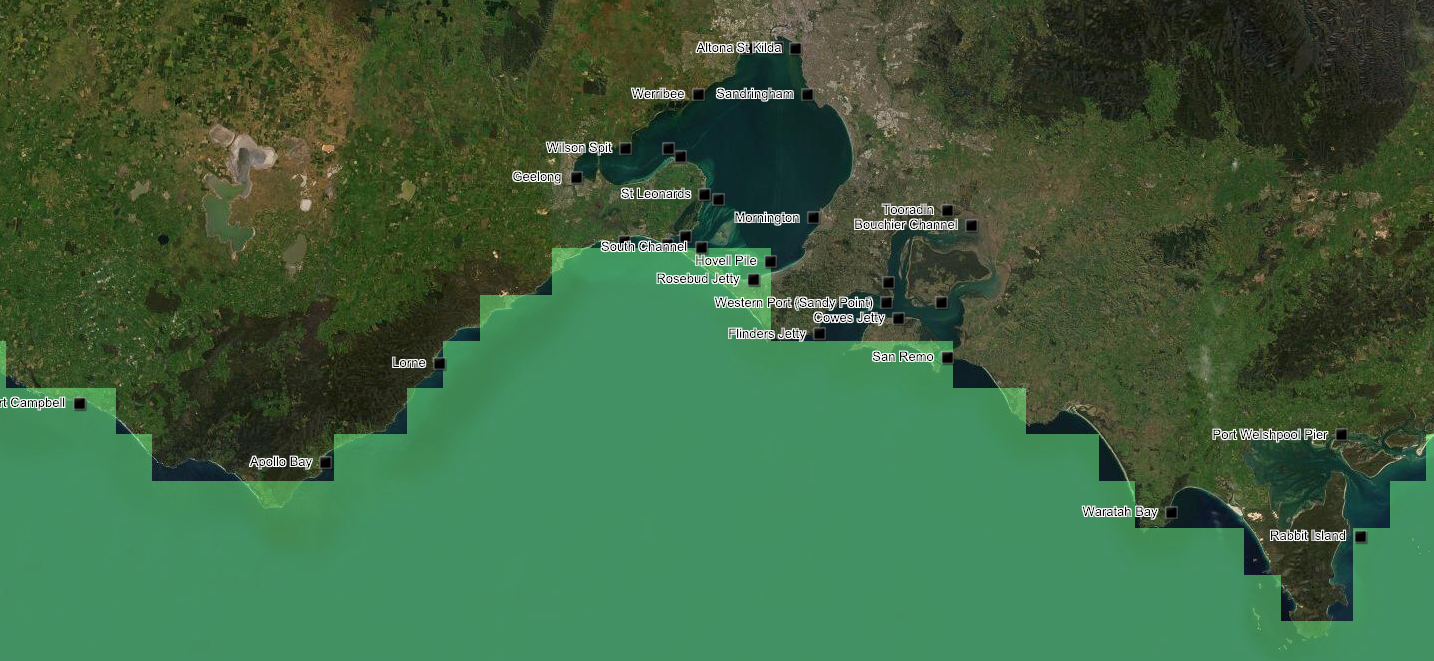
\includegraphics[width=\figwidthBig]{figures/images/oceanmapsMaskVic.png}
    \caption{Horizontal land/sea mask detail.}
            {Horizontal land/sea mask detail over south eastern Australia near Melbourne. The $0.1^{\circ}$ regular grid approximates the coast in ~10km steps and totally excludes features like Port Phillip Bay.}
    \end{center}
    \label{fig:oceanmapsMaskDetail}
\end{figure}
%---------------------------
But for the present document there are details beyond a nominal length scale that are worthy of explication.

Firstly, \BL{} simulates the ocean state on a regular Arakawa-B staggered horizontal grid.
This grid carries a fixed allocation of the land/sea mask, so there is no time evolution of where the coast is located as there could be in a system with the feature commonly called wetting-drying.
Furthermore, the system uses a fixed bathymetry and takes no account of sediment transport or any other active change to the lower boundary.

The staggered B-grid complicates how the coastal boundary is represented as there are effectively two horizontal grids that each determine what is wet and what is dry.
In particular, the sea level anomaly quantity ($\eta_t$) is quantified on the `T' or tracer cell grid.    However, in order to integrate the shallow water equations forward in time information is exchanged with velocity values carried on the `U' grid; and furthermore each timestep involves a spatial operation over a stencil of neighbouring cell points. 
The numerical implementation in \BL{} of the barotropic hydrodynamics leads the existence of a so-call checkerboard null-mode; a numerical artefact that can allow aphysical spatial discontinuities in sea level to grow.   To mitigate this null-mode, a spatial smoothing step is included within the fast barotropic integration.
%---------------------------
\begin{figure}[H]
    \begin{center}
    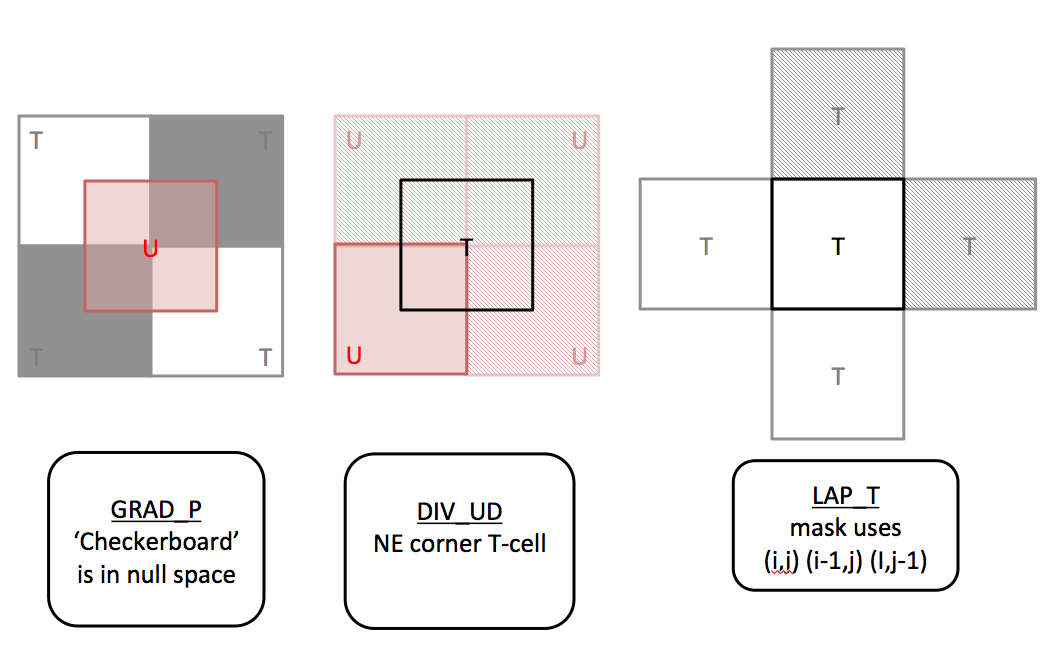
\includegraphics[width=\figwidthBig]{figures/diagrams/mom_BT_stencils_extra.png}
    \caption{Arakawa-B horizontal grid stencil illustrations.}
            {Arakawa-B horizontal grid stencil illustrations relevant to the baroptropic mode of \BL{}; the forecast sea level anomaly includes both barotropic and baroclinic contributions}
    \end{center}
    \label{fig:atlas}
\end{figure}
%---------------------------
These spatial considerations simply suggest that \BL{} should be able to simulate phenomena operating at length scales of several tens of kilometers.
But there are hydrodynamic processes that are inherently coastal, for which the relevant length scales are likely not isotropic and are more naturally cast in coordinates related to the coast itself.    
This topic is taken up in Chapter \ref{chp:waveguide} with regard to the representation of coastally trapped phenomena.





\section{Exploiting existing predictability}
\label{sec:exploitingPredictability}
%--------------------
\subsection{Unresolved processes and overlap}
All sea level forecasting systems are realised via design choices regarding what processes are in scope and the manner in which they are represented.
In the above sections, two operational approaches were contrasted; tide prediction and scale-limited hydrodynamic ocean circulation simulation.
To a first approximation these forecast types are conceptually complimentary; one being tidal and the other non-tidal, one in which the ocean is characterised by a time-invariant admittance and other by the evolution of a turbulent fluid. 
Each approach necessarily must account for the impact of unresolved processes on the target representation.


There are reasons to look critically at the nominal separation of these tidal and non-tidal forecast approaches.
Most simply, the fact that more than one conceptualisation of what comprises tidal sea level is in use operationally requires, at a minimum, semantic care to avoid misunderstanding.
More fundamentally, the boundary between resolved and unresolved will be redefined as simulation systems are updated and improved.  Hydrodynamic simulation in particular is set to continue in a direction of ever-higher fidelity and concreteness.

The motivation to explicitly represent tides in \OGCM{}s provides a clear case where the separation between tidal and nontidal would require revision.   
But some representation overlap of this nature is already present and is taken up in chapter \ref{chp:tideFlavours}.


Increasing simulation fidelity, moving processes from unresolved to resolved, is of itself not necessarily beneficial for forecast value.
Forecast value is ultimately found in the predictability of an actionable quantity.  


Consider by analogy the case of spectral wind wave forecasting. 
Wave forecasting is like tide prediction essentially a stand-alone bespoke numerical forecasting method.   Operational wave forecasts represent the sea level variability within certain time and length scale limits as a time-evolving spatial map of spectra. Bulk spectral properties such as significant wave height are usefully predictable out to several days and are in wide use for navigation and other applications.   However, these predictable spectral properties are not directly observable sea level per se.   Increasing simulation concreteness to the degree of forecasting waves in a phase-resolving framework (as in the littoral forecasts described by \citep{10.1080/1755876x.2019.1685834}) is not yet tractable for large domains over long forecasts; and may not ultimately prove to offer any more actionable value for many applications than the existing spectral approach does.



Conventional tidal analysis has established a unique manner in which to extract a specific type of predictability from historical point observations.
The projection (fitting) process is designed to sift out patterns of variability that have been sufficiently coherent with the temporal variability of the \ATGP{}; without any knowledge of the environment beyond the forecast location.

But extension of tidal analysis beyond in situ observation points necessarily intersects with hydrodynamics; which in turn includes drawing a boundary between resolved and parameterised processes.  

A key tool for handling unresolved processes in both operational mesoscale ocean forecasting and global tide spatial solutions is data assimilation; optimally \textit{fitting the data and the dynamics ``well enough''} \citep{Egbert:1994wz}. 
But the target of ``well-enough'' is not isomorphic between the two forecasting approaches.
Whereas global tide solutions seek an optimal time-unvarying balance between simplified shallow water dynamics and observations in tidal frequency space, the mesoscale forecast requires a best-guess initial condition for the ocean circulation state.  
Despite the difference in detail, both are similar in that they draw trade-offs to provide an overall spatially consistent optimal representation.   Neither are optimised for a single location or user.

Operational sea level forecasting in contrast, could be considered as an isolated and targeted activity for which additional assimilation or data-driven approaches could be applied in order to extract the most relevant predictability. 

%--------------------
\subsection{Sea level forecast development}
\citet{10.3389/fmars.2019.00437} review and summarise the current state and direction of coastal sea level monitoring and prediction.   These authors emphasise the complex mix of processes and ``our limited capacity to predict [sea level] at the coast on relevant spatial and temporal scale''.
Their motivation towards \emph{comprehensive} systems is essentially the same as what has here been termed seamless services. 
They name three directions for development:
\begin{quote}
(i) the use of realistic numerical models to resolve the processes that govern the ocean dynamics; (ii) the use of observations, which combined with statistical techniques are used to identify space and time patterns and extrapolate them into the future , and (iii) the hybrid approach, which combines the first two in a wide variety of ways.
\end{quote} 

Arguably, the current state of the first of these directions is represented at the mesoscale by \BL{}.   The second direction starts with the established practices of conventional tidal analysis.

One instance of the third hybrid direction is explored in chapter \ref{chp:aggregate} with the direct combination of existing operational systems.
Managing any such hybrid forecasting system across future evolution of the operational suite will involve more than just the transitions from higher to lower fidelity with forecast range.  Rather, more qualitative transitions will be involved between tide-resolving and tide-excluding simulations against a time-scale-spanning reference tide prediction.  Arguably this trajectory doesn't fit so neatly in the chain-of-scales metaphor used to promote the seamless ideal \citep{10.1175/bams-87-9-1195}.


As new dynamic ocean forecasting systems progress as candidates for inclusion in the operational suite, there will be a continual need to characterise and evaluate the representation of sea level provided.  Given the broad mixture of time and length scales expressed in coastal sea level, no model evaluation can hope to be based on a single metric.    The value of focusing some evaluation directly on coastal propagation is taken up in chapter \ref{chp:waveguide}.



But from the operational perspective there is more to sea level forecasting development than the quantification of the skill of the forecasts themselves.
One such aspect is the unique established role of conventional tide prediction.   The use of products such as tide tables is not only deeply embedded into day-to-day activities of coastal communities, but is to varying degrees built into legislation (eg \citep{AusNavAct2012}).   Any improvements to sea level forecasting will be carried out against a background of the concept of an ``official'' tide prediction and associated spatial references like chart datum and highest astronomical tide (HAT).    
This general topic is taken up in chapter \ref{chp:tideFlavours}.


The primary role of in situ observations presents several mundane but fundamental challenges for operational forecasting.
Managing basic metadata and quality control for near-real-time sea level observations is a non-trivial task, which is rendered all the more difficult by the heterogeneity operators and instruments in the Australian context.    Tide gauge instruments are installed and operated by a wide variety of private and public organisations, and given the huge spatial extent of the Australian coast any available observation source is potentially valuable. 
This situation can be contrasted against the significant progress in collating global datasets of research quality archives, or even the efforts to expand monitoring beyond these traditional instruments as discussed in \citet{10.3389/fmars.2019.00348}.



Finally, working towards seamless sea level forecasts in an operational setting will require conceptual clarity about the types of predictability offered by an evolving but imperfect suite of operational systems. 
This collection of operational capabilities will inevitably evolve, and almost certainly never be cleanly complimentary; but the operational requirement for the best available sea level forecast is immediate and ongoing. 
Thus there is value is establishing benchmarks for the forecast value available immediately from existing systems and for preparing the way for the introduction of ever more dynamically inclusive modelling, in the development direction that \citet{Petersen:2012tr} names as increasing the ``concreteness'' of prognostic simulations.


		\chapter{Sea Level Forecasts Aggregated from Established Operational Systems}
%\abstract{ 
A system for providing routine seven-day forecasts of sea level observable at tide gauge locations is described and evaluated.
Forecast time series are aggregated from well-established operational systems of the Australian Bureau of Meteorology; although following some adjustments these systems are only quasi-complimentary.
Target applications are routine coastal decision processes under non-extreme conditions.
The configuration aims to be relatively robust to operational realities such as version upgrades, data gaps and metadata ambiguities.
Forecast skill is evaluated against hourly tide gauge observations.  
Characteristics of the bias correction term are demonstrated to be primarily static in time, with time varying signals showing regional coherence.
This simple approach to exploiting existing complex systems can offer valuable levels of skill at a range of Australian locations.
The prospect of interpolation between observation sites and exploitation of lagged-ensemble uncertainty estimates could be meaningfully pursued. 
Skill characteristics define a benchmark against which new operational sea level forecasting systems can be measured. 
More generally, an aggregation approach may prove to be optimal for routine sea level forecast services given the physically inhomogeneous processes involved and ability to incorporate ongoing improvements and extensions of source systems.
%}
\section{Introduction}
\subsection{Routine Sea Level and Operations}

% sea level is relevant
Of the activities that now constitute `operational oceanography' \cite{Bell:2009uv}, sea level forecasting possibly has the most historical baggage as well as the most widespread application.
Day-to-day routine decisions are based on quantitative expectations of still water level \cite{Pugh:2014di} at the coast.  
For example in marina and managed estuary operations, maritime under keel clearance systems and coastal works scheduling. 
Such routine decisions do not involve sea level extremes such as during tropical cyclones and tsunamis---and rare extremes are not addressed here. 
The focus of this paper is routine sea level forecasting that includes the superposition of relatively moderate phenomena.
Figure \ref{fig:fc_eg} is an~illustrative example of how such forecast guidance can be presented. 


%% operational is special
%All models are wrong, but some are useful \cite{Box:1979wz}\hl{and}
%Please check this change.
% some are operational.
%All models are wrong, but some are useful \cite{Box:1979wz} ...and some are operational.    
All models are wrong, but some are useful \cite{Box:1979wz}; and some are operational.        % FINAL PROOF: author intention was a twist on the Box cliche.   Originally had ellipsis but semicolon fine too.  (A,B ...C) or (A,B;C) 
Forecast systems that enjoy ongoing and reliable operational support are of particular relevance to users.
Existing operational systems also set a relevant benchmark for the justification of the development of new~systems.  

\begin{figure}[H]
\centering
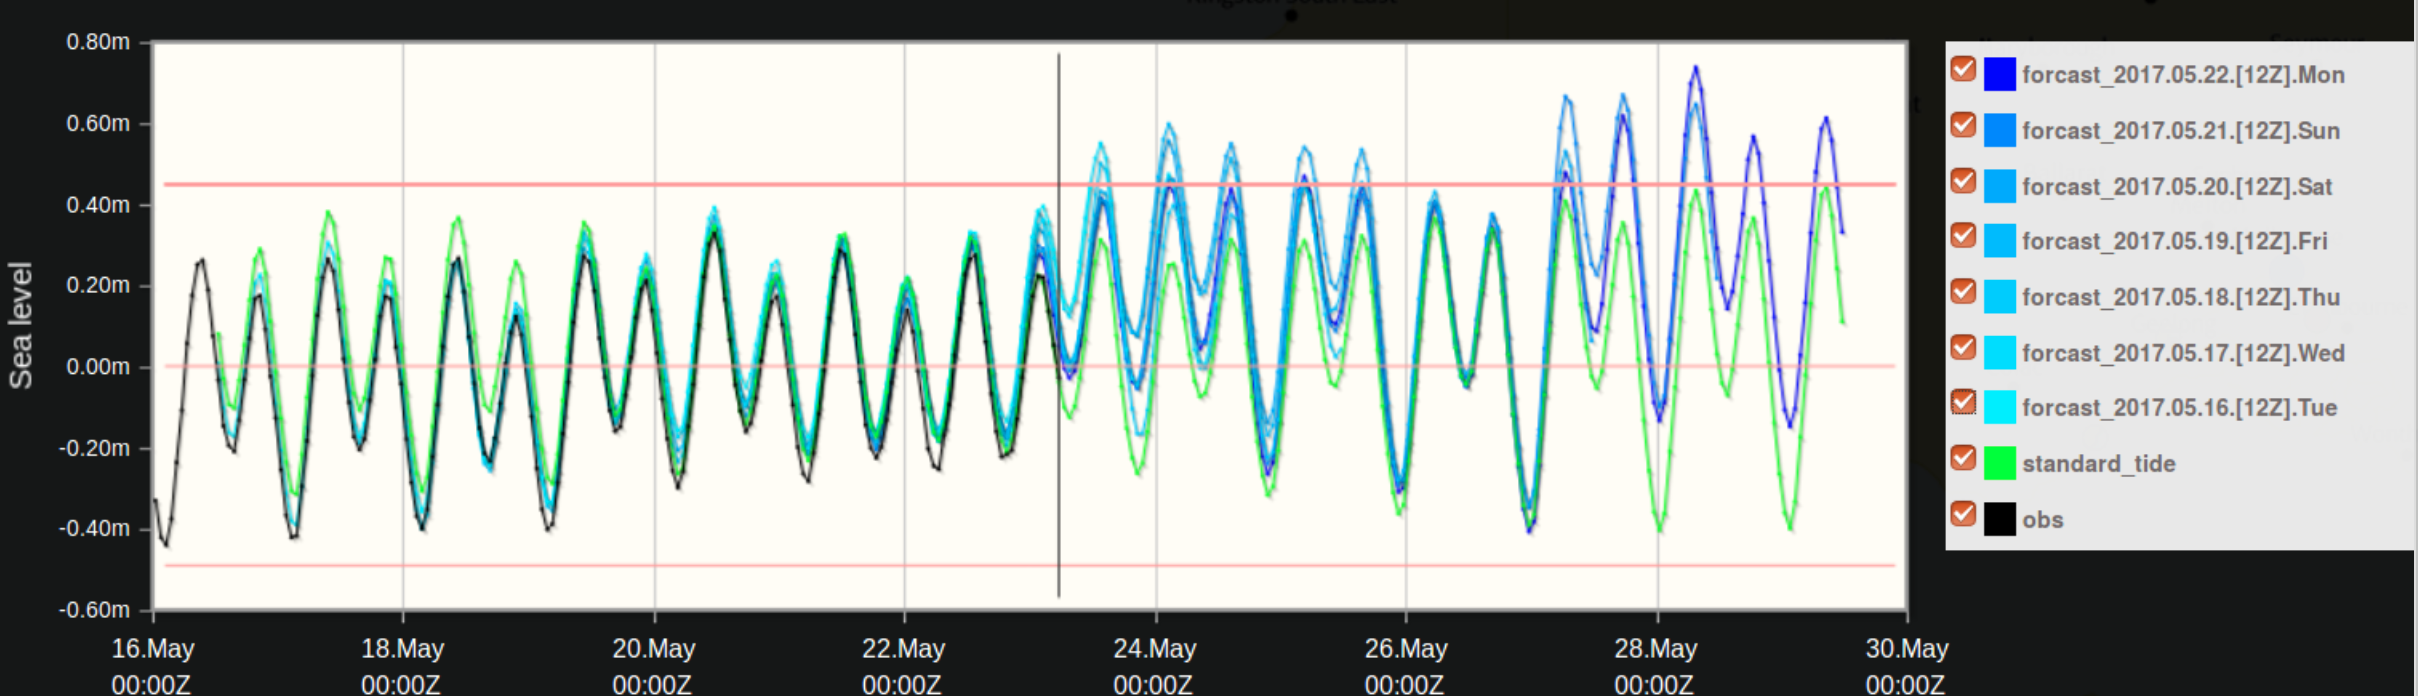
\includegraphics[width=1\textwidth]{plots/forecast_eg.png}
\caption{Illustrative sea level forecast for St Kilda at Melbourne, Australia.  Sequential 7-day forecasts are shown overlaid in shades of blue.  Observed sea level is shown in black and standard tide prediction in green.  Red horizontal lines indicate conventional tidal planes LAT, MSL and HAT.  Some spread is apparent between forecast updates.  Sea level is not especially extreme, but is forecast to cross the reference HAT in coming days.}
\label{fig:fc_eg}
\end{figure}   


%% sea level and different models 
Observed sea level is a manifestation of diverse physical processes and scales; some local in nature, but many involving signal propagation \cite{Anonymous:jdDiSHB0}.
The balance of contributions varies across the vast geographic range of the Australian coastline \cite{Haigh:2013bna,Haigh:2013hea,Woodham:2013cl,Ridgway:2004kb,Church:1986tl,Allen:2009tf}.

% evolution of targeted physical models
Specialised forecasting approaches have evolved to target different scales and subcomponents of sea level \cite{Cartwright:2000tt,Petersen:2012kp}.
A variety of systems relevant to sea level are now in side-by-side, but isolated, operation in organisations such as the Australian Bureau of Meteorology (BoM). 
These capabilities include in situ and remote observations, conventional tide predictions, wave spectra forecasts, river run-off routing and tsunami models. 
More recently, data assimilating primitive equation ocean models~\cite{Schiller:2011di} have come into operational centres via a path broadly analogous to the development of numerical weather prediction \cite{Harper:kb}. 

Inevitably the foundations of operational global forecasts are being leveraged for localised downscaled dynamic operational ocean models: e.g., \cite{Paramygin:2017dx,Yang:2016ep,Wei:2014ex,Peng:2014kq}.

However, spatial and temporal coverage is non universal; and relevance to everyday decision makers is not necessarily a direct function of increased model resolution.  


%% harmonic tides are special - data driven
\subsection{Data-Driven Conventional Tides}
\label{sec:tide_intro}

Conventional tide predictions are a remarkably successful data-driven forecast product that provides an omni-present reference for coastal activities.
By design these make no account for aperiodic phenomena. 
Production involves time series statistics based on historical records of observations at each forecast site.
Importantly, the observations need not be recently collected; let alone delivered in real time.

Tidal techniques exploit the significance of periodic sea level variations observed to be coherent with the `astronomical tide producing forces (ATGF)' \cite{Hendershott:1981ub}.     
Many variations exist for implementing this general approach (e.g., \cite{Foreman:2009bg,Groves:1975ky,LEFFLER:2009ej,Smith:1997ut} ). 
Useful sea level predictions can thereby be produced many years into the future.  
Tidal methods based on a harmonic decomposition of the ATGF have long been typical of bodies promulgating `official' tidal products; including BoM.
Official tidal products have come to have a special status; for instance, statistical properties of tidal predictions define elevation references for mapping and legal applications \cite{Mapping:2014wu}

% ...periodic but not astro 
The ongoing value of standard tidal predictions reflects the fact that periodic signals generally dominate routine coastal still water levels.
However, the physical drivers of sea level represented in tidal predictions need not be gravitational at all.
Treatment of non-gravitational signals is an practical consideration in tidal analysis proceedures; notably for the long-period constituents Sa and Ssa (\cite[]{Parker:2007wq} Sect. 3.7) but also at shorter timescales such as constituent S1 \cite{Ray:2004ts}.
The extent to which conventional harmonic tidal predictions are `physics free' actually allows for a pragmatic flexibility to represent almost all of the everyday rise and fall of coastal sea level at a place.

Even when relatively high resolution dynamic tidal models are available, the standard tide predictions at a place are commonly considered a superior estimate of routine sea level \cite{Horsburgh:2008gw,Egbert:1996vr}.


% real time insitu obs
\subsection{Real Time Observations}
Conventional tide methods have had such a long time to become deeply embedded \cite{Cartwright:2000tt} thanks to the ability to produce useful forecasts via access to observations only in a much lagged batch mode.  
In contrast, tide gauge observations are increasingly communicated in near real time to operational centres and general users. 
BoM operates its own network of tide gauges \cite{Greenslade:2012um} but the majority of available observations are shared by partner or `3rd party' organisations. 
Gathering observations from diverse organisations is valuable but can raise issues with data quality and metadata management.

Despite the nominal co-location of real-time tide gauge observations and various forecasting systems, presentation of useful verifiable guidance has been found to be surprisingly elusive.     

While more real time observations in principle opens opportunities for assimilation into dynamic models or various `trained' forecast systems \cite{Horsburgh:2011th}, such use can place much weight on the reliability and quality control of live data streams; a non-trivial concern over large regions and multiple agencies \cite{Mourre:2006hz}.


%----------------------------------------------------------------------------------------------------------------------------
\section{Forecast System Description}
\vspace{-6pt}
\subsection{Motivation}
This work is founded on the operational maturity of a global ocean forecast system (OceanMAPS) within a agency that also provides weather, tide and river forecasts.
The demonstration of limited non-tidal sea level forecast skill in earlier versions of OceanMAPS \cite{Taylor:2010ud} motivated investigation of potential practical applications. 
Liaison with forecastors and forecast-users lead to the current configuration; routine 7-day forecasts that can be directly evaluated against tide gauge observations.
A~secondary motivation was to establish a performance benchmark against which new sea level forecast capabilities can be evaluated. 

\subsection{Superposition}
\label{sec:concept}
% A generic 'one-size-fits-all' and parsimonious approach is taken.
The configuration is a linear superposition of time series derived from heterogeneous operational systems, schematically illustrated in Figure \ref{fig:aggSL} and Equation (\ref{eq:aggSL}).  
Although the superposition itself is linear, subsets of non-linear hydrodynamics are internally represented within the ocean circulation model  and the tidal harmonic fit respectively.

Component systems \textit{included} are listed here and described further below:
(1) Global ocean circulation forecasts---Section \ref{sec:dynamicmodels}, 
(2) Global numerical weather prediction---Section \ref{sec:dynamicmodels}, 
(3) adjusted harmonic tide predictions---Section \ref{sec:harmonics} and 
(4) observations-based bias correction---Section \ref{sec:bias}.

There are some notable \textit{exclusions} from the current configuration.
Spectral wave forecasts are available but not included on the basis that observation sites are located outside of surf zones (similar to  \cite{Tilburg:2004cg}).
River levels or outflow forecasts are not available in suitable form or coverage. In contrast, sea~level forecasts are an input into hydrological models \cite{Taylor:2011ud}.  

As the native time disctritisation of the input differ, each timeseries is projected onto a common 1-hourly format using an integral spline method.  
In the case of model inputs this is interpolation from 3-hourly averaged model outputs to 1-hourly.  
For observations the same method provides a~down-sampling from from 1-min or 15-min samples to 1-hourly averages.  
\begin{equation}
h(t) = \eta_{T}(t) - \eta_{HA}(t) + \eta_{SLA}(t) + \eta_{LIB}(t) + b(t0)
\label{eq:aggSL}
\end{equation}
where $h(t)$ is the aggregated sea level value at forecast time $t$.  
Signal components $\eta$ correspond to inputs in schematic Figure \ref{fig:aggSL} and subscripts $T$ and $HA$ indicate tide and harmonic adjustment respectively.    
Bias correction $b$ is a fixed value across each forecast.
\vspace{6pt}
\begin{figure}[H]
\centering
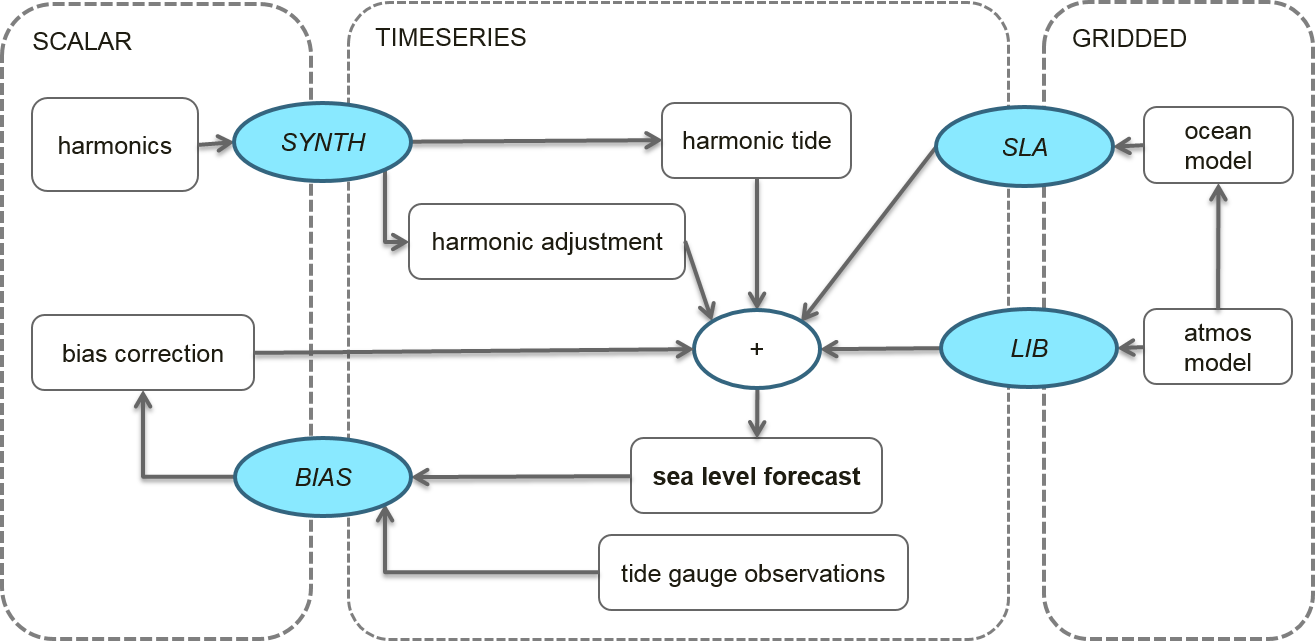
\includegraphics[width=1.0\textwidth]{plots/aggSL_schematic_abstract.png}
\caption{Schematic illustration of aggregation configuration.  Source systems are heterogeneous but mapped onto time series that can be directly compared against 1-hourly observations.  (\textbf{SYNTH}) indicates tidal synthesis, (\textbf{SLA}) sea level anomaly from OceanMAPS, (\textbf{LIB}) local inverse barometer approximation based on atmospheric pressure forecast, (\textbf{BIAS}) non-causal filter bias correction scheme. }
\label{fig:aggSL}
\end{figure}   



% INPUT - oceanmaps and access
\subsection{ Input: Data Assimilating Primitive Equation Forecasts }
\label{sec:dynamicmodels}

Near-global ocean forecasts have been in operational production at the BoM now for 10 years via several versions of the Ocean Model, Analysis and Prediction System (`OceanMAPS')~\cite{Brassington:2007ut,NMOC:2007wq,BureauofMeterology:2011ta,Brassington:2012wm}.
The~dynamic ocean model component of OceanMAPS is based on the Modular Ocean Moel (`MOM')~\cite{Griffies:2008vh} configured with 0.1 $\times$ 0.1 degree regular structured horizontal resolution, hydrostatic free surface, z-level and split-implicit scheme; where the barotropic calculation is performed at a finer time stepping. 

Gravitation tidal forces are intentionally \textit{not} included in OceanMAPS.      


Land run-off fresh water fluxes are only roughly approximated with a climatological annual cycle. 
Australian rivers are typically dry for very long periods with intermittant flooding.   
The climatological river input is only included for maintaining global mass balance and has essentially no skill for Australian river outflow impacts on sea level.    


Initial conditions for the ocean state are constrained using an ensemble optimal interpolation data assimilation scheme \cite{Oke:2008wr} which ingests a large number and range of remote and in situ ocean observations. 
Importantly for sea level, tide gauge observations are \textit{not} assimilated and are independent.   
Satellite altimeter observations of sea level are assimilated, but not inshore of the shelf break; nominally cut off at the 200 m isobath.


Atmospheric fluxes, excluding barometric pressure, are applied directly from the global numerical weather prediction (NWP) system ACCESS-G \cite{BureauofMeterology:C8IaJ2Qq}.
ACCESS-G is also based on a data assimilating primitive equation model.
It is not coupled with any ocean model beyond use of a persisted SST analysis boundary condition.
These flux fields are generated on a N512 gaussian grid with an indicative spatial resolution of~25 km. 
% (The NWP forecast fluxes extend for 10-days.)

OceanMAPS produces a new ocean state forecast each day for the next 7-days using a multi-cycle ensemble schedule \cite{GaryBBrassington:2013jw}.

As a result, 7-day forecasts of a sea level anomaly ($\eta_{SLA}$) quantity are reliably available each day.  
This data is output as 3-hourly averages.  
The quantity $\eta_{SLA}$ is not directly observable, but in the open water is observationally constrained by corrected altimeter observations.
$\eta_{SLA}$ is quantified relative to the model rest state, which nominally represents a geopotential surface like mean sea level.  

The regular spatial discretisation of OceanMAPS does not resolve features smaller than 10 km.   
And some nominally larger embayments have been intentionally excluded; such as Port Phillip Bay in South Eastern Australia.
The Arakawa B-grid discretization imposes a numerical requirement to exclude 1-cell bays. 
An minumum depth of three z-levels equivalent to 15 m is also imposed.

The representation of the coast is illustrated in Figure \ref{fig:map_masks}.

In order to map the gridded $\eta_{SLA}$ field to a tide gauge location, a generic one-to-one `nearest coastal neighbour' algorithm is applied.
A manual exception for cell selection is applied to the Port Phillip case to ensure alignment with the single bay entrance. 
\vspace{6pt}
\begin{figure}[H]
    \centering
    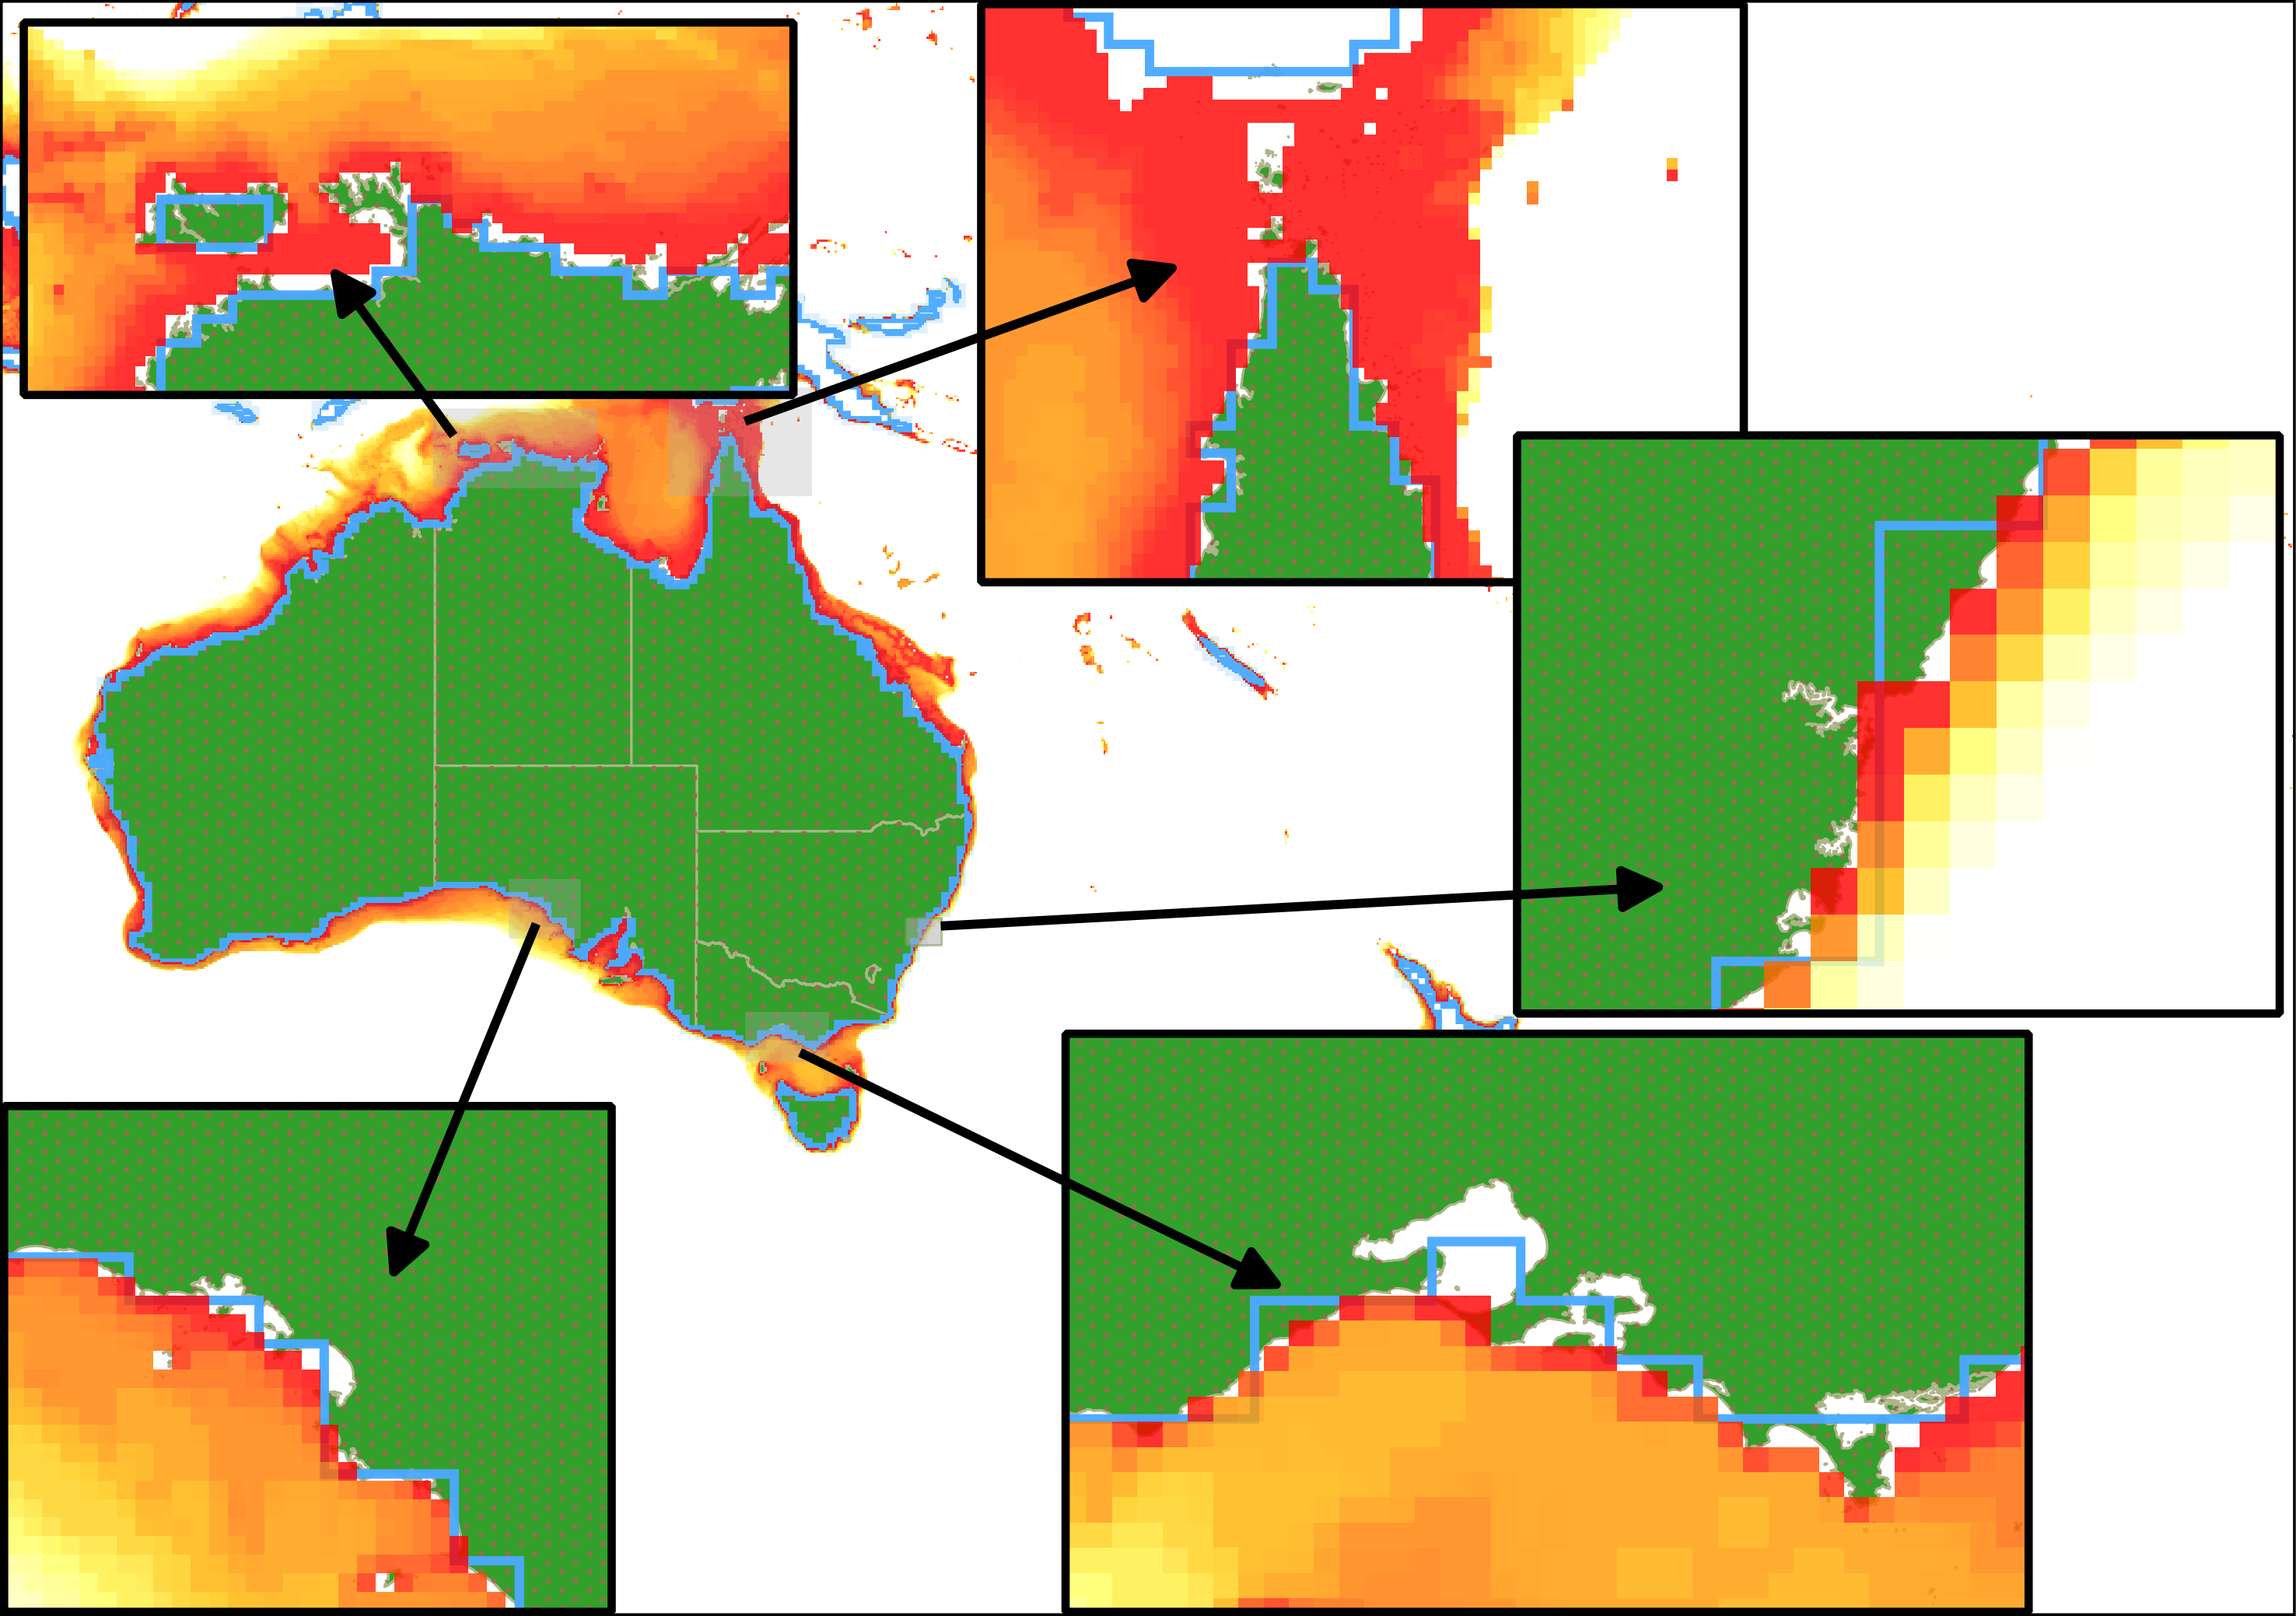
\includegraphics[width=1.0\textwidth]{plots/omaps_masks.png}
    \caption{Illustration of coastal discretisation.  Red coloured grid cells indicate ocean model bathymetry the inner extent of which is the model coastline.  The thick blue line indicates the edge of the atmospheric model land/sea mask.  Most small scale features and embayments at tide gauge locations are only approximated at scales above~10 km in the ocean and~80 km in the atmosphere. }
    \label{fig:map_masks}
\end{figure}  


OceanMAPS does not represent the effect of atmospheric pressure forces on the ocean.
Subsequently, a local inverse barometer approximation is applied as per Equation (\ref{eq:lib}).
This formulation was chosen for being simple and robust, but is acknowledged as a compromise with regard to atmospheric representation and non-instantaneous ocean responses \cite{Mathers:2004bk}.
A fixed conventional reference pressure, rather than one derived from the NWP, was considered appropriate given the generic offset adjustment built into the bias correction scheme (Section \ref{sec:bias}).  
\begin{equation}
  \eta_{LIB} = \frac{ p_{NWP} - p_{ref} }{ \rho g }
  \label{eq:lib}
\end{equation}
where reference pressure is fixed at $p_{ref}$ = 101,325 Pa, and bulk sea water density is also kept fixed at 1027 $\text{kg}/\text{m}^3$.
Only a small subset of tide gauges are co-located with real-time barometer instruments.


\subsection{Input: Tidal Harmonics }
\label{sec:harmonics}
Officially promulgated tide predictions have a special relevance, as raised in Section \ref{sec:tide_intro}.
The~aggregation configuration intentionally aims to align with the BoM's existing tide tables. 

However, the heterogeneous nature of harmonic tide analysis and OceanMAPS configuration leads to a situation where the respective sea level signals are not cleanly complimentary.
In particular some of the sea level variation in the ocean model may be seen as `tidal', whereas some of the variation in the tidal harmonics may be seen as meteorological.   
In isolation, this spectral overlap is generally not problematic. 
However, linear superposition of the OceanMAPS $\eta_{SLA}$ with standard tides can lead to undesirable double-counting. 
This is most obvious at longer time scales in Northern Australia; where relatively powerful seasonal sea level changes have projected onto tidal harmonics.


A pragmatic approach is taken that aims to address both of these motivations; namely to align with other official tidal products and mitigate effects of spectral overlap.
The BoM's operationally supported tidal synthesis software is applied to two versions of tidal harmonics for each location:
\begin{itemize}[leftmargin=*]%,labelsep=5.8mm]
  \item full set of tidal harmonics: typically 114 constituents.
  \item subset assigned apriori to be primarily non-gravitational in expression: Sa, SSa, Mm, Msf and S1.
\end{itemize}

The subset time series is designated as a harmonic adjustment signal that is then subtracted within the superposition of signals. 


\subsection{Input: Bias Correction}
\label{sec:bias}
Near real-time observations are available at an increasing number of tide gauge locations, and~intuitively serve as a source of guidance to users.
Typical practice, though often not formalised, is~to~inspect recent tidal error (residual) evolution and project as a correction to tide tables into the near~future.

Operational availability of this source of information is exploited in a generic and un-trained bias correction scheme. 
The bias term ($b$ in Equation (\ref{eq:aggSL})) is a constant added to each forecast.
The value of $b$ is derived as a weighted mean of recent errors between observed sea level and previous forecasts between 0--24 lead times.
The most recent value persists in the case of observation drop-outs and gaps.
Observations are pre-processed with a median spike filter to mitigate the impact of communications glitches and noise.
Weighting is tapered such that the influence of older error values decreases with time prior to the present and it is `causal' in the sense that no observations after the forecast base time have any influence.
The total window length of the filter spans 21 days.
Identical settings are applied to all locations.


The scheme aims to cover multiple needs.
Firstly, to address alignment of reference datums between sources. 
It is the temporal evolution of $\eta_{SLA}$ and $\eta_{LIB}$ that is expected to contain real information---not the absolute values.
Moreover, metadata ambiguity with regard to the reference datum of real-time observational streams (from 3rd parties) relative to tide prediction datums has proven to be a real issue.
Secondly, the correction serves as a crude data assimilation method to adjust the vertical offset of the forecast in light of long period error evolution. 

The actual behaviour of this term is discussed further in Section \ref{sec:bias_more}.

%----------------------------------------------------------------------------------------------------------------------------
\section{Evaluation}

Evaluation results are presented based on aggregate sea level forecasts produced in an operational mode at BoM between June 2016 to May 2017.

\subsection{Geographic Overview}
Evaluation is restricted to a series of point locations.  These locations correspond to tide gauges from which real-time information was reported into the operational centre over the study period.  An overview map of these locations is shown in Figure \ref{fig:map_locations}.
The inconsistent coastal distance between locations is an outcome of human population distribution and inter-organisational arrangements.
It~is~foreseeable that the number of sites could expand significantly in the future.
\vspace{6pt}
\begin{figure}[H]
    \centering
    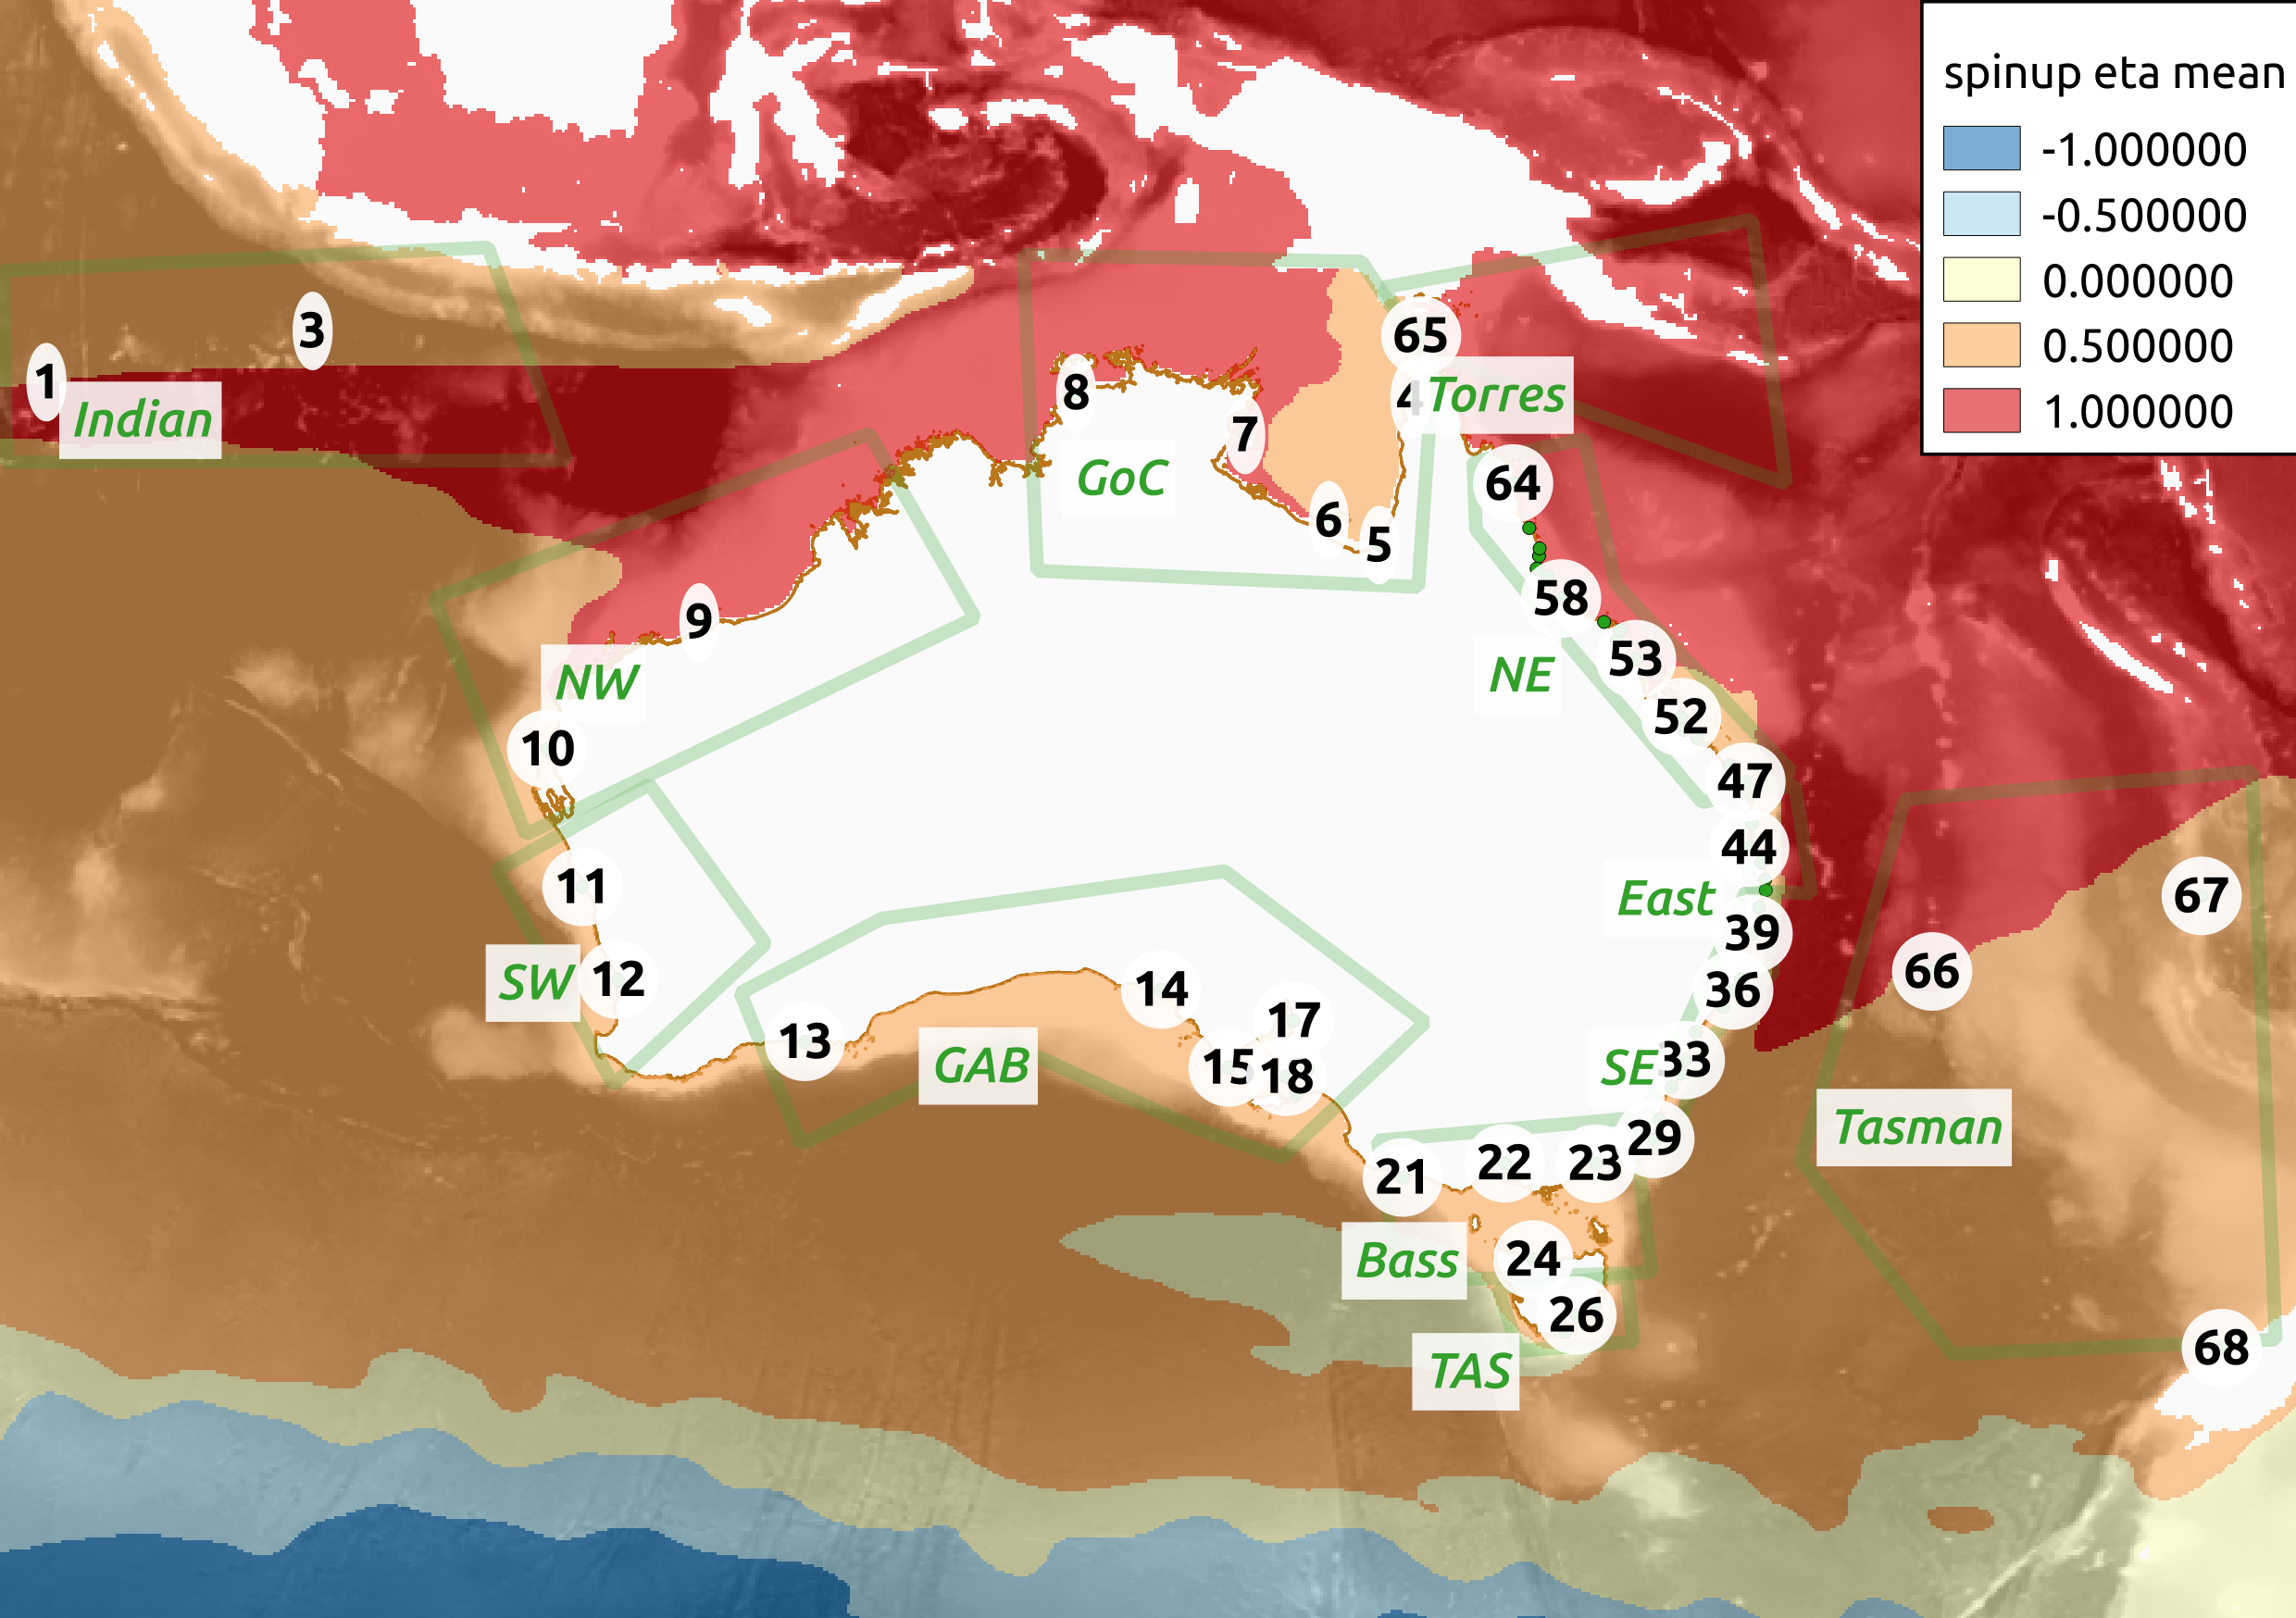
\includegraphics[width=1.0\textwidth]{plots/omaps_bathy_and_eta.png}
    \caption{Geographic overview of Australia region.  Ocean model bathymetry is indicated by grey background shading.  Colour contours illustrate the `spin up' model mean dynamic topography referenced below.  Tide gauge locations are identified with sequential numbers with order chosen to loosely align with anti-cyclonic coastal wave propagation direction. Regional groupings are referenced in subsequent results.}
    \label{fig:map_locations}
\end{figure}  

The observation locations are quite diverse with regard to exposure to the open ocean, instrumentation, sample frequency and communications quality. 


\subsection{Forecast Goodness as Routine Guidance}
In general, forecast goodness cannot be properly judged against any single measure.
The~evaluation below is informed by the the concepts of `quality' and `value' following Murphy~\cite{Murphy:1993dh}.
Even if the component parts contain comparative technical deficiencies, the whole package may offer real value above available alternatives.
For this routine guidance use-case, only full time series statistics are presented as an evaluation. 
Categorical and event-based measures are not addressed in this paper.


Harmonic tide predictions considered in light of recent residuals commonly offer remarkably good guidance for coastal sea level.
Such a `tide + persisted residual' scheme is formulated in Equation~(\ref{eq:tide_res}) and taken as an appropriate benchmark against which to evaluate the aggregated forecast.
For~the new scheme to offer value at a particular location it must demonstrate superior skill relative to this~benchmark.  
\begin{equation}
h_{T+r}(t) = \eta_{T}(t) + r(t0)
\label{eq:tide_res}
\end{equation}

Following Equation (\ref{eq:aggSL}) where $r(t0)$ is the difference between observations and tide prediction $\eta_{T}$ at or just prior to forecast base time. 

\subsection{Highlighted Behaviour}
The time series shown in Figure \ref{fig:ts_melb} is included as an example of a skilful dynamic model contribution.  
This location is subject to relatively powerful sea level variations associated with mid-latitude weather.
Of interest is the fact that the embayment in which the observations are taken is not represented at all in the ocean model.  This indicates the large influence of sea level outside of the bay at these timescales. 

\begin{figure}[H]
    \centering
    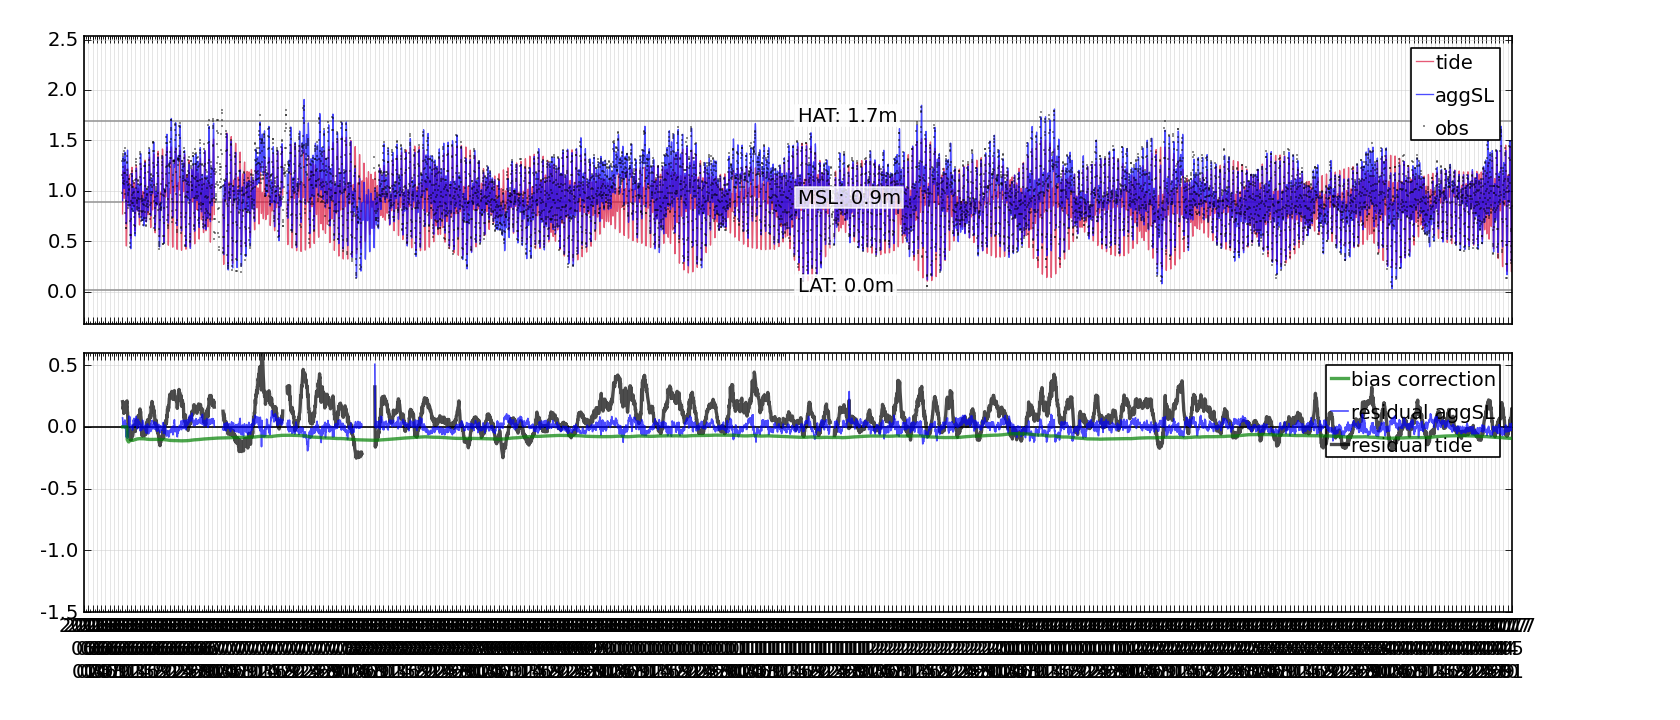
\includegraphics[width=\textwidth]{plots/0026_plot_timeseries.png}
    \caption{ Example time series record for location at Melbourne (\textbf{23} in Figure \ref{fig:map_locations} ); Upper panel shows total still water levels relative to conventional tidal benchmarks. Lower panel shows error signals and bias correction evolution.  Errors (`residuals') are shown overlaid for standard tides and aggregate forecasts (`aggSL') categorised by forecast lead time;  each continuous aggSL timeseries is concatenated from forecast lead times of 0--24 h (aggSL0), 24--48 h (aggSL1), ... , 144--168 h (aggSL6).  An~overall reduction in error variance is apparent between standard tides and aggregate forecasts; errors grow with forecast lead time.   
    Large reduction in error variance relative to harmonic tides is evident.}
\label{fig:ts_melb}
\end{figure}   


Contrasting behaviour is illustrated in Figures \ref{fig:pdf} and \ref{fig:rms} by means of error statistics.
At all three locations the aggregated forecasts offer `quality' in the sense of matching observations; but for different reasons and different degress of potential value. 

\begin{figure}[H]
    \centering
    \begin{subfigure}{0.30\textwidth}
    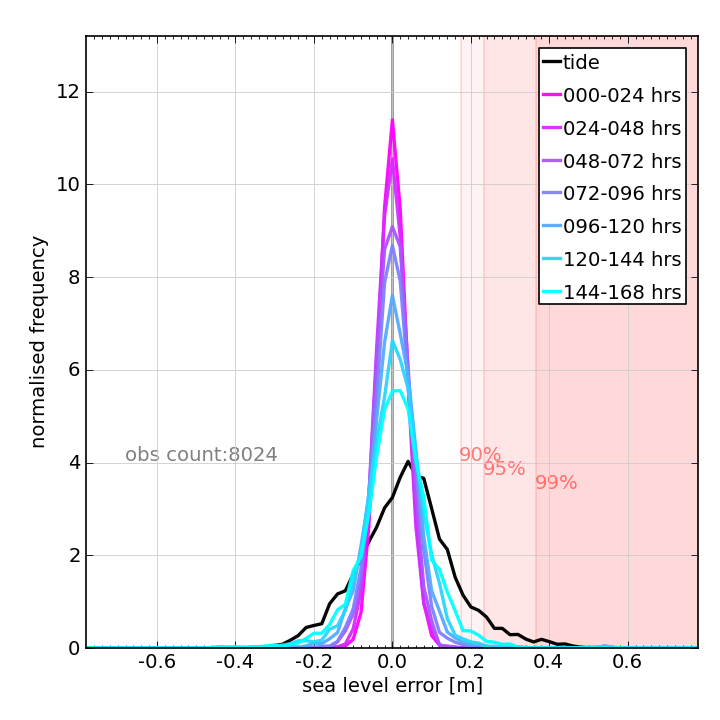
\includegraphics[width=0.9\textwidth]{plots/0013_verify_pdf.png}
    \caption{}
    \end{subfigure}
    \begin{subfigure}{0.30\textwidth}
    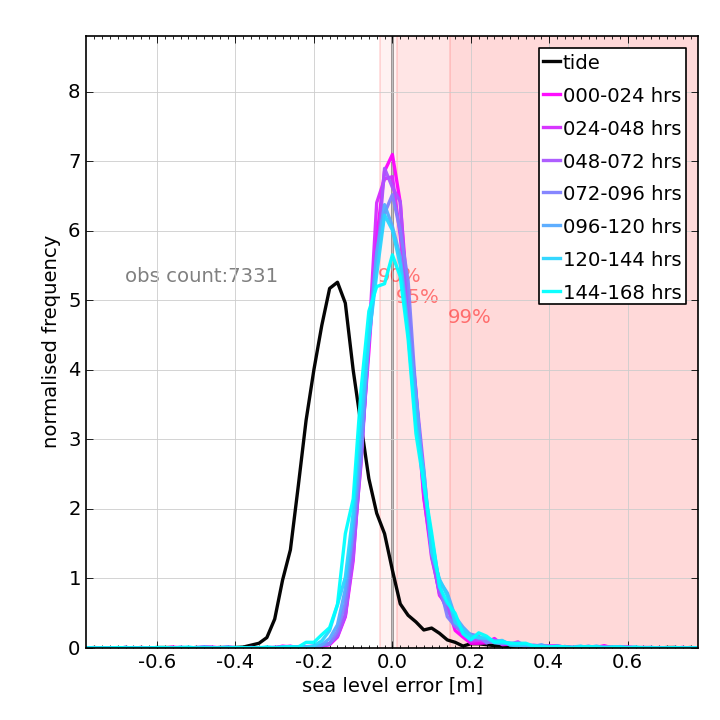
\includegraphics[width=0.9\textwidth]{plots/0043_verify_pdf.png}
    \caption{}
    \end{subfigure}
    \begin{subfigure}{0.30\textwidth}
    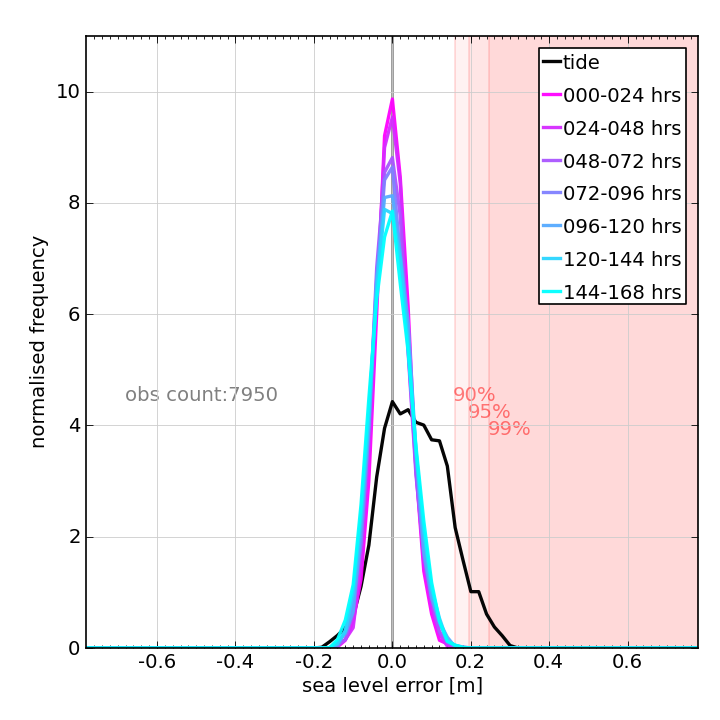
\includegraphics[width=0.9\textwidth]{plots/0003_verify_pdf.png}
    \caption{}
    \end{subfigure}
    \caption{ Forecast error distributions at selected contrasting locations. Skill improvement over standard harmonic tides is driven by different aspects of the generic aggregation process. (\textbf{a}) shows skill gain due to forecast signals associated with mid-latitudee weather (\textbf{b}) shows the practical problem of mismatched reference datums between real-time observational data and tide predictions (see Section~\ref{sec:bias_more}), (\textbf{c}) is a location at which longer period deviations from tide predictions are relatively powerful. (\textbf{a}) Site 13, Mid-latitude weather; (\textbf{b}) Site 43, Tide datum mismatch; (\textbf{c}) Site 3, Long period anomalies.}\vspace{-17pt}

    \label{fig:pdf}
\end{figure}   


\begin{figure}[H]
    \centering
    \begin{subfigure}{0.30\textwidth}
    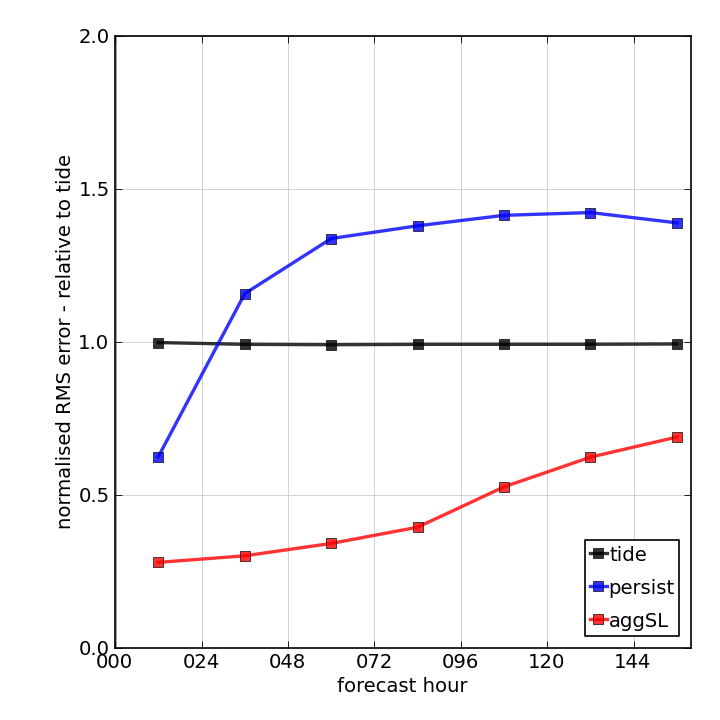
\includegraphics[width=0.9\textwidth]{plots/0013_rms_growth.png}
    \caption{}
    \end{subfigure}
    \begin{subfigure}{0.30\textwidth}
    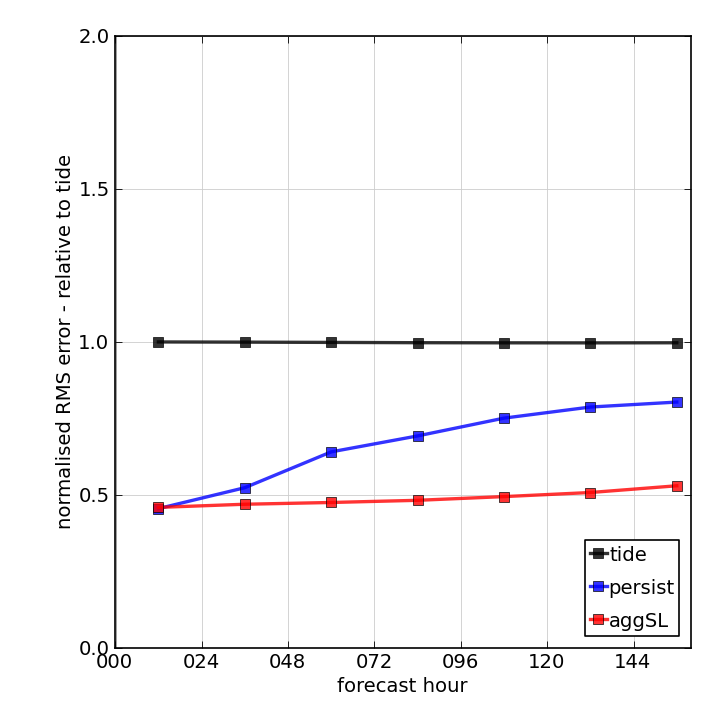
\includegraphics[width=0.9\textwidth]{plots/0043_rms_growth.png}
    \caption{}
    \end{subfigure}
    \begin{subfigure}{0.30\textwidth}
    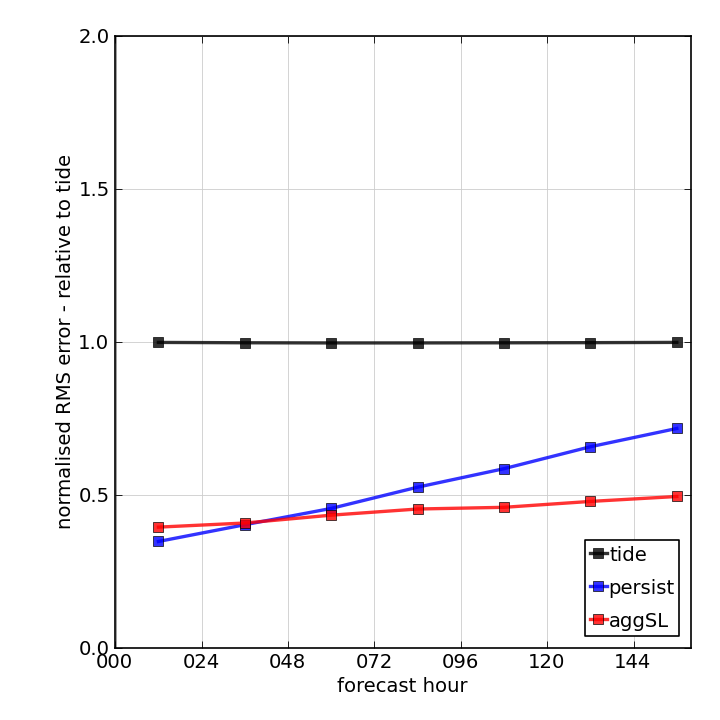
\includegraphics[width=0.9\textwidth]{plots/0003_rms_growth.png}
    \caption{}
    \end{subfigure}
    \caption{ Relative error metrics at select locations as per Figure \ref{fig:pdf}. RMSE at increasing forecast lead times is normalised and plotted relative to the standard tidal residual---such that a lower value represents greater accuracy. Error growth with forecast age is evident. (\textbf{a}) As per (a) in Figure \ref{fig:pdf}; (\textbf{b}) As per (b) in Figure \ref{fig:pdf}; (\textbf{c}) As per (c) in Figure \ref{fig:pdf}.} \vspace{-13pt}
    \label{fig:rms}
\end{figure}   

\subsection{Skill Summary: Non-Tidal Information Decay}
\label{sec:skill}

In order to highlight the differentiation between dynamic forecast skill between locations, Figure~\ref{fig:taylors} summarises average forecast evolution characteristics using Taylor diagrams \cite{Taylor:2000wp} for time series that have been de-tided using a band-limited harmonic tide.
Each `comet' contains a point for each 24~h period of the 7-day forecasts.
Site number is located at the 1st day forecast point.
Both the reference observations and forecasts have been de-tided using only the nominally gravitational tide signal described in Section \ref{sec:harmonics}.
All statistics are centered and normalised relative to the reference observation value $\hat{h}_{OBS}$ as defined in Equation (\ref{eq:taylor}).
\begin{equation}
\begin{split}
\hat{h}_{OBS}(t) &= h_{OBS}(t) - (\eta_{T}(t) - \eta_{HA}(t))  \\ 
\hat{h}_{FC}(t)  &= \eta_{SLA}(t) + \eta{LIB}(t) + b(t0) 
\label{eq:taylor}
\end{split}
\end{equation}

Following Equation (\ref {eq:aggSL}).  Where $\hat{h(t)}$ is sea level de-tided using a band-limited tidal time series.  





\begin{figure}[H]
\vspace{-10pt}
\centering
    %------ 1
    \begin{subfigure}{0.30\textwidth}
        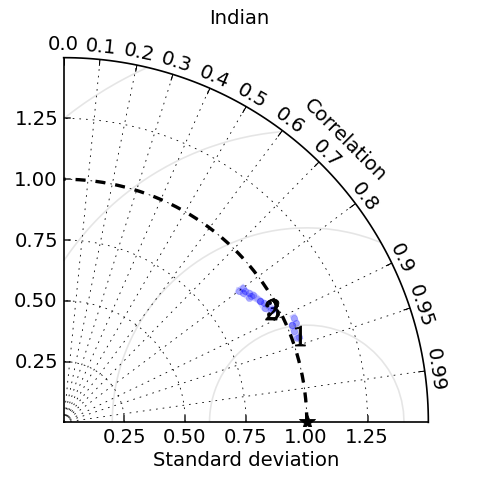
\includegraphics[width=\textwidth]{plots/taylor_diag_res_Indian.png}
        \caption{}
    \end{subfigure}
    \begin{subfigure}{0.30\textwidth}
        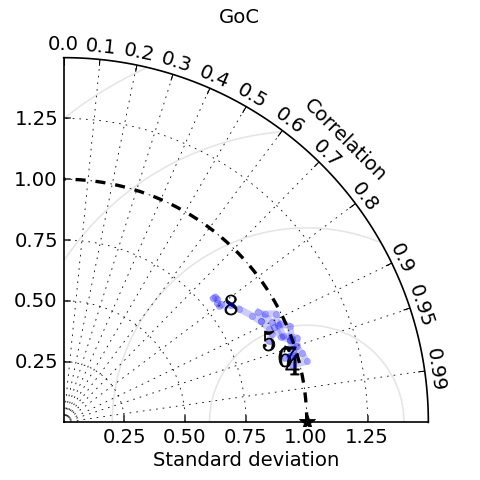
\includegraphics[width=\textwidth]{plots/taylor_diag_res_GoC.png}
        \caption{}
    \end{subfigure}
    \begin{subfigure}{0.30\textwidth}
        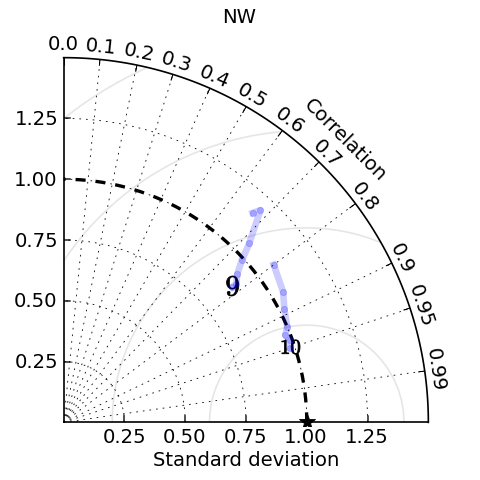
\includegraphics[width=\textwidth]{plots/taylor_diag_res_NW.png}
        \caption{}
    \end{subfigure}
    %-------2
  \begin{subfigure}{0.30\textwidth}
     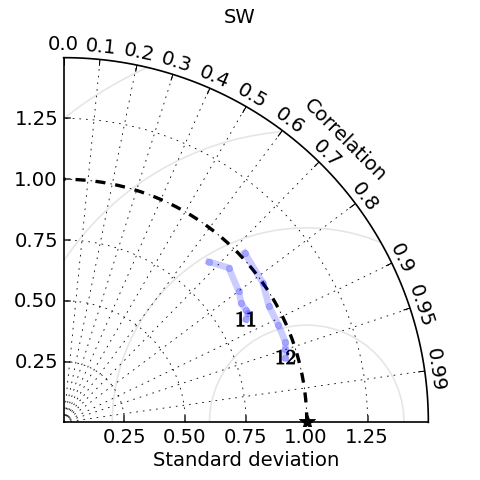
\includegraphics[width=\textwidth]{plots/taylor_diag_res_SW.png}
        \caption{}
    \end{subfigure}
    \begin{subfigure}{0.30\textwidth}
        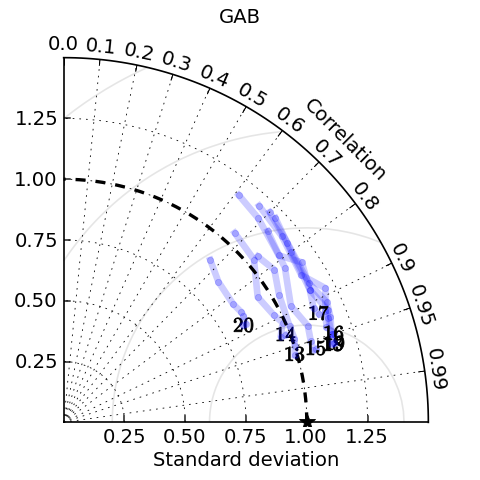
\includegraphics[width=\textwidth]{plots/taylor_diag_res_GAB.png}
        \caption{}
    \end{subfigure}
    \begin{subfigure}{0.30\textwidth}

        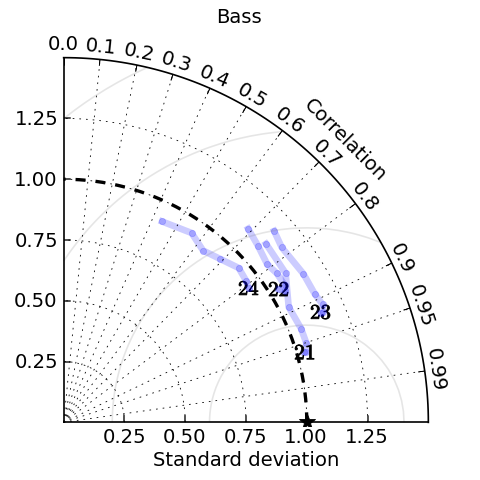
\includegraphics[width=\textwidth]{plots/taylor_diag_res_Bass.png}
        \caption{}
    \end{subfigure}
    %-------3
    \begin{subfigure}{0.30\textwidth}
          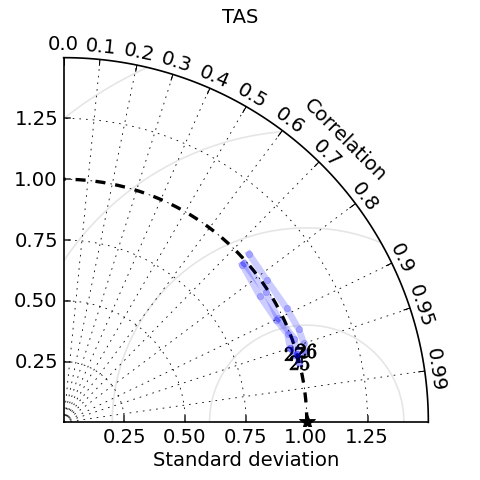
\includegraphics[width=\textwidth]{plots/taylor_diag_res_TAS.png}
        \caption{}
    \end{subfigure}
    \begin{subfigure}{0.30\textwidth}
        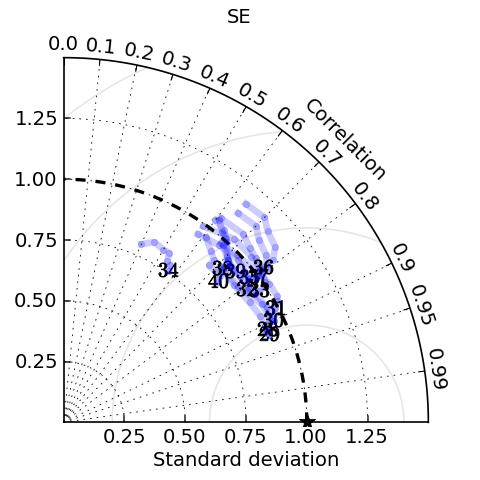
\includegraphics[width=\textwidth]{plots/taylor_diag_res_SE.png}
        \caption{}
    \end{subfigure}
    \begin{subfigure}{0.30\textwidth}
        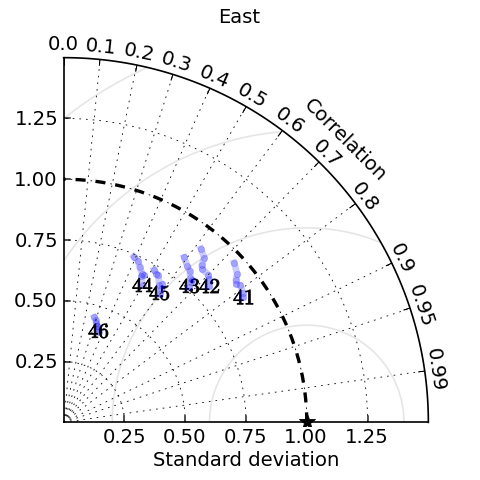
\includegraphics[width=\textwidth]{plots/taylor_diag_res_East.png}
        \caption{}
    \end{subfigure}
    %-------4
    \begin{subfigure}{0.30\textwidth}
        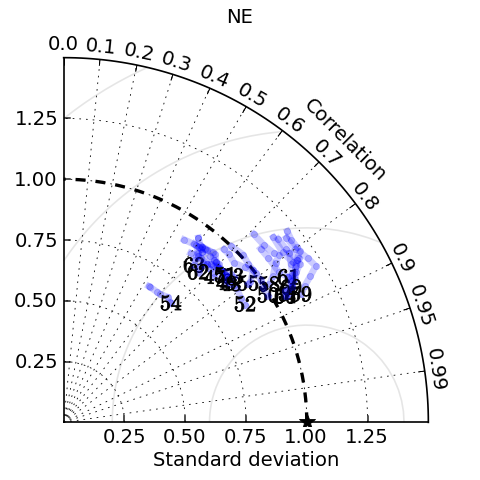
\includegraphics[width=\textwidth]{plots/taylor_diag_res_NE.png}
        \caption{}
    \end{subfigure}
    \begin{subfigure}{0.30\textwidth}
        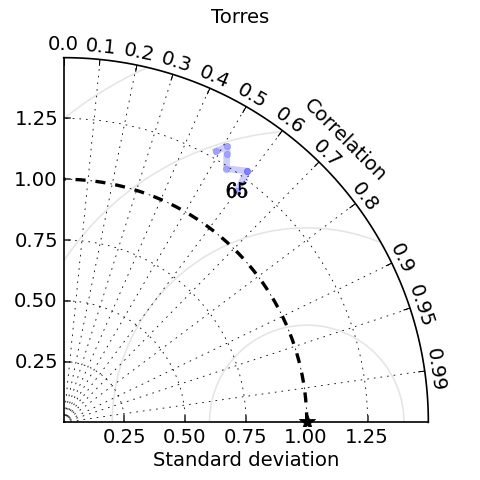
\includegraphics[width=\textwidth]{plots/taylor_diag_res_Torres.png}
        \caption{}
    \end{subfigure}
    \begin{subfigure}{0.30\textwidth}
        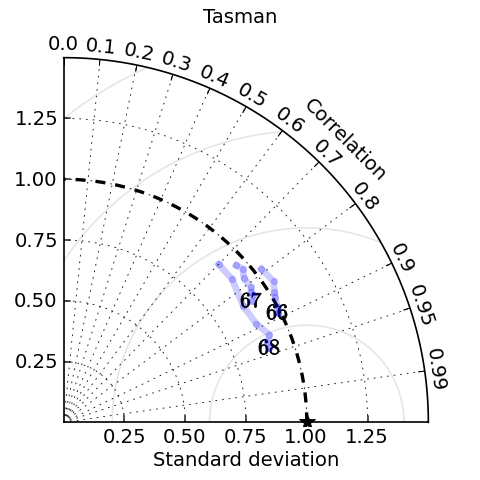
\includegraphics[width=\textwidth]{plots/taylor_diag_res_Tasman.png}
        \caption{}
    \end{subfigure}
    %--------
    \caption{ Taylor diagrams summarising dynamic skill evolution across 7-day forecasts.
    Each `comet' describes average statistics for one location.
    Panels are divided according to regions shown in Figure~\ref{fig:map_locations}.
    Statistics are derived from filtered time series, not total sea level, and are normalised relative to the reference observations. (\textbf{a}) Indian; (\textbf{b}) Gulf of Carpentaria; (\textbf{c}) North West; (\textbf{d}) South West; (\textbf{e}) Great Aust Bight; (\textbf{f}) Bass Strait; (\textbf{g}) Tasmania; (\textbf{h}) South East; (\textbf{i}) East; (\textbf{j}) North East; (\textbf{k}) Torres Stait; (\textbf{l})~Tasman Sea. }\vspace{-12pt}
    \label{fig:taylors}
\end{figure}   
A notable feature of this visualisation is the de-correlation with forecast lead time.   
This is expected behaviour of a skillful deterministic forecast model where errors grow due to explicit numerical approximation of chaotic dynamics. 
Regional differences are apparent in degree of initial correlation and rate of de-correlation.

The under-prediction of variability in the `East' region (panel i) appears to reflect the noisy observational data streams from these 3rd party sites - such that the observation reference variability is inflated by communications glitches.

Anomalous variability growth for station 9 in `NW' region (panel c) was found to reflect the influence of a small number of over-forecast tropical cyclone events.  While the resolution limitations of the atmospheric forcing rule out applicability to extreme storm surge forecasts, NWP systems do evolve TCs that subsequently drive sea level signals in the OceanMAPS. In this case, the relative size of these over-forecasts at longer lead times is reflected in the Taylor diagram `comet'.

Torres Strait stands out for general poor performance and will be the subject of future~investigation.



\subsection{Skill Summary: Comparison Against `Tide + Persisted Residual'}
Based on the relative RMSE evaluation shown in Figure \ref{fig:rms} a traffic-light summary map of results is shown in Figure \ref{fig:map_rms}.
A red symbol indicates that aggregated forecast RMSE score is lower (better) than that of the reference `tide + persisted residual' for the specified forecast lead time, a blue symbol indicates the opposite.  Where neither is better than standard tides, a black symbol is allocated.   
\begin{figure}[H]
    \centering
    \begin{subfigure}[b]{0.45\textwidth}
        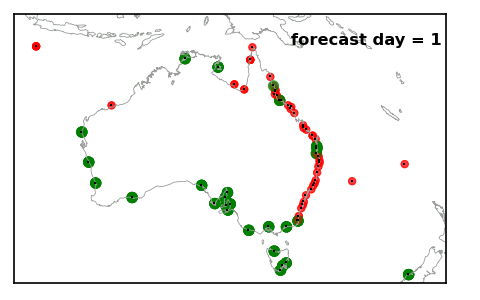
\includegraphics[width=\textwidth]{plots/plot_map_rms_score_day_1.png}
    \end{subfigure}
    \begin{subfigure}[b]{0.45\textwidth}
        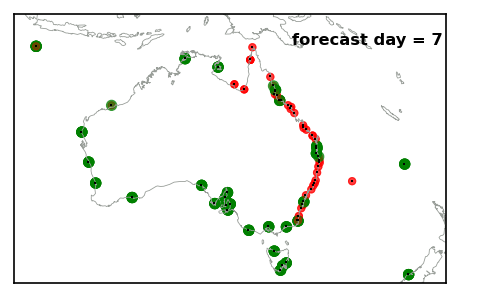
\includegraphics[width=\textwidth]{plots/plot_map_rms_score_day_7.png}
    \end{subfigure}
    \caption{ Summary map showing which forecast source provides best information on average with regard to RMS error reduction. Red symbols at locations where aggregated forecast is best, blue for `tide + persisted residual' and black for standard tides.  Forecast lead times of 0--24 h are shown in left panel, and 144--168 h on the right.}
    \label{fig:map_rms}\vspace{-3pt}
\end{figure}   



%-------------------------------------------------------------------------
\section{Role of Bias Correction Component}
\label{sec:bias_more}

The practical behaviour of the bias correction term is of special interest for evaluation.   
It is the only data driven term allowed to evolve in operations as described in Section \ref{sec:bias}.
An example time series is shown in the lower panel of Figure \ref{fig:ts_melb}.
The relatively static nature is typical of other sites.


To characterise behaviour each bias correction record was decomposed into a mean and temporarily varying signal.

%% mean
The mean bias correction is primarily aligned with the ocean model representation of mean dynamic topography MDT (compare \cite{Slobbe:wk}).
Such a reference surface in model space is the most common strategy used in the assimilation of altimetry observations, which are themselves constructed as anomalies from a reference surface in observation space. For OceanMAPS this surface was derived from a long free `spin up' run of the model \cite{Oke:2013fm}. 
Figure \ref{fig:bias_mean} shows the correspondence between model MDT ($\eta_{spinup}$) and the \textit{negative} of the bias correction mean.   The wider spatial distribution of MDT is indicated by contours in Figure \ref{fig:map_locations}.

\begin{figure}[H]
\centering
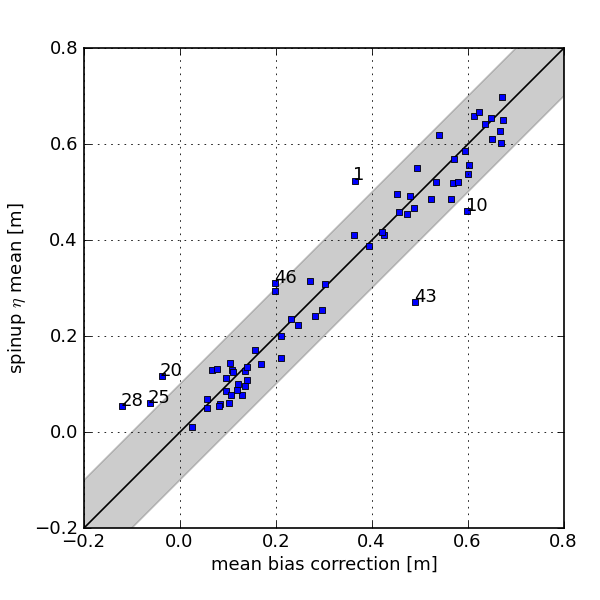
\includegraphics[width=0.5\textwidth]{plots/aggSL_bias_breakdown_plot_1.png}
\caption{ Magnitude of the temporal mean of bias correction matched against model MDT surface at each location. An arbitrary mismatch threshold of 10 cm is used to highlight apparent outliers.}\vspace{-6pt}
\label{fig:bias_mean}
\end{figure}   

As the model MDT is known apriori, this correspondance supports the expectation that it is a~good first guess of the bias term.

Several sites deviate from this alignment by more than a fixed arbitrary threshold of 10 cm, and~these are distributed across the domain.
% This simple metric does not account for the wide range of signal variance around the coast. 
A large deviation indicates that the bias correction term systematically adjusted for information not available in the modeling systems alone.  


Site 46 is an esturine location where observations are strongly effected by surrounding sand sediment. The bias term at this location is partially adjusting to the asymmtery of the choked tidal~signal. 


Model sources of bias are feasible and likely.
However, of special note is the possibility of datum metadata mismatch between the available real-time observation data stream and the standard tide predictions. 
Site 43 is an example of a 3rd party datastream with such~a~mismatch. 

This is a symptom of organisational rather than modeling factors.   
Australian tide gauges are owned and operated by different bodies under a variety of data sharing arrangements.
Consistent metadata management from these diverse agencies remains problematic, despite being a nominally simple matter.

Tide predictions in Australia are reported relative to `prediction datum' which \textit{typically} aligns with the promalgated lowest astronomical tide (LAT) value.   
From time to time either the value for LAT or the alignment of prediction datum may be updated.  
% Real-time observations may have become available within the operational centre for reasons other than tide monitoring; in particular when such data is collated with river flood warning information.  
While overall the real-time data is expected to be reported relative to either instrument zero, Australian Height Datum (AHD) or tidal prediction datum, operational systems avaiable at the time of writing cannot reliably manage these differences.
% 1   200865   Cocos
% 10  6108     Cape Cuvier 
% 20  523757   Cape Jervis SA
% 25  94243    South port TAS
% 28  69129    TwoFold NSW
% 43  40881    AirSea at QLD << used in example
% 46  540311   Nooosa bar ... sedimentation within sand bar , low value clips


%% temporal
The temporally varying bias correction signals for each station are arranged in numbered order in Figure~\ref{fig:bias_time}.
Column order is such that adjacent stations are together, though separation distance varies greatly. 
In this visualisation it is apparent that the time varying signal has relatively small amplitude of~$<$7 cm for the majority of sites.
The single station located Torres Strait is a stand-out exception.  The~sea level signal at this location is the subject of further investigation, but for the present purpose will be disregarded as not valid.  


\begin{figure}[H]
\centering
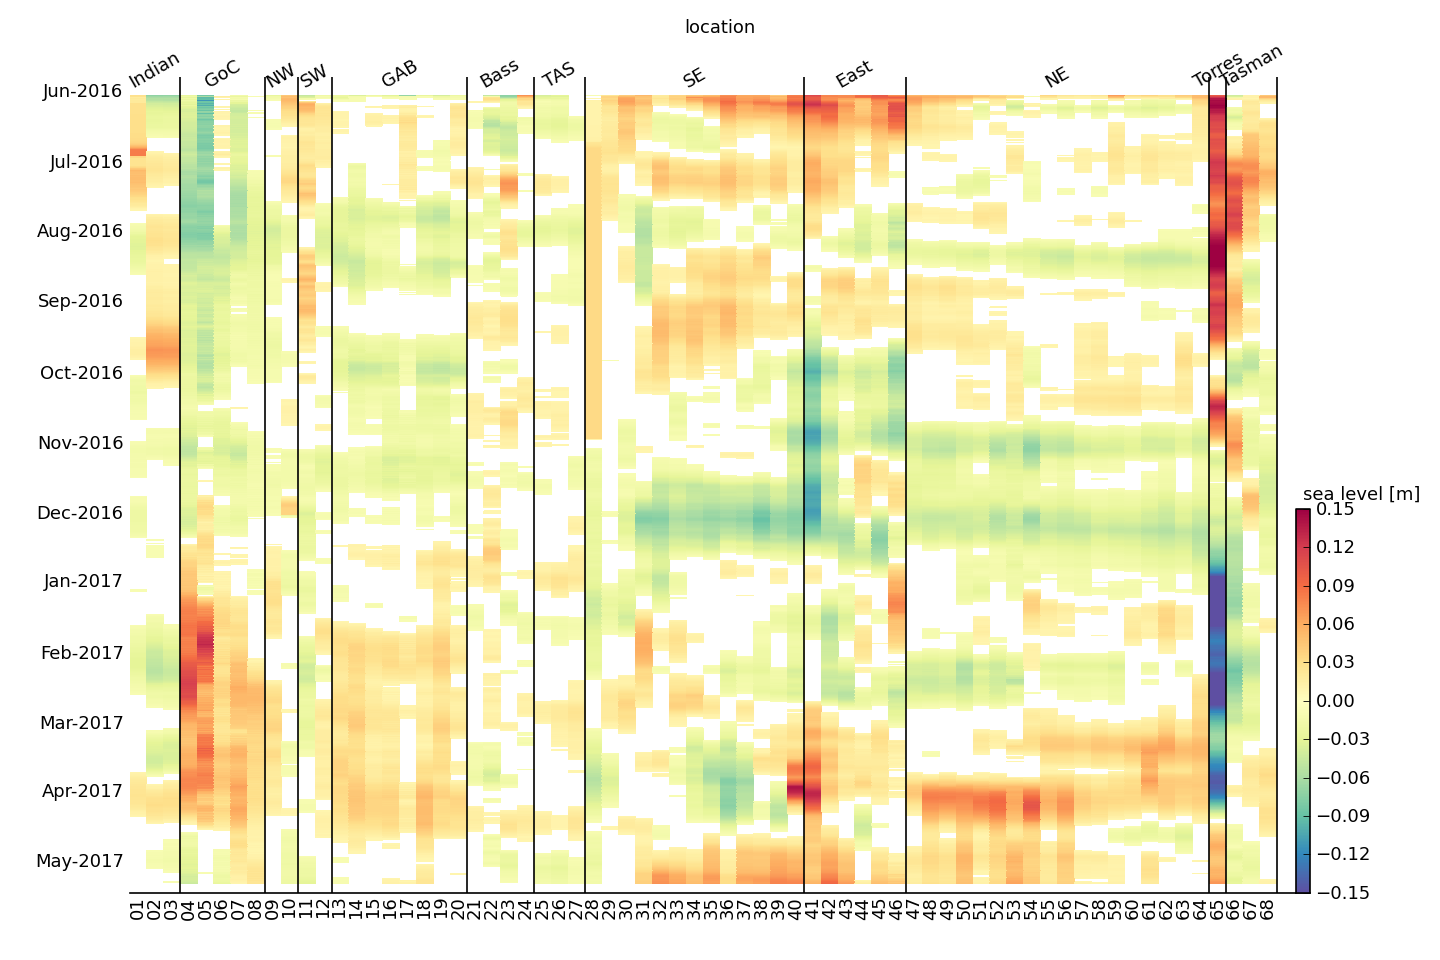
\includegraphics[width=1.0\textwidth]{plots/aggSL_bias_breakdown_plot_2.png}
\caption{Temporal signal from bias correction histories after subtraction of respective mean offsets.  Absolute values less than 0.01 m are shown as white.  A degree of coherence is apparent between adjacent sites within the regional groupings-shown on map in Figure \ref{fig:map_locations}. } 
\label{fig:bias_time}
\end{figure}  


%%%%%%%%%%%%%%%%%%%%%%%%%%%%%%%%%%%%%%%%%%
\section{Discussion}
\vspace{-6pt}
\subsection{Adequacy and Value}
The aggregation method offers generally improved sea level forecasts by drawing a pragmatic balance between the strengths of existing operational systems.
A common configuration for all sites was employed for robustness and to facilitate expansion to new locations.  
Although real-time observations are exploited when available, the simple bias correction scheme is relatively robust to data gaps and noise. 
The balance of contributions from component terms varies with timescale and location around the Australian coast.
Regional groupings are apparent in the skill characteristics of the forecasts.
By producing a quantity that can be directly compared to observations and reference tidal planes, forecasts can be presented intuitively along with recent real-time sea level and provide ongoing and immediate verification---as is Figure \ref{fig:fc_eg}.

The skill level and value offered by these forecasts sets a benchmark against which any new sea-level forecasting capabilities can be compared and contrasted.  

\subsection{Spatial Interpolation}
The characteristics demonstrated by the bias correction scheme indicate that meaningful forecasts may be produced at intermediate sites at which real-time observations are not available.
The patterns of regional coherence indicate that spatial interpolation of bias correction values may be worthy of further investigation.
Figure \ref{fig:bias_time} indicates that spatial interpolation within regions `GAB' and `NE' is particularly promising.

Appropriate consideration of geography and other factors on validity will be required.
Strongly contrasting bias correction characteristics at Torres Strait (site 65) highlight the importance of not ignoring geography.

While the irregular spatial sampling across the domain is undesirable, there is real prospect to obtain access to many more tide gauges that are known to exist but not report real time data to the BoM.   
Such additional locations will facilitate future investigation of spatial interpolation approaches.    


\subsection{Extensions}
The aggregation concept presented is flexible.
And it is foreseeable that additional or alternative operational inputs could be incorporated. 
The potential to seamlessly include short-range higher resolution forecast information, while maintaining the 7-day outlook, is a logical extension given the aim of exploiting existing capabilities.
On the other hand, NWP forecasts currently cover out to 10-days lead time. The option of extending the length of ocean forecasts to match is worthy of consideration in light of this sea level evaluation (such as in Figure \ref{fig:rms}).

Uncertainty information can already be roughly indicated by means of presenting overlaid sequential forecasts as in Figure \ref{fig:fc_eg}.
Optimal treatment of the lagged ensemble and communicating error growth to users is an outstanding need.
Developments in ensemble NWP systems within the operational center are expected to provide additional sampling of uncertainty and enable further development of this important aspect of sea level forecasts.  

%   %=====================================
%   % References, variant A: internal bibliography
%   %=====================================
%   %\begin{thebibliography}{999}
%   \bibliographystyle{mdpi}
%   %\renewcommand\bibname{References}
%   %\bibliography{ref_minimal}
%   \begin{thebibliography}{999}
%   \providecommand{\natexlab}[1]{#1}
%   
%   \bibitem[Bell \em{et~al.}(2009)Bell, Lef{\`e}bvre, Le~Traon, Smith, and
%     Wilmer-Becker]{Bell:2009uv}
%   Bell, M.J.; Lef{\`e}bvre, M.; Le~Traon, P.Y.; Smith, N.; Wilmer-Becker, K.
%   \newblock {GODAE The Global Ocean Data Assimilation Experiment}.
%   \newblock {\em Oceanography} {\bf 2009}, {\em 22}, 14--21.
%   
%   \bibitem[Pugh and Woodworth(2014)]{Pugh:2014di}
%   Pugh, D.; Woodworth, P.
%   \newblock {\em Sea-Level Science: Understanding Tides, Surges, Tsunamis
%     and Mean Sea-Level Changes}; Cambridge University Press: Cambridge, UK, 2014.
%   
%   \bibitem[Box(1979)]{Box:1979wz}
%   Box, G.
%   \newblock {Robustness in the strategy of scientific model building}.
%   \newblock {\em Robust. Stat.} {\bf 1979}, doi:10.1016/b978-0-12-438150-6.50018-2.
%   
%   \bibitem[Melet \em{et~al.}(2016)Melet, Almar, and
%     Meyssignac]{Anonymous:jdDiSHB0}
%   Melet, A.; Almar, R.; Meyssignac, B.
%   \newblock {What dominates sea level at the coast: A case study for the Gulf of
%     Guinea}.
%   \newblock {\em Ocean Dyn.} {\bf 2016}, \emph{66}, 623--636.
%   
%   \bibitem[Haigh \em{et~al.}(2013{\natexlab{a}})Haigh, Wijeratne, MacPherson,
%     Pattiaratchi, Mason, Crompton, and George]{Haigh:2013bna}
%   Haigh, I.D.; Wijeratne, E.M.S.; MacPherson, L.R.; Pattiaratchi, C.B.; Mason,
%     M.S.; Crompton, R.P.; George,~S.
%   \newblock {Estimating present day extreme water level exceedance probabilities
%     around the coastline of Australia: Tides, extra-tropical storm surges and
%     mean sea level}.
%   \newblock {\em Clim. Dyn.} {\bf 2013}, \emph{42}, 121--138.
%   
%   \bibitem[Haigh \em{et~al.}(2013{\natexlab{b}})Haigh, MacPherson, Mason,
%     Wijeratne, Pattiaratchi, Crompton, and George]{Haigh:2013hea}
%   Haigh, I.D.; MacPherson, L.R.; Mason, M.S.; Wijeratne, E.M.S.; Pattiaratchi,
%     C.B.; Crompton, R.P.; George,~S.
%   \newblock {Estimating present day extreme water level exceedance probabilities
%     around the coastline of Australia: Tropical cyclone-induced storm surges}.
%   \newblock {\em Clim. Dyn.} {\bf 2013}, \emph{42}, 139--157.
%   
%   \bibitem[Woodham \em{et~al.}(2013)Woodham, Brassington, Robertson, and
%     Alves]{Woodham:2013cl}
%   Woodham, R.; Brassington, G.B.; Robertson, R.; Alves, O.
%   \newblock {Propagation characteristics of coastally trapped waves on the
%     Australian Continental Shelf}.
%   \newblock {\em J. Geophys. Res. Oceans} {\bf 2013},  \emph{118}, 4461--4473.
%   
%   \bibitem[Ridgway(2004)]{Ridgway:2004kb}
%   Ridgway, K.R.
%   \newblock {The 5500-km-long boundary flow off western and southern Australia}.
%   \newblock {\em J. Geophys. Res.} {\bf 2004}, doi:10.1029/2003jc001921.
%   
%   \bibitem[Church and Freeland(1986)]{Church:1986tl}
%   Church, J.A.; Freeland, H.
%   \newblock {Coastal-trapped waves on the east Australian continental shelf. I:
%     Propagation of modes}.
%   \newblock {\em J. Phys. Oceanogr.} {\bf 1986}, \emph{16}, 1929--1943.
%   
%   \bibitem[Allen and Greenslade(2009)]{Allen:2009tf}
%   Allen, S.C.R.; Greenslade, D.J.M.
%   \newblock {\em A Spectral Climatology of Australian and South-West Pacific Tide
%     Gauges}; CAWCR Technical Reports; Centre for Australian Weather and Climate Research: Melbourne, VIC, Australia,~2009.
%   
%   \bibitem[Cartwright(2000)]{Cartwright:2000tt}
%   Cartwright, D.E.
%   \newblock {\em {Tides}}; Cambridge University Press: Cambridge, UK, 2000.
%   
%   \bibitem[Petersen(2012)]{Petersen:2012kp}
%   Petersen, A.
%   \newblock {\em {Simulating Nature}}; Chapman and Hall/CRC: London, UK,  2012.
%   
%   \bibitem[Schiller and Brassington(2011)]{Schiller:2011di}
%   Schiller, A.; Brassington, G.B.
%   \newblock {\em {Operational Oceanography in the 21st Century}}; Springer
%     Science + Business Media: Berlin, Germany, 2011.
%   
%   \bibitem[Harper(2008)]{Harper:kb}
%   Harper, K.C.
%   \newblock {\em {Weather by the Numbers}}; The MIT Press:  Cambridge, MA, USA, 2008.
%   
%   \bibitem[Paramygin \em{et~al.}(2017)Paramygin, Sheng, and
%     Davis]{Paramygin:2017dx}
%   Paramygin, V.; Sheng, Y.; Davis, J.
%   \newblock {Towards the Development of an Operational Forecast System for the
%     Florida Coast}.
%   \newblock {\em J. Mar. Sci. Eng.} {\bf 2017}, \emph{5}, 8.
%   
%   \bibitem[Yang \em{et~al.}(2016)Yang, Richardson, Chen, Kelley, Myers, Aikman,
%     Peng, and Zhang]{Yang:2016ep}
%   Yang, Z.; Richardson, P.; Chen, Y.; Kelley, J.; Myers, E.; Aikman, F.; Peng,
%     M.; Zhang, A.
%   \newblock {Model Development and Hindcast Simulations of NOAA{\textquoteright}s
%     Gulf of Maine Operational Forecast System}.
%   \newblock {\em J. Mar. Sci. Eng.} {\bf 2016}, \emph{4},~77.
%   
%   \bibitem[Wei \em{et~al.}(2014)Wei, Zhang, Yang, Chen, Kelley, Aikman, and
%     Cao]{Wei:2014ex}
%   Wei, E.; Zhang, A.; Yang, Z.; Chen, Y.; Kelley, J.; Aikman, F.; Cao, D.
%   \newblock {NOAA{\textquoteright}s Nested Northern Gulf of Mexico Operational
%     Forecast Systems Development}.
%   \newblock {\em J. Mar. Sci. Eng.} {\bf 2014}, \emph{2}, 1--17.
%   
%   \bibitem[Peng \em{et~al.}(2014)Peng, {Richard Jr}, Zhang, and {Frank
%     III}]{Peng:2014kq}
%   Peng, M.; {Schmalz, R.A., Jr.}; Zhang, A.; {Aikman, F., III}.
%   \newblock {Towards the Development of the National Ocean Service San Francisco
%     Bay Operational Forecast System}.
%   \newblock {\em J. Mar. Sci. Eng.} {\bf 2014}, \emph{2}, 247--286;
%   
%   \bibitem[Hendershott(1981)]{Hendershott:1981ub}
%   Hendershott, M.
%   \newblock {Long waves and ocean tides}. In {\em Evolution of Physical
%     Oceanography}; The MIT Press:  Cambridge, MA, USA, 1981.
%   
%   \bibitem[Foreman \em{et~al.}(2009)Foreman, Cherniawsky, and
%     Ballantyne]{Foreman:2009bg}
%   Foreman, M.G.G.; Cherniawsky, J.Y.; Ballantyne, V.
%   \newblock {Versatile Harmonic Tidal Analysis: Improvements and Applications}.
%   \newblock {\em J. Atmos. Ocean. Technol.} {\bf 2009}, doi:10.1175/2008JTECHO615.1.
%   
%   \bibitem[Groves and Reynolds(1975)]{Groves:1975ky}
%   Groves, G.W.; Reynolds, R.W.
%   \newblock {An Orthogonalized Convolution Method of Tide Prediction}.
%   \newblock {\em J. Geophys. Res.} {\bf 1975}, \emph{80}, 4131--4138. 
%   
%   \bibitem[Leffler and Jay(2009)]{LEFFLER:2009ej}
%   Leffler, K.; Jay, D.
%   \newblock {Enhancing tidal harmonic analysis: Robust (hybrid L1/L2L1/L2)
%     solutions}.
%   \newblock {\em Cont.~Shelf~Res.} {\bf 2009}, \emph{29}, 78--88.
%   
%   \bibitem[Smith \em{et~al.}(1997)Smith, Ambrosius, Wakker, Woodworth, and
%     Vassie]{Smith:1997ut}
%   Smith, A.; Ambrosius, B.; Wakker, K.F.; Woodworth, P.L.; Vassie, J.M.
%   \newblock {Comparison between the harmonic and response methods of tidal
%     analysis using TOPEX/POSEIDON altimetry}.
%   \newblock {\em J. Geod.} {\bf 1997},  \emph{71},  695--703.
%   
%   \bibitem[Mapping(2014)]{Mapping:2014wu}
%   Mapping, I.C.o.S.
%   \newblock {\em Australian Tides Manual};
%   \newblock {Technical Report; Permanent Committee on Tides and Mean Sea Level: Wollongong, Australia, 2014.}
%   %please confirm this accuracy ... details from here http://www.icsm.gov.au/tides/
%   
%   \bibitem[Parker(2007)]{Parker:2007wq}
%   Parker, B.B.
%   \newblock {\em Tidal Analysis and Prediction};
%   \newblock {Technical Report; National Oceanic and Atmospheric Administration - Center for Operational Oceanographic Products and Services: Silver Spring, Maryland, USA, 2007.}
%   
%   \bibitem[Ray and Egbert(2004)]{Ray:2004ts}
%   Ray, R.; Egbert, G.D.
%   \newblock {The Global S1 Tide}.
%   \newblock {\em J. Phys. Oceanogr.} {\bf 2004}, \emph{34}, 1922.
%   
%   \bibitem[Horsburgh \em{et~al.}(2008)Horsburgh, Williams, Flowerdew, and
%     Mylne]{Horsburgh:2008gw}
%   Horsburgh, K.J.; Williams, J.A.; Flowerdew, J.; Mylne, K.
%   \newblock {Aspects of operational forecast model skill during an extreme storm
%     surge event}.
%   \newblock {\em J. Flood Risk Manag.} {\bf 2008}, \emph{1}, 213--221.
%   
%   \bibitem[Egbert and Bennett(1996)]{Egbert:1996vr}
%   Egbert, G.D.; Bennett, A.F.
%   \newblock {Data assimilation methods for ocean tides}. \emph{Elsevier Oceanogr. Ser.} \textbf{1996}, doi:10.1016/s0422-9894(96)80009-2.
%   
%   \bibitem[Greenslade and Warne(2012)]{Greenslade:2012um}
%   Greenslade, D.J.M.; Warne, J.O.
%   \newblock {Assessment of the Effectiveness of a Sea-Level Observing Network for
%     Tsunami Warning}.
%   \newblock {\em J. Waterw. Port Coast. Ocean Eng.} {\bf
%     2012},  \emph{138}, 246--255.
%   
%   \bibitem[Horsburgh and De~Vries(2011)]{Horsburgh:2011th}
%   Horsburgh, K.; De~Vries, H.
%   \newblock {\em Guide to Storm Surge Forecasting};
%   \newblock Technical Report; World Meteorological Organization: Geneva, Switzerland, 2011.
%   %please provide the Publisher: City, Country before the year.
%   
%   \bibitem[Mourre \em{et~al.}(2006)Mourre, Crosnier, and Provost]{Mourre:2006hz}
%   Mourre, B.; Crosnier, L.; Provost, C.L.
%   \newblock {Real-time sea-level gauge observations and operational
%     oceanography}.
%   \newblock {\em Philos. Trans. R. Soc. A} {\bf 2006}, \emph{364}, 867--884.
%   
%   \bibitem[Taylor \em{et~al.}(2010)Taylor, Brassington, and Nader]{Taylor:2010ud}
%   Taylor, A.J.; Brassington, G.B.; Nader, J.
%   \newblock {\em Assessment of BLUElink OceanMAPSv1.0b Against Coastal Tide Gauges};
%   \newblock Technical Report; Centre for Australian Weather and Climate Research: Melbourne, VIC, Australia, 2010.
%   
%   \bibitem[Tilburg and Garvine(2004)]{Tilburg:2004cg}
%   Tilburg, C.E.; Garvine, R.W.
%   \newblock {A Simple Model for Coastal Sea Level Prediction}.
%   \newblock {\em Weather Forecast.} {\bf 2004}, doi:10.1175/1520-0434(2004)019<0511:ASMFCS>2.0.CO;2.
%   
%   \bibitem[Taylor \em{et~al.}(2011)Taylor, Smith, Wang, Robinson, and
%     Brassington]{Taylor:2011ud}
%   Taylor, A.J.; Smith, A.; Wang, W.; Robinson, J.; Brassington, G.B.
%   \newblock {Ocean meets river: Connecting Bureau of Meteorology ocean forecasts
%     and river height predictions for improved flood warnings}.
%   \newblock  In Proceedings of the 19th International Congress on Modelling and Simulation, Perth,
%     Australia, 12--16 December 2011. 
%    %^ http://mssanzorgau/modsim2011,
%     
%   
%   \bibitem[Brassington \em{et~al.}(2007)Brassington, Pugh, Spillman, Schulz,
%     Beggs, Schiller, and Oke]{Brassington:2007ut}
%   Brassington, G.B.; Pugh, T.; Spillman, C.; Schulz, E.; Beggs, H.; Schiller, A.;
%     Oke, P.R.
%   \newblock {BLUElink> Development of Operational Oceanography and Servicing in
%     Australia}.
%   \newblock {\em J. Res. Pract.  Inf. Technol.} {\bf
%     2007}, \emph{39}, 151--164.
%   
%   \bibitem[{Bureau of Meterology}(2007)]{NMOC:2007wq}
%   {Bureau of Meterology}.
%   \newblock {\emph{Implementation of OceanMAPS (BLUElink> Ocean Forecast
%     System)}};
%   \newblock Technical Report; Bureau of Meteorology: Melbourne, VIC, Australia, 2007.
%   
%   \bibitem[{Bureau of Meterology}(2011)]{BureauofMeterology:2011ta}
%   {Bureau of Meterology}.
%   \newblock {\em Operational Upgrades to OceanMAPS (BLUElink> Ocean Forecast
%     System)};
%   \newblock Technical Report; Bureau of Meteorology: Melbourne, VIC, Australia, 2011.
%   
%   \bibitem[Brassington \em{et~al.}(2012)Brassington, Freeman, Huang, Pugh, Oke,
%     Sandery, Taylor, Andreu-Burillo, Schiller, Griffin, Fiedler, Mansbridge,
%     Beggs, and Spillman]{Brassington:2012wm}
%   Brassington, G.B.; Freeman, J.; Huang, X.; Pugh, T.; Oke, P.; Sandery, P.A.;
%     Taylor, A.J.; Andreu-Burillo,~I.; Schiller,~A.; Griffin,~D.; et al. 
%   \newblock {\em Ocean Model, Analysis and Prediction System: Version 2};
%   \newblock Technical Report;  Centre for Australian Weather and Climate Research: Melbourne, VIC, Australia, 2012.
%   
%   \bibitem[Griffies \em{et~al.}(2008)Griffies, Harrison, Pacanowski and Rosati]{Griffies:2008vh}
%   Griffies, S.M.; Harrison, M.; Pacanowski, R.
%   \newblock {\em A Technical Guide to MOM4};
%   \newblock Technical Report; NOAA/Geophysical Fluid Dynamics Laboratory: Princeton NJ, USA, 2008.
%   
%   \bibitem[Oke \em{et~al.}(2008)Oke, Brassington, and Griffin]{Oke:2008wr}
%   Oke, P.; Brassington, G.B.; Griffin, D.
%   \newblock {The Bluelink ocean data assimilation system (BODAS)}.
%   \newblock {\em Ocean Model.} {\bf 2008},  \emph{21}, 46--70.
%   
%   \bibitem[{Bureau of Meterology}(2016)]{BureauofMeterology:C8IaJ2Qq}
%   {Bureau of Meterology}.
%   \newblock {\em APS2 Upgrade to the ACCESS-G Numerical Weather Prediction System};
%   \newblock Technical Report;  Bureau of Meteorology: Melbourne, VIC, Australia, 2016.
%   
%   \bibitem[Brassington(2013)]{GaryBBrassington:2013jw}
%   Brassington, G.B.
%   \newblock {Multicycle ensemble forecasting of sea surface temperature}.
%   \newblock {\em Geophys. Res. Lett.} {\bf 2013}, \emph{40},~6191–6195.
%   
%   \bibitem[Mathers and Woodworth(2004)]{Mathers:2004bk}
%   Mathers, E.L.; Woodworth, P.L.
%   \newblock {A study of departures from the inverse-barometer response of sea
%     level to air-pressure forcing at a period of 5 days}.
%   \newblock {\em Q. J. R. Meteorol. Soc.} {\bf
%     2004}, \emph{130}, 725–738.
%   
%   \bibitem[Murphy(1993)]{Murphy:1993dh}
%   Murphy, A.H.
%   \newblock {What Is a Good Forecast? An Essay on the Nature of Goodness in
%     Weather Forecasting}.
%   \newblock {\em Weather Forecast.} {\bf 1993}, \emph{8}, 281–293.
%   
%   \bibitem[Taylor(2000)]{Taylor:2000wp}
%   Taylor, K.
%   \newblock {\em Summarizing Multiple Aspects of Model Performance in a Single
%     Diagram};
%   \newblock Technical Report; Program For Climate Model Diagnosis And
%     Intercomparison University Of California, Lawrence Livermore National
%     Laboratory: Livermore, CA, USA, 2000.
%   
%   \bibitem[Slobbe \em{et~al.}(2013)Slobbe, Verlaan, Klees, and
%     Gerritsen]{Slobbe:wk}
%   Slobbe, D.C.; Verlaan, M.; Klees, R.; Gerritsen, H.
%   \newblock {Obtaining instantaneous water levels relative to a geoid with a 2D
%     storm surge model}.
%   \newblock {\em Cont. Shelf Res.} {\bf 2013}, \emph{52}, 172--189.
%   
%   \bibitem[Oke \em{et~al.}(2013)Oke, Griffin, and Schiller]{Oke:2013fm}
%   Oke, P.; Griffin, D.; Schiller, A.
%   \newblock {Evaluation of a near-global eddy-resolving ocean model}.
%   \newblock {\em Geosci. Model Dev.} {\bf 2013}, \emph{6}, 591--615.
%   
%   \end{thebibliography}


		\chapter{Viewing and evaluating forecasts on a coastal waveguide}
\label{chp:waveguide}

\begin{quote}
{\small
An approach to reduce forecast data to coastal waveguide coordinates is described and demonstrated; informed by the literature on coastally trapped waves (CTW).  All discussion is limited to the Australian mainland but the approach is generally relevant to regions where CTWs influence sea level; including the Americas and Africa. The approach does not produce new forecasts, but aims to focus forecaster attention on aspects of sea level forecasts prominent on the long Australian coast.  The approach also explicitly addresses spatial issues associated with measuring coastal paths. 
Coastal paths are scale-dependent and forecast models discretise the coastal boundary differently. 
A well defined coastal path is required for the quantitative application of CTW concepts such as propagation distance and offshore direction.
The relevance of coastally trapped signals and remote forcing is documented in the oceanographic literature, but is effectively unknown to the general public and rarely mentioned in press reports of sea level events such as nuisance flooding.
Routine presentation of forecast guidance in waveguide coordinates could contribute to the transfer of oceanographic research understanding into forecast narratives.
In addition, the approach can facilitate quantitative forecast evaluations that target CTW properties.
Two ocean forecast systems are contrasted in this framework for the Australian mainland.
One year of daily forecasts are compared, with indications that model baroclinicity is of practical relevance.  
}
\end{quote} 

%--------------------------------------------------------------------------
% introduction
%--------------------------------------------------------------------------
\section{Sea level anomalies and forecast narratives}

Many activities are organised around expectations of coastal water levels over the next few days, including mitigation of  nuisance coastal flooding \citep{Sweet:2014ss, Hague:2019ha}

Still water levels \citep{Pugh:2014di} at the coast are not just a matter of tidal patterns and local storms, but can also be influenced by remote forcing via coastally trapped wave (CTW) mechanisms.
Whilst CTWs have received much academic attention (Section \ref{sec:ctw_background}), it seems the application of the CTW perspective to the evaluation of model guidance and the creation of forecast narratives is routinely absent in the Australian setting. 
This leaves both forecasters and the public with a common assumption that coastal sea level anomalies are driven solely by local weather. Such assumptions may arguably be reinforced by the the manner in which forecasts and evaluation metrics are routinely presented.

Very high impact short scale extreme such as tropical cyclones \citep{McInnes:2016km} are obviously important to coastal decisions but are not the target of this discussion. 


Coastal sea level anomalies are in practice almost always interpreted with reference to conventional tide tables \citep{PCTMSL:2018}.
Whilst sophisticated sea level decision support systems do exist for some customers \citep{James:2017gj}, in general circumstances the coastal community consult tide tables in light of recently observed anomalies and anomaly trend expectations.
Expectations of how anomalies (or `residuals') may change over the next few days can be based on recent observations, heuristics and numerical forecast guidance \citep{Taylor:2017co, Horsburgh:2011th}.   Numerical forecasts are the focus of this discussion.
Numerical forecasts of sea level anomaly fields are commonly viewed as topographic maps like Figure \ref{fig:oldcharts}.
%----------------------------
% map guidance
\begin{figure}[H]\centering
    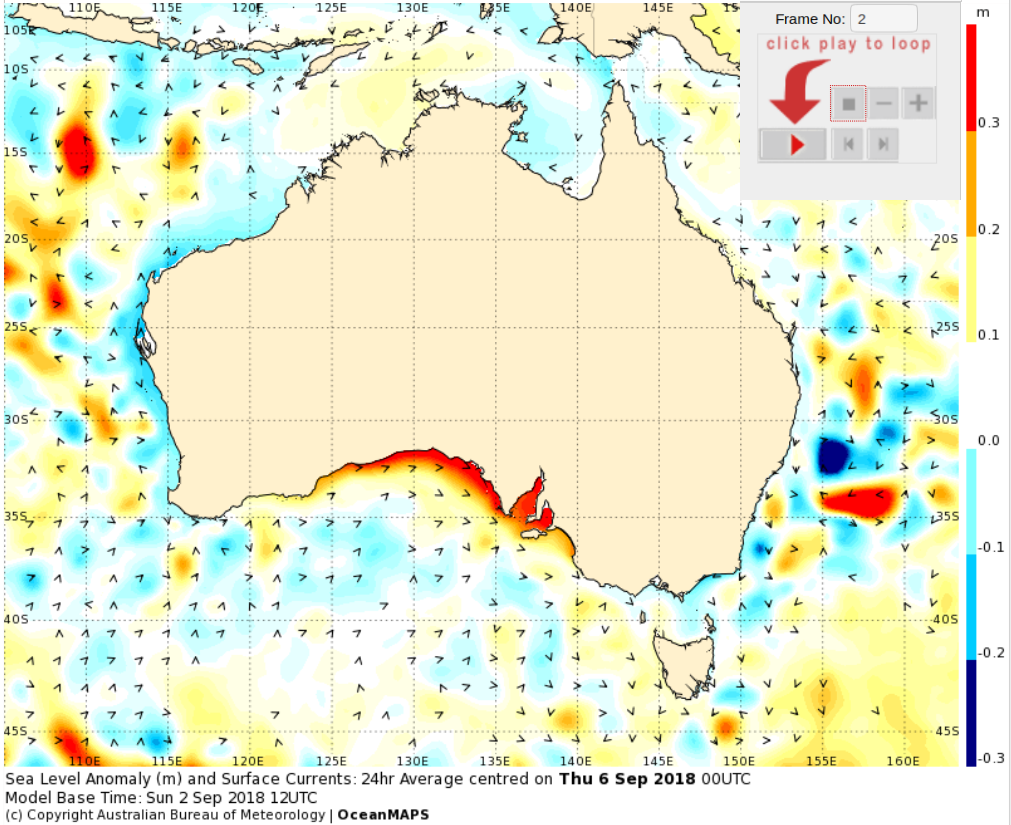
\includegraphics[width=\figwidthBig]{figures/maps/omaps_chart_anim_eg.png}
    \caption[OceanMAPS SLA chart from the Bureau's public website]{ OceanMAPS SLA chart from the Bureau's public website;
              whilst moving patterns are often noticeable when animated, these displays do not inherently focus on coastal aspects of the forecast.  \protect\citep{urlBOM_SLA:2018} }
    \label{fig:oldcharts}
\end{figure}  
%----------------------------
Coastal propagation of sea level features can be noticed on animated versions of such maps if the spatial scope is sufficiently large.
But with a wide scope the coastal signal is often visually swamped by the diverse phenomena thus included; such as the eddies shown off the east coast of Australia.
In contrast to the `map' view, consider the propagation-focused phase-space guidance available to tropical weather forecasters \citep{doi:10.1175/1520-0493(2004)132<1917:AARMMI>2.0.CO;2} that reduces the many dimensions of a numerical forecast to the propagation of particular patterns around the equatorial wave guide.

Regardless of the forecast guidance source, narrative attribution can be a factor that influences decisions.  
If residents are told that ``...westerly winds push tides from the bay..'' \citep{urlMW:2018}, then they may be perplexed to find their sea gate closed on a windless day.  Public messaging about local strong winds and low pressure are common and useful enough:
``...storm surge is caused when a low atmospheric pressure meteorological system and \emph{strong onshore winds} force sea levels to rise above normal levels...''
\citep{urlBris:2018}.  But the role of \emph{remote} winds, wind orientation, persistent and propagating sea level signals seems to be effectively ignored from such descriptions.  


Essentially, we perceive a gap between research understanding and daily forecast narratives.
Routine availability of waveguide views into numerical forecast data may contribute to the transfer of academic understanding to a wider audience and ultimately to improved communications regarding coastal sea level.
Waveguide-based methods to inter-compare heterogeneous forecast data may also facilitate the connection between aspects of the research literature to operational verification and systems development.

We demonstrate one approach for projecting operational ocean forecast data into waveguide coordinates.  Whilst our scope is restricted to the Australian mainland, the concepts may also be relevant to other regions.


%--------------------------------------------------------------------------
% CTW perspective
%--------------------------------------------------------------------------
\section{Coastal Waveguide Perspective}
\label{sec:ctw_background}

\subsection{Oceanographic literature}
The oceanographic literature addressing coastally trapped waves (CTW) is extensive and has prominently featured the Australian mainland. 
The literature has established a common spatial paradigm \citep{Brink:1991dl}  with directions relative to the coast as illustrated in Figure \ref{fig:ctw_typical}. In this context the nomenclature of longshore,alongshore and alongshelf are synonomous. This CTW `natural coordinate' system \citep{gill1982atmosphere} arises from an interest in propagation along a long coastal waveguide. The coordinate schematic indicates an ideal of uniformity long shore and a cross shelf profile that is either flat or deepening monotonically away from a coastal boundary.  
This situation allows for the hybrid of propagation mechanisms involving gravity and potential vorticity, requiring topographic slope, and Rossby adjustment against a coastal boundary.   

%----------------------------
% coord system
\begin{figure}[H]\centering
    \noindent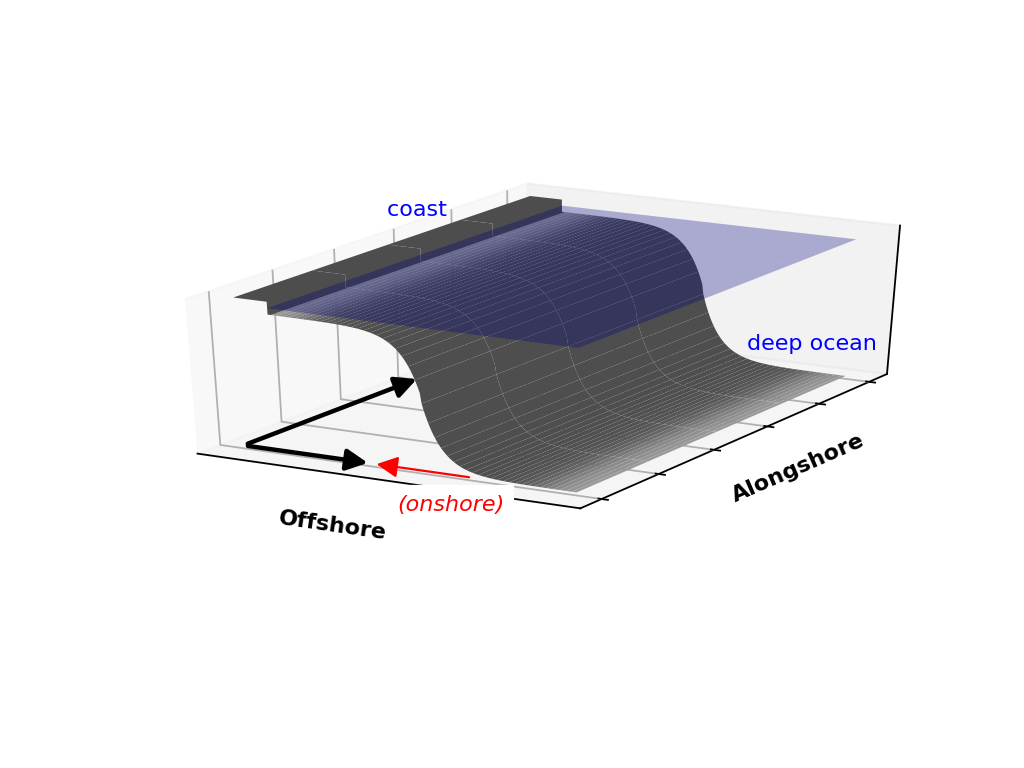
\includegraphics[width=\figwidthFull]{figures/diagrams/ctw_coords.png}
    \caption[Coastally trapped wave idealised coordinates]
             {Coastally trapped wave idealised coordinates and bathymetry profile. 
              Uniform and large scale in the longshore direction, with a coastal boundary and bathymetry either flat or monotonically increasing offshore. In the southern hemisphere CTWs propagate with the coast on the left. The term CTW covers the range of Kelvin and continental shelf wave mechanisms.  Following \protect\citep{Dale:2001dn}. }
    \label{fig:ctw_typical}
\end{figure}  
%----------------------------
CTW dynamics are generally associated with
sub-inertial frequencies, 
along shelf scales of motion much greater than cross shelf,  
along shelf propagation characteristics
and cross shelf mode decomposition.
Targeted campaigns have demonstrated the relevance of this theory to explaining non-tidal oceanographic observations \citep{Church:1986tl,Merrifield:1992ef,Ding:2012im}.
Coastal trapping also plays an important role in the astronomical tide literature \citep{Anonymous:cyAnLqia}.
The limits of CTW theory have been explored in the literature and these limits are relevant to application at routine weather forecast timescales.
For instance; 
\begin{itemize}
\item energy scattering and leakage \citep{Middleton:1991dq, Merrifield:1994et, Yankovsky:2017en}
\item near inertial and super-inertial frequencies \citep{Dale:2001dn, Dale:1996go} 
\item small scale geometrical irregularities \citep{Wilkin:1990iw,doi:10.1175/JPO-D-18-0106.1}
\item curvature of along shelf geometry \citep{Grimshaw:1977vu}
\item sensitivity to model choice \citep{Sanson:2012bu}
\item propagating atmospheric features at near resonant speeds \citep{McInnes:2003vl};
\end{itemize}

%-----------------------------------------------
\subsection{How long is the coast and where is it?}
\label{sec:ctw_waveguide}

Applying a CTW perspective to real geography raises the deceptively simple questions of how to measure the length of a propagation path and how to specify along and offshore directions.
Such questions are not problematic for the equatorial waveguide.
But for measuring a waveguide associated with land/sea boundary  raises the well-known `coastline paradox'; by which the length of a statistically fractal feature depends on the measuring scale \citep{Mandelbrot:1967hr} (introduced by L.F.Richardson in another context \citep{Vulpiani2014}).
The literature on CTWs, which inherently involves coastlines, has not directly addressed the statistically fractal character in the attribution of a propagation distance, wind direction or the separation between tide gauges.
Some non-oceanographic literature has however drawn connections in the opposite direction; between the complexity of the Australian coast and marine processes \citep{PORTERSMITH20121}.

In addition to the non-trivial task of measuring a coast, each discretised model carries its own representation of the coastal interface, often via a binary land/sea mask.
The defacto location of a numerical coast described by a mask can differ noticeably between models even if based on the same foundational bathymetry.
Such differences are especially significant with comparing models configured at different spatial resolutions. 



This situation motivates the application of an algorithmic method to realise a set of model-independent `waveguide' coordinates.
Fundamentally, such an algorithm is a means of defining a coastal path and associated local horizontal directions given a well-defined length scale.
For the present demonstration, a version of the traditional `divider walk' \citep{XU1993245} algorithm provided a tractable approach to develop a path using the Geospatial Data Abstraction library GDAL \citep{gdal}. 
The path used was based on a relatively high resolution ($\sim$250m) coastline dataset independent from the forecast models themselves.
Figure \ref{fig:mandelbrot_lengths} demonstrates the dependence of waveguide length on divider scale by multiple applications of the algorithm.  The dependence results in an estimate of an effective fractal dimension of $\sim$1.08, comparable to those summarised in \cite{MA2016}.
%----------------------------
% coastline length 
\begin{figure}[H]\centering
    \noindent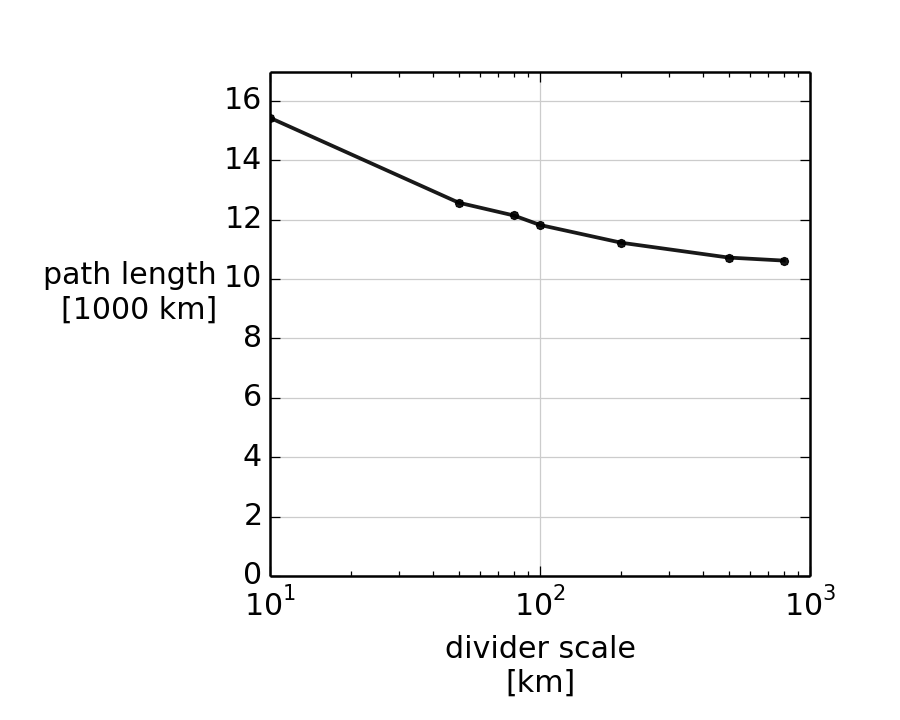
\includegraphics[width=\myfigwidthHalf]{figures/plots/mandelbrot_lengths.png}
    \caption[Waveguide length dependence on scale]{Total lengths of waveguide paths as a function of fixed divider scales, from which an effective fractal dimension of $\sim$1.08 is derived.  
All walk the same anti-cyclonic direction around the coast from an arbitrary start point near Darwin to and end point at Cape York. 
The final divider length in each case is allowed to vary in order to ensure identical start and end points.}
    \label{fig:mandelbrot_lengths}
\end{figure}  
%----------------------------
We emphasise that the idea is to define a longshore length-scale in the realisation of the waveguide path, such that distances and directions have an explicit foundation.
The particular algorithm and scale are not asserted as being unique or optimal and others may present benefits (e.g. the rolling ball method of \citet{Hall:2002bo}).
For this implementation, the length-scale of each divider segment is set proportional to a local Rossby radius of deformation \citep[p.205]{gill1982atmosphere} which is well-defined for the Australian continental path shown.   
This radius depends only on latitude and a wave celerity, which we have configured to match the barotropic mode at a nominal depth of 20m.

This configuration is intended to roughly target the longshore scales associated with CTW generation, but alternative realisations are plainly possible.
The choice of scale primarily impacts the sample directions and derivation of wave speeds from model output - it has no impact whatsoever on the source model's representation of phenomena.
Decomposition of wind vectors into along and offshore directions is closely tied to the details of the path definition.
Sensitivity of the results to the details of path realisation are not explored in this study but will be pursued in future work.      


Figure \ref{fig:CTW_path} shows the waveguide path referenced in subsequent figures.
The shorter lines at each vertex indicate the local offshore direction used to decompose wind vectors and sample coastal cells.
Only the Australian mainland is included with arbitrary start and end points.
Signal expressions around Tasmania or any smaller islands are not addressed. 
%----------------------------
% map waveguide
\begin{figure}[H]\centering
    \noindent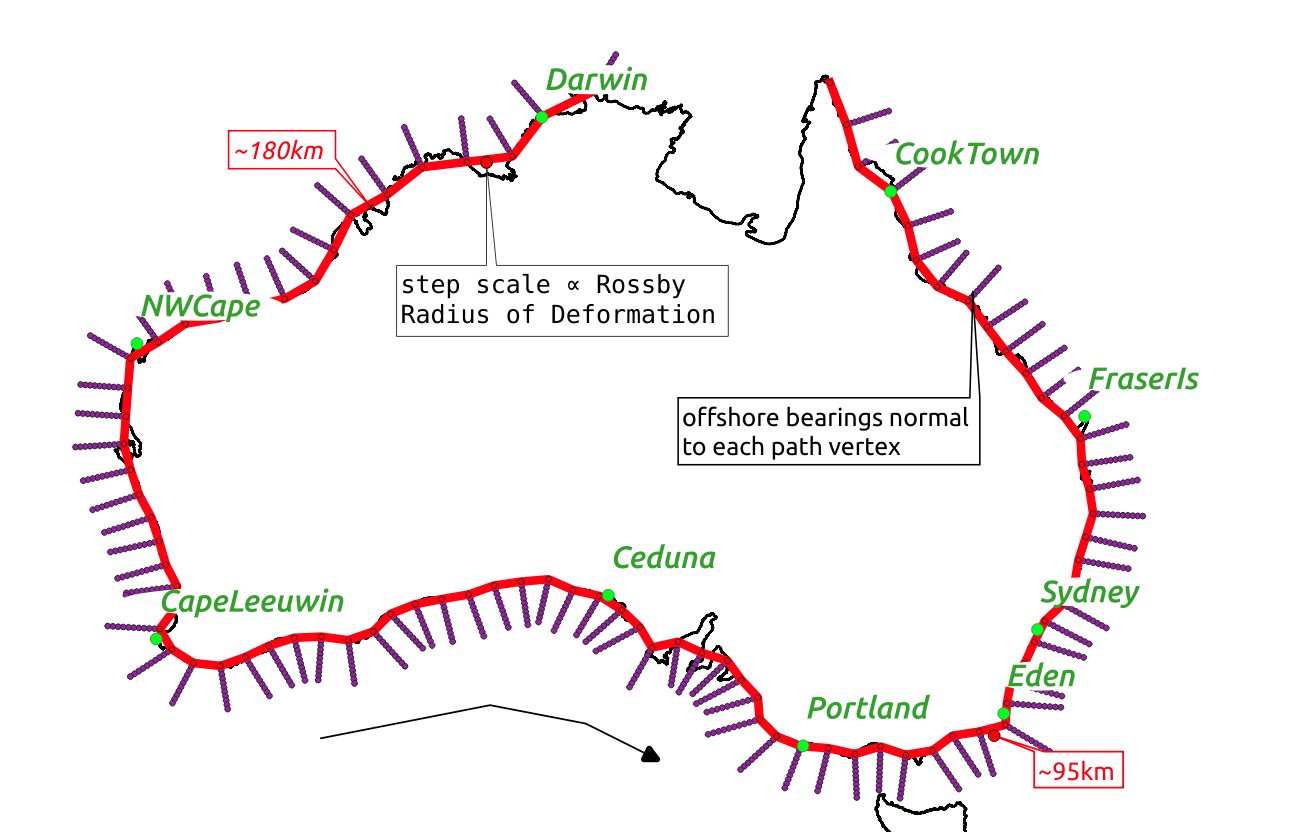
\includegraphics[width=\figwidthHalf]{figures/maps/map_overview.png}
    \caption[Coastal waveguide path around the Australian mainland used for this study.]
            {A coastal waveguide path around the Australian mainland with anticyclonic direction indicated (southern hemisphere).
             For this realisation, segment lengths $\protect\propto$ a Rossby Radius of Deformation measure. 
             Across-shore directions (short dark lines) are only locally orthogonal to the path but provide a means to assign a distance coordinate to model samples. 
             The start point is arbitrary and Tasmania is excluded.
             Locations are named to assist cross-referencing in subsequent figures.}
    \label{fig:CTW_path}
\end{figure}  
%----------------------------

%-------------------------------------------------
\subsection{ Projection onto the waveguide path }

The waveguide path is based on an independent high resolution coastline and choice of length scale.
Different data sources were projected onto this path using an algorithmic sampling method.
The sampling method aims to select only grid cells represented as coastal in each model, and to associate locations with the waveguide via orthogonal projection. 
This is effectively a restricted type of `nearest neighbour' sampling with no interpolation between grid points.

For each cross-shore profile line in Figure \ref{fig:CTW_path}, the algorithm essentially looks for the best matching coastal cell by starting out to sea and stepping inwards until the last `wet' cell is found.
Each sample is associated with longshore distance coordinate of the corresponding waveguide vertex.

For tide gauge observations, the inverse process was applied as a geometric projection to assign a waveguide coordinate. 
The projection mapped each tide gauge location to the single closest point on the waveguide following a bearing perpendicular to the matched line segment. 
An arbitrary limit of 50km was applied to limit the spatial extent of the automated projection - which otherwise could match distant island locations to the coastal path. 

To facilitate additional post-processing of the waveguide sampled datasets a two stage linear interpolation process was applied to reduce the data further to a common regular time and space grid for differencing and correlation operations.  

%--------------------------------------------------------------------------
% data
%--------------------------------------------------------------------------
\section{Data Sources from the Operational Centre}

This study originates from the application of a CTW perspective within an operational setting.
Key details of the operational data sources used are outlined below.
Data availability has limited our comparison to the 1-year period from 10-April 2018 to 10-April 2019.

%-----------------------
\subsection{Surface winds and pressure from NWP: ACCESS-G }
\label{sec:access}
Atmospheric forecast inputs were taken from the global numerical weather prediction (NWP) system ACCESS-G \citep{BureauofMeterology:C8IaJ2Qq}.
It is not coupled with any ocean model and employs an observational SST analysis, fixed over each forecast, as a lower boundary condition.
These flux fields are generated on a N512 Gaussian grid with an indicative spatial resolution of $\sim$25km. 

%-----------------------
\subsection{OceanMAPS: Data Assimilating Global Primitive Equation Forecasts }
\label{sec:oceanmaps}
7-day sea level anomaly (SLA) forecasts were taken from the near-global Ocean Model, Analysis and Prediction System (OceanMAPS).
OceanMAPS has now been in operational production for over 10 years across several version upgrades  
\citep{Brassington:2007ut,NMOC:2007wq,BureauofMeterology:2011ta,Brassington:2012wm}.
The dynamic ocean model component of OceanMAPS is based on the Modular Ocean Model (MOM version 4.1) \citep{Griffies:2008vh} configured with a 0.1x0.1 degree regular structured horizontal resolution, hydrostatic free surface, 51 z-levels with 5m top cell, 15m minimum column depth and a split-implicit scheme; where the barotropic calculation is performed at a finer time stepping. 
Atmospheric fluxes from ACCESS-G including surface stress are imposed directly.
Note that barometric pressure and gravitational tidal forces are intentionally \textit{not} applied.

Initial conditions for the ocean state are constrained using an ensemble optimal interpolation data assimilation scheme \citep{Oke:2008wr, sakov:2014}. 
Tide gauge observations are \textit{not} assimilated and are independent.   
Satellite altimeter observations of sea level are assimilated, but not inshore of the shelf break; nominally cut off at the 200m isobath. 
Background error covariances are non-gaussian and based on physical scales resolved by the model.

OceanMAPS produces a new ocean state forecast each day using a multi-cycle ensemble schedule \citep{GaryBBrassington:2013jw}.

Concatenated OceanMAPS data for the period are shown in Figure \ref{fig:hov_eg}. 
%----------------------------
% sla hovmuller
\begin{figure}[H]\centering
    \noindent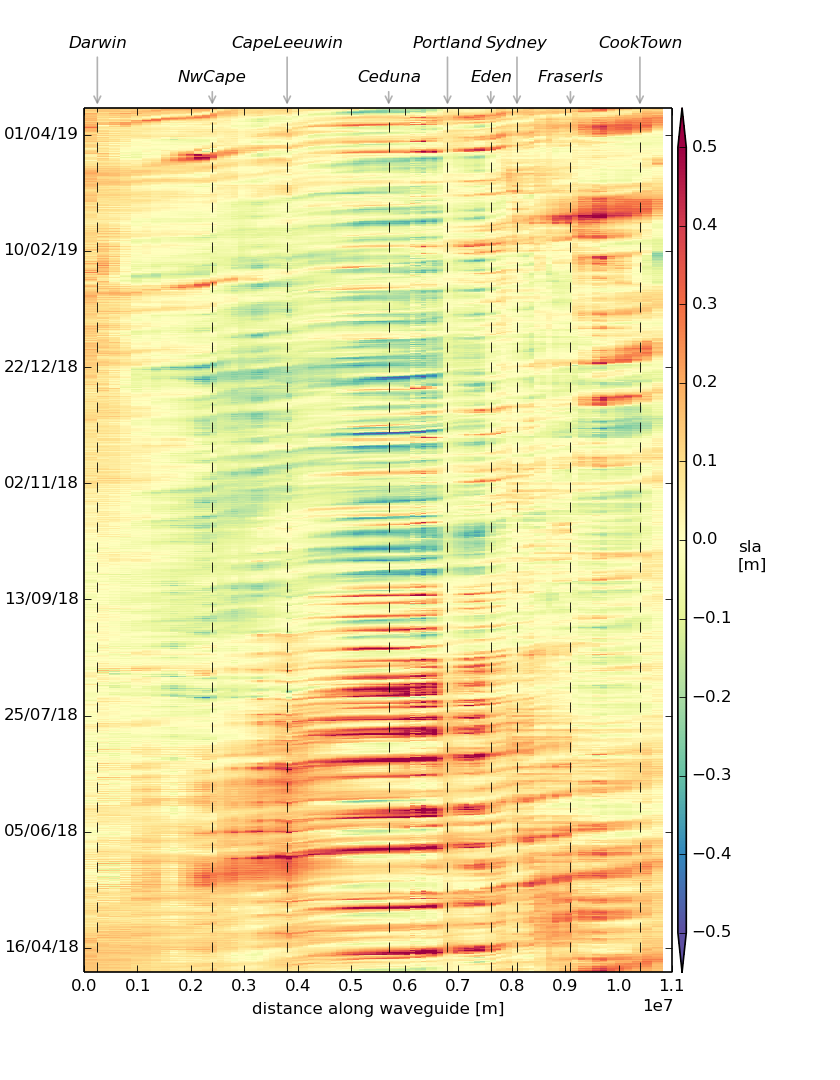
\includegraphics[width=\figwidthFull]{figures/plots/concat_sla_day0_full.png}
    \caption[Concatenated first day of OceanMAPS SLA forecasts] 
            {Concatenated first day of OceanMAPS SLA forecasts for the comparison period, 
             timeseries at each position centred by removal of sample mean. Note the distance units are meters and range to $\sim$11000km}
    \label{fig:hov_eg}
\end{figure} 
%----------------------------

%-----------------------
\subsection{Surge: Regional Shallow Water Depth Integrated  }
\label{sec:roms}
Three-day surge forecasts are taken from a national domain 2D configuration of ROMS \citep{Shchepetkin:2005eh} which has been brought into operational production more recently \citep{Allen:2018aa}.  
This operational system produces new forecasts on a 6-hourly warm start cycle with atmospheric forcing from the regional NWP forecasts (ACCESS-R).
No data assimilation is employed and the regional domain is \emph{not} nested in any larger model.
Whilst no baroclinic dynamics are included, the system offers relatively high spatial resolution of $\sim2km$ and alignment with weather forecasts from the more rapidly updated regional NWP system.


For the purposes of this study, a variant of the operational 2D ROMS forecast schedule was run using the identical NWP inputs to the 3D global model, namely ACCESS-G.   
Unlike the operational surge system, barometric pressure fields where \emph{not} applied to this variant to facilitate direct model inter comparison with OceanMAPS.
Henceforth this system will be referred to as `Surge'.
Whilst this is not strictly operational output, utilising the common NWP source facilitates more meaningful contrast of the ocean model types. 
Modifications beyond the exchange of source NWP were avoided and forecast length was kept at 72 hours.


%-----------------------
\subsection{ Adjusted Tide Gauge Observations }
In-situ coastal sea level observations were obtained from a heterogeneous set of real-time tide gauges. 
Many more tide gauges are known to exist within our spatial domain, but we have intentionally used only datastreams available in real-time to Bureau operations.
The resulting spatial sampling of the network is very irregular. 
Coverage along the east coast is most comprehensive.   
The fact that only a subset of these available tide gauges are co-located with barometer instruments influenced the choice to apply a NWP-based inverse barometer adjustment.
This local inverse barometer approximation approach is simplistic \citep{Mathers:2004bk} but pragmatic and formatted as follows:
$ \eta_{LIB} = \frac{ p_{NWP} - p_{ref} }{ \rho g } $
, where reference pressure is fixed at $p_{ref}=101325Pa$, and bulk sea water density is also kept fixed at $1027\frac{kg}{m^3}$. 
Several steps of processing were applied to obtain comparable adjusted residuals.
(1) temporal homogenisation to 1-hour averages (2) subtraction of standard harmonic tide signal (3) adjustment using local inverse barometer approximation based on NWP pressure field.

%--------------------------------------------------------------------------
% comparisons
%--------------------------------------------------------------------------
\section{Viewing operational data in CTW coordinates}

CTWs around the Australian mainland have been recently discussed in the context of general primitive equation ocean models by \citet{Woodham:2013cl} and \citet{Liao:2018jd}; and in the north west of Australia by \cite{Maxime:2019jc}.  The models discussed are closely related to the operational OceanMAPS system. 
In line with the previous literature, these papers address propagation speeds but not how distances between sample locations where measured.
We assert that propagation quantities are rendered more meaningful in this context when the propagation path is made explicit.
The explicit waveguide path approach described in Section \ref{sec:ctw_waveguide} facilitates the generation of new guidance to focus attention on coastal patterns and helps clarify the attribution of propagation quantities.  
Figure \ref{fig:hov_eg} shows a concatenation of the first 24-hours of each OceanMAPS forecast as a familiar `trough-and-ridge' plot \citep{hovmoller:1949}.
Select place names around the Australian mainland are indicated for reference.
Diagonal patterns sloping upward to the right are indicative of signal movement in an anti-cyclonic direction (counter clockwise for the Southern hemisphere).  Both positive and negative signals of this type are evident in many instances.
In contrast, essentially flat (i.e. not propagating) patterns that rise and fall with diurnal frequency are seen in the tropical sections of the domain.   


This projection approach is not limited to a single model or quantity; Figure \ref{fig:collate_g} illustrates an application to several forecast sources sharing a single base date.
A novel aspect of the application to surface winds (a vector quantity) is the decomposition into waveguide-based components - in which the directions are directly related to the length scale specified.
Surface winds are the primary driver of synoptic-scale sea level anomalies and the present inter-comparison is founded on identical atmospheric forcing source being applied to both models. As noted in Section \ref{sec:roms} the 2D surge forecasts are restricted to 3 days.
Broad correspondence of wind stress ($\tau$) and sea level patterns can be seen, especially along the southern shelves as described by \cite{McInnes:2003vl}.
In contrast a relatively regular diurnal pattern is notable in the tropical sections.
%----------------------------
% forecast collection of Hovmullers
\begin{figure}[H]\centering
    \noindent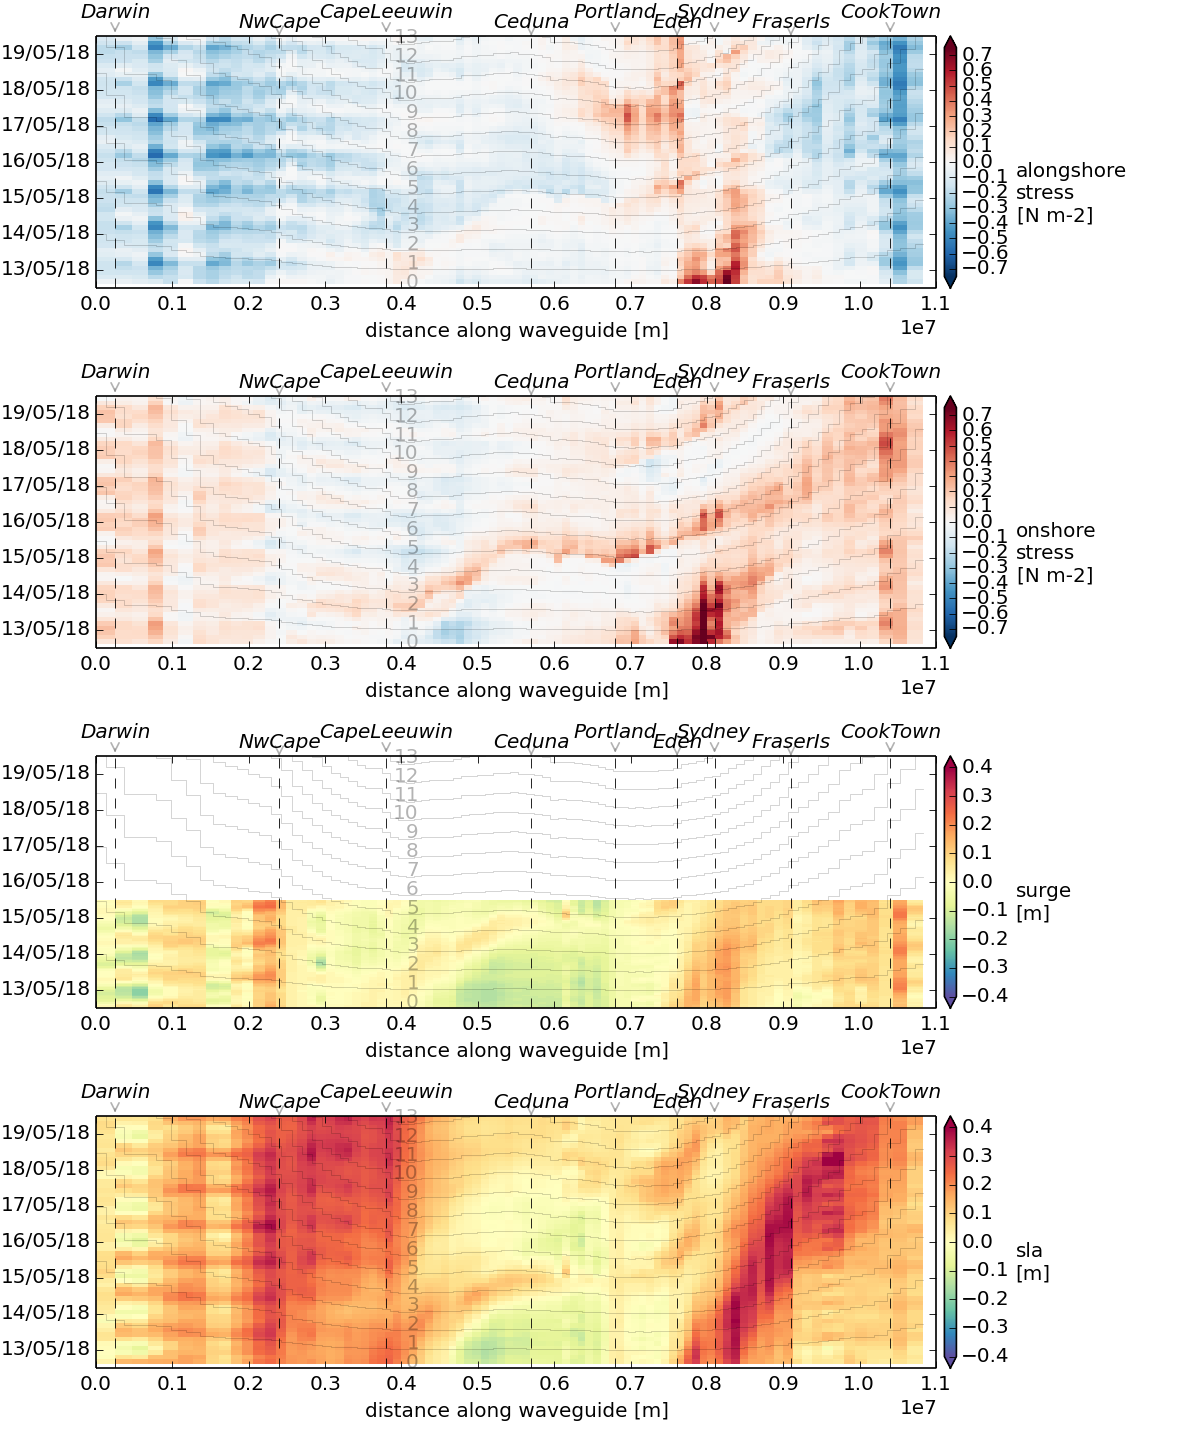
\includegraphics[width=\figwidthFull]{figures/plots/collate_g.png}
    \caption[Forecast with basedate 2018-05-12]
            {A single forecast with basedate 2018-05-12.  Each field is shown on a separate axis with identical time and space limits, feint contours indicate pendulum days to highlight changing inertial periods over the large latitude range. (a) longshore wind stress $\tau_{along}$ units Pa (b) onshore wind stress $\tau_{on}$ units Pa (c) Surge [3-day lead time only] (d) OceanMAPS.}
    \label{fig:collate_g}
\end{figure}  
%----------------------------
\subsection{Forecast differences viewed in waveguide coordinates}

In addition to providing for focused visualisations, this data reduction method facilitates model inter comparisons that target CTW features.
The following examples contrast behaviour of the barotropic surge model with the lower resolution but dynamically rich global ocean forecasts.
Understanding the limitations of dynamic surge forecasts with regard to CTWs has been recently highlighted as important in the Australian context \citep{Hetzel:2018hh}.   


%-------------------------------
\subsection{ Apparent propagation and persistence }
Unlike studies that target the isolation of CTWs \citep{Maiwa2010}, operational users need not distinguish between forced and free propagation as the \emph{apparent} progress of sea level patterns is of primary interest.
Regardless of trapping mechanisms, atmospheric forcing patterns can effectively move around the Australian coast - notably as mid-latitude weather systems travel zonally. 
This movement is reflected by the lagged auto-correlation of wind stress in Figure \ref{fig:Clag0U}.
Apparently anti-cyclonic movement is prominent along the zonally-aligned southern coast but may also occur along non-zonal sections of the coast as patterns of wind alignment progress in time. 
%----------------------------
% correlations
% 0 hours
\begin{figure}[H]\centering
    \noindent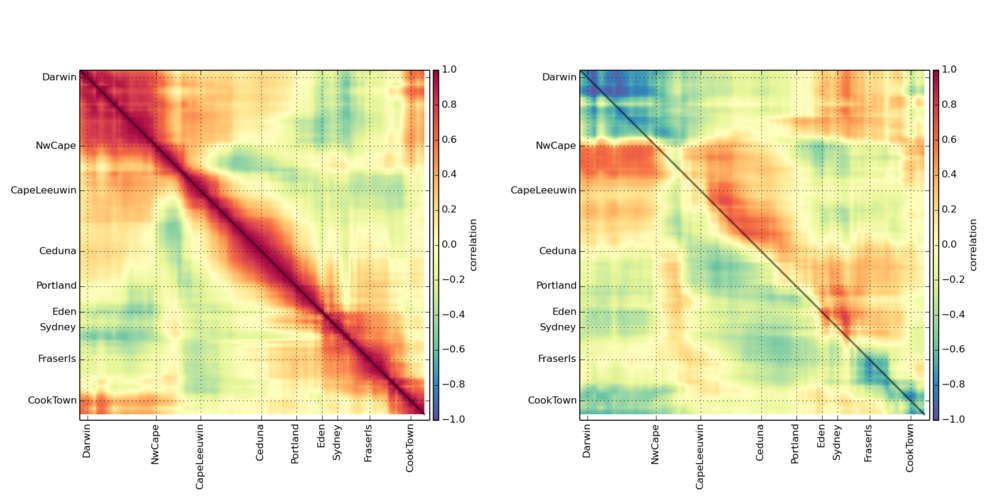
\includegraphics[width=\figwidthBig]{figures/plots/concatC_U_gstr_lag_000.png}
    \caption[Cross-correlation at lag of zero hours $\tau_{along}$]{
             Cross-correlation at lag of zero hours: 
             $\tau_{along}$ lagging (a) $\tau_{along}$ (b) $\tau_{on}$}
    \label{fig:Clag0U}
\end{figure}
%----------------------------
We suggest that a forecast like that shown in Figure \ref{fig:collate_g} may be helpfully narrated as ``a pattern of sea level anomalies moving along the southern mainland and up the NSW coast over the next 7 days'' without any reference to CTWs or physical processes.
Whilst attribution to can aid forecaster interpretation, it is not the primary concern of public narratives.   
 
Inspection of Figure \ref{fig:hov_eg} shows visually coherent structures from which apparent propagation speeds can be derived, corroborating the $\sim$3.4m/s speeds described by \citet{Woodham:2013cl} and others along the east coast.
Though without temporal filtering, faster features more indicative of Kelvin waves ($\sim$25m/s) are also present.   
An implication of Figure \ref{fig:mandelbrot_lengths} is that such speed estimates are dependent on the length scale used to measure the coastal path. 

%-------------------------------
\subsection{ Wind stress orientation and correlation }
Whilst sub-inertial CTW theory is formulated only in terms of longshore winds, the onshore component is also a factor in sea level forecasts \citep{Tilburg:2004cg}.
Propagation of signal along the waveguide means that \emph{non-local} winds can also be important; a fact that we assert is not commonly appreciated by forecasters or the general public. 


Lagged cross-correlations between the datasets projected into waveguide coordinates are relatively simple given that the data are reduced to a common 1D spatial path. 
Some of the structure in these correlations simply reflect details of interpolation and spatial sampling, but meaningful interpretation is still possible; recalling that the same atmospheric forcing is apply to both models.


At zero lag, Figure \ref{fig:Clag0U} provides some indication of typical length scales of the forcing weather systems.  
The peculiar decomposition into longshore and cross-shore directions (wind stress $\tau_{along}$ and $\tau_{on}$) imposed by the geometry of this path realisation is also apparent, with much shorter scales at coastal 'corners' such as Cape Leeuwin.  
Correlations between wind components and modelled sea level at a lag of nearly 3-days are shown in Figures \ref{fig:Clag66sla} and \ref{fig:Clag66surge}.  
Spatially coherent correlation peaks offset to the right of the main diagonal in these figures are interpreted as systematic anti-cyclonic signal propagation. 
Contrasts between the models are evident on the east coast north of Sydney that may reflect the role baroclinic modes.
%-------------------------------------------
% 66 hours
\newcommand\CAPTIONb{Cross-correlation at lag of 66 hours}
\begin{figure}[H]\centering
    \noindent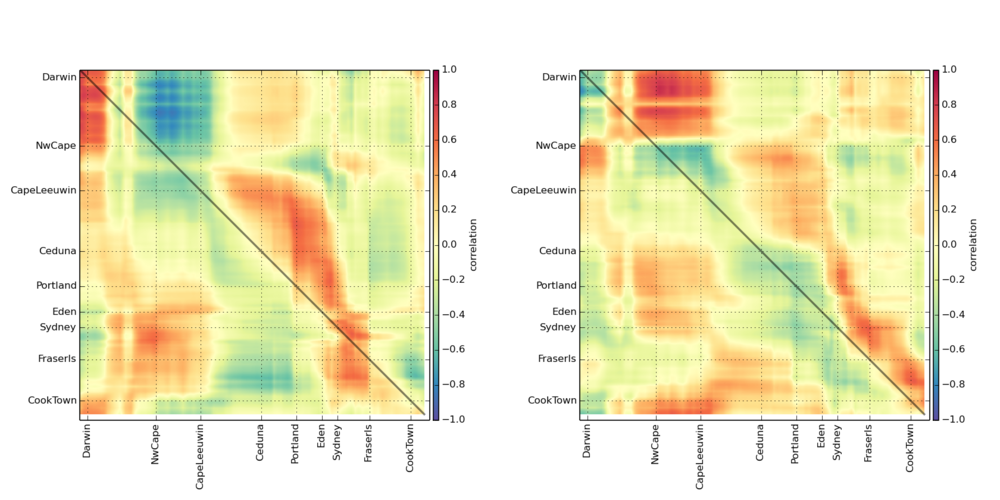
\includegraphics[width=\figwidthBig]{figures/plots/concatC_sla_lag_066.png}
    \caption[\CAPTIONb{} OceanMAPS]{
             \CAPTIONb{}: 
             OceanMAPS response lagging (a) $\tau_{along}$ (b) $\tau_{on}$} 
    \label{fig:Clag66sla}
\end{figure}

\begin{figure}[H]\centering
    \noindent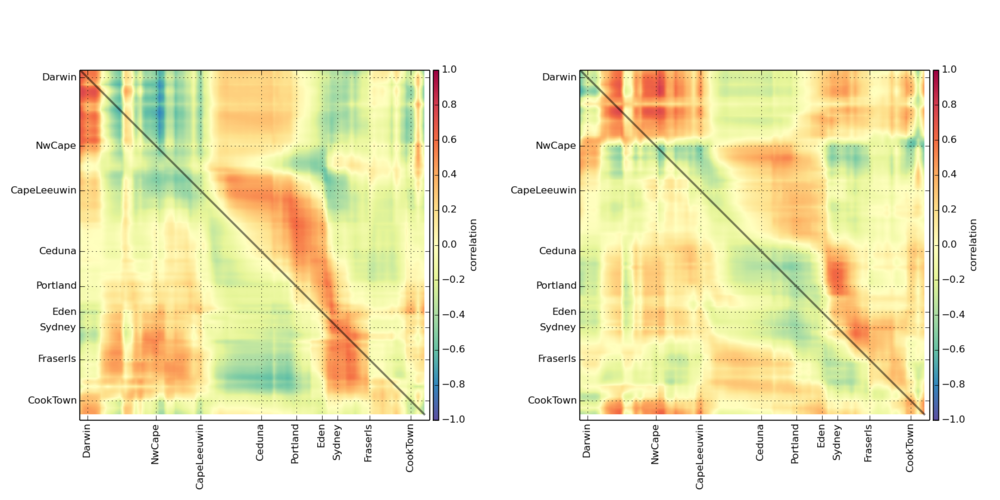
\includegraphics[width=\figwidthBig]{figures/plots/concatC_surgeg_lag_066.png}
    \caption[\CAPTIONb{} Surge]{
             \CAPTIONb{}: 
             Surge response lagging (a) $\tau_{along}$ (b) $\tau_{on}$} 
    \label{fig:Clag66surge}
\end{figure}
%-------------------------------------------


%-------------------------------
\subsection{ Baroclinicity and shelf resolution }
Differences between the interpolated tide observations, OceanMAPS and Surge forecasts are shown in Figures \ref{fig:diff_tide_omaps} and \ref{fig:diff_tide_surge} respectively.
%----------------------------
% differences
\newcommand\CAPTIONc{SLA differences from concatenated datasets}
\begin{figure}[H]\centering
    \noindent\includegraphics[width=\figwidthFull]{figures/plots/interpTdiff_obs_sla_day0_d0.png}
    \caption{\CAPTIONc{} - Tide gauges versus OceanMAPS.}
    \label{fig:diff_tide_omaps}
\end{figure}

\begin{figure}[H]\centering
    \noindent\includegraphics[width=\figwidthFull]{figures/plots/interpTdiff_obs_surgeg_day0_d0.png}
    \caption{\CAPTIONc{} - Tide gauges versus Surge.}
    \label{fig:diff_tide_surge}
\end{figure}

\begin{figure}[H]\centering
    \noindent\includegraphics[width=\figwidthFull]{figures/plots/interpRdiff_sla_surgeg_day0.png}
    \caption{\CAPTIONc{} - OceanMAPS versus Surge.
             Patterns of anticyclonic propagation are apparent and indicative of systemic differences in representation between the models.   
             These features are set against the slower seasonal patterns of difference.}
    \label{fig:diff_omaps_surge}
\end{figure}
%----------------------------
The relative spatial density of available tide gauge data along the east coast is prominent.
Differences between the two models are shown in Figure \ref{fig:diff_omaps_surge}. 
Many of the differences are again simply issues of spatial sampling, especially for the Surge model around the bays near North West Cape.
However structured patterns of difference will at least partially reflect systematic deficiencies in each model.

The relatively large difference between the two forecasts may reflect the lack of baroclinicity in the Surge model.
Dynamics relevant to some forms of CTW propagation are excluded from an ocean model without any buoyancy stratification.   
Apparently propagating patterns of additional signal are present in the OceanMAPS forecasts starting from around Cape Leeuwin.
For instance, the feature on the east coast in mid-May has an apparent celerity of $\sim$3.4m/s; consistent with CTW features reported by \citet{Woodham:2013cl}.


\citet[p.312]{Liao:2018jd} specifically comment that ``...data from the OFAM reanalysis in \citet{Woodham:2013cl} were based on a horizontal resolution of 10km which was not high enough for the Australian east coast ...[and] vertical resolution [details] ... could lead to further inaccuracy in ...CTW amplitude calculation[s].''.
Despite this coarse representation of the narrow east coast shelf, the fact that CTW-like features appear in the OceanMAPS sea level signal, but not in the higher resolution Surge forecasts is interesting and possibly reflects an advantage in allowing at least some representation of baroclinic modes.   
Figure \ref{fig:skill_mebs} summarises and contrasts the SLA forecast skill of the two systems for categorised lead times of 0-24 hours (day-0), 24-48 hour (day-1) and 48-72 hours (day-2).  Day-0 difference data is that shown in Figures \ref{fig:diff_tide_omaps} and \ref{fig:diff_tide_surge}.
On this measure, OceanMAPS notably out-performs the Surge forecast along the east coast from Eden to Fraser Island.
%----------------------------
\begin{figure}[H]\centering
    \noindent\includegraphics[width=\figwidthFull]{figures/plots/plot_skill_path_mebs.png}
    \caption[Forecast skill along the waveguide.]
            {Forecast skill along the waveguide. Mean absolute error for SLA at tide gauge locations. Forecasts are categorised into lead times of 0-24 hours (day-0), 24-48 hours (day-1) and 48-72 hours (day-2).  
            Lower error indicates better overall skill for the 1 year period.
            OceanMAPS outperforms Surge along the populated east coast.
            Forecast skill decay with lead time is evident in both models - except for the apparent unusual inversion in the north west.}
    \label{fig:skill_mebs}
\end{figure}
%----------------------------
As this section of the Australian coast is characterised by such a narrow continental shelf, better skill results from the model with \emph{lower} horizontal resolution is at face-value surprising.  But when this skill is viewed in light of a CTW perspective, it points to the east coast being a region where  propagating sea level signals are significant and where representing baroclinicity provides a tangible advantage to the forecast model.

%--------------------------------------------------------------------------
% Discussion
%--------------------------------------------------------------------------
\section{Discussion}
We assert that a waveguide perspective can provide complimentary insight into the interpretation of daily sea level forecasts and assist in promoting the transfer of research understandings to daily operations.  
Whilst the Australian coastline has been the sole focus of this study, the approach taken could also apply to similar long coastlines, including the Americas and Africa. Whether forecast narratives in those regions also under-play remotely forced coastal sea level is beyond our scope, but a waveguide perspective may offer some insight into explaining the \citet{DiLiberto:2011} finding that a 5-day bias correction improved forecasts skill for particular depth-integrated surge models in a North American context.


The way that numerical forecast guidance is framed informs the forecast narratives that can ultimately influence decisions made at the coast.
Given the apparently common over-emphasis on the role of \emph{local} weather effects on coastal sea level anomalies, a CTW perspective onto sea level forecasts may help direct attention to the relevance of broader longshore patterns and remote winds.
Such a perspective could inform narratives without the need for reference to potentially obfuscating academic terms, for example:
``
...a pattern of sea level anomalies moving up the NSW coast over the next 3 days will raise sea levels... 
''

Beyond the application to daily forecasts, the approach presented will facilitate forecast evaluations that target coastal propagation.
Coastal propagation characteristics are rendered more directly compariable by the reduction of heterogeneous gridded data onto a well-defined 1D waveguide. 
Whilst it is common practice to approach surge forecasting with depth-integrated ocean models, especially in the context of tropical cyclones \citep{Veeramony:2017}, the abilty of models to represent CTWs could have implications for Australian system development priorities. 
Pursuing the work of \citet{Hetzel:2018hh} regarding the (in)adequacy of barotropic ocean models is of particular relevance to the Australian context where the trade-off between representing baroclinic dynamics, spatial resolution and uncertainty is of practical importance.  
     

Improved methods to develop the idea of waveguide coordinates are surely possible.
Sensitivity of the results to waveguide path realisation should be explored and potentially leveraged for specific outcomes.
For instance, to define a coastline that highlights wind orientations of particular significance to driving sea level; extending the manner in which \citet{Tilburg:2004cg} relates measured winds to measured sea level to derive a parametric anomaly forecast model. 


Extension of the 1D approach to also sample model fields along cross-shore profiles (not just at coastal points) could offer insight into the representation of relevant dynamics.
But the algorithm presented is unlikely to be suited to such an extension as it does not provide a conformal map.  Whilst the coordinate directions are orthogonal at the coast, the directions loss meaning with distance offshore to the extent that the profiles can intersect.
  


Well-defined CTW coordinates could in principle facilitate the introduction of process specific numerical models like that of \citet{Brink:1987va} employed by \citet{Liao:2018jd} into the operational setting.
Accurate representation of certain ocean current features in particular could motivate this. 
However, a process-targeted model direction is at odds with the ongoing evolution of increasingly `concrete' generalised simulations \citep{Petersen:2012tr} that are the mainstay of operational forecast centres, so the benefits of a dedicated CTW system would require extraordinary justification.

Forecasts at the coastal interface are both important and challenging. Evaluation approaches that isolate this domain can help align skill metrics with user significance.  
Although not pursued in this discussion, projection of candidate forecast system onto a common wave-guide path will allow for detailed quantitative comparisons of propagation characteristics.  Various signal processing techniques are available to exploit spatially-ordered sets of timeseries data for propagation analysis; though the limitations of complex empirical orthogonal functions described by \citet{Merrifield:1990um} should serve as a general caution about over-interpretation.   


\subsection{ Application to new ESM forecast suites}
....TBC ...update to focus on new and downscaled.


ACCESS-S?



Finally we note that whilst forecasting systems will continue to be updated and extended, the data projection and presentation approaches demonstrated here are model-independent and potentially employed as a generic capability within forecaster visual interface.





		\chapter{Delivering conventional tides to compliment modern applications}
%-----------------------
\begin{quote}
{\small
Using the Australian setting, this chapter asserts that conventional tide prediction services can better compliment modern applications by adopting appropriate data categories for machine-to-machine delivery.  It is written from the premise that the notion of such a service would represent a significant conceptual shift for conventional practice. Furthermore, incremental changes in this direction are feasible and would facilitate future improvements. In putting this case, emphasis is placed on clarifying easily confused tidal concepts and especially on the distinguishing official predictions from physical estimates. Three basic problems are outlined: (1)difference of representational aims from tidal models (2) the risk of double counting and (3) discontinuous evolution of parameters.  Whilst nuanced but known to specialists, each can become significant in certain scenarios for an operational service.  A national automated tidal data service would helpfully distinguish between the well established roles for ``official'' tides, forecasting and various auxiliary applications. Demonstrative evaluations are carried out using an archive of analysis parameters from the Australian National Tidal Unit, ocean circulation forecasts and the TPXO global tide solution. A realistic set of data categories are proposed that would facilitate automated delivery but avoid the pitfalls described.
}
\end{quote}

\label{chp:tideFlavours}
%----------------------------------------------------------
% content variables
%----------------------------------------------------------
% define variables for antt station ids used in figure names
\newcommand{\Ba}{63540}
\newcommand{\Ca}{46290}
\newcommand{\Da}{62430}
\newcommand{\Ea}{62290}
\newcommand{\Fa}{61561}
\newcommand{\Ga}{57720}

\newcommand{\Bb}{529020}
\newcommand{\Cb}{200970}
\newcommand{\Db}{005096}
\newcommand{\Eb}{008314}
\newcommand{\Fb}{523757}
\newcommand{\Gb}{200854}

\newcommand{\Bname}{Mornington Island}
\newcommand{\Cname}{Christmas Island}
\newcommand{\Dname}{Point Murat}
\newcommand{\Ename}{Geraldton}
\newcommand{\Fname}{Cape Jervis}
\newcommand{\Gname}{Lord Howe Island}

%------------------------------------------------
% main
%------------------------------------------------
\section{Chapter introduction}
\label{Sec:intro}
%--------------------------
This discussion makes the case that conventional tide prediction services will better compliment modern forecasting by adopting appropriate data categories for machine-to-machine delivery.  It is written from the premise that the notion of such a service would represent a significant conceptual shift from conventional practice.  Section \ref{Sec:intro} characterises the place of conventional tidal prediction within an operational agency with diverse uses beyond navigation. Three problems for a prospective data service are described; (1) section \ref{Sec:OfficialGlobal} highlights the different representational aims of standard tides and physical tide models with respect to the underlying physics ;(2) section \ref{Sec:DoubleCount} addresses the implications of including meteorologically dominated tides and doubling counting signals in hybrid applications; and (3) section \ref{Sec:Evolution} describes the intentional discontinuities in annual tidal parameter updates across the historical archive of Australian operational data.   Finally Section \ref{Sec:proposed} proposes a minimal set of data ``flavours'' that could help ensure an automated machine-to-machine tide service best compliments the modern requirements. 


\subsection{Modern data micro-services and earth system modelling}
National forecasting agencies are increasingly providing machine-readable online data to support the diverse downstream economy of value-adding applications.
This `micro-service' architecture \citep{BCG2020} is increasingly relevant to government services across the board \footnote{\url{api.gov.au}} and more specifically for tides to the International Hydrographic Organisations navigation-focused exchange specifications \footnote{\url{http://s100.iho.int}}.

 
At the same time, earth system model forecasting continues to increase in sophistication along the dimensions of representational 'concreteness' \citep{Petersen:2012kp}, forecast duration, assimilation of observations and combination into seamless services \citep{BOM2020}.
Within this context, coastal sea level is the subject of a diverse range of productive development activity often centred on high resolution numerical simulations and real-time observations \citep{10.3389/fmars.2019.00437}. 


Despite all the advances in earth system modelling, conventional tide prediction remains a unique and persistent form of forecast that is well-suited to on-demand delivery.  Tide predictions are an input to many systems, have relatively tiny data volumes and are built on a conceptual foundation that allows for cheap synthesis of timeseries at arbitrary times.    There are several examples of on-demand machine-readable tidal data service \footnote{such as  \url{https://tidesandcurrents.noaa.gov/tide_predictions.html}} but nothing yet from an Australian agency and none that are known to distinguish variants for different applications.


Automated delivery of conventional tidal data raises the attractive potential to synthesise tidal timeseries at any arbitrary times as required by an application; whether that time be in the past or the future.   But there is a risk that a naive implementation of such a service may unfortunately re-enforce conceptions that tidal sea levels are an uncomplicated data type without what could be called a range of ``flavours''.
Whilst the precise details of tidal data may be irrelevant for many applications, the following discussion highlights why tidal data would be better treated like other analysis and forecast services by clearly distinguishing some variants or data ``flavours''. 
Appropriate distinction of tidal data types would clarify the compatibility of the content whilst allowing developers and users to remain relatively isolated from backend details and processing improvements on the part of the supplying agency.

%--------------------------
\subsection{Why conventional tide predictions are still relevant}
Given the ongoing advances in both observation and simulation, it would be reasonable to assume that conventional tide prediction services have been rendered redundant; but that is not the case. 
Conventional tidal sea level products are well embedded into coastal economies.   The utility of accurate predictions on a sub-hourly timescale provided over multi-year forecast horizons is unique and this reflects the typical dominance of tidal signals in coastal sea level.
Godin colourfully remarked that when inspecting spectra of observed sea level variability from tide gauges ``the [tidal] constituent lines emerge from the noise background as trees from the grass'' \citep{godin:1972}.
The ability to fit and exploit time-invariant admittance relationships between the patterns of astronomical motions and observed sea level records is an early and great success of mathematical geophysics \citep{Cartwright:2000tt}.  Harmonic tidal analysis derives unique ``\textit{forecasting power.. from the infinite extent of its basis functions} ''\citep{Flinchem:2000kp}.
Conventional products such as tide tables are however so well embedded and useful as to be somewhat taken for granted or used in isolation from other information. 

\subsection{National agency practice and diverse uses}
In Australia, harmonic tidal analysis and prediction have been routine business for government agencies for several decades.  For navigation purposes the Australian Hydrographic Service promulgates an annual official set of port predictions in the form of the Australian National Tide Tables (ANTT) and its software version AusTides \citep{austides}.  AusTides is not an automated data delivery service, but rather stand alone electronic version of the tide tables.  
The majority of the analysis behind the tide tables is carried out by the Bureau of Meteorology National Tidal Unit.  
The analyses are founded on a harmonic least-squares method implemented within a proprietary suite of software that traces a lineage to the Proudman institute \citep{MHL2156}.    
The Bureau and various other state agencies publish annual tide predictions at locations additional to the ANTT. 
This well established practice of routine harmonic tidal analysis and prediction will be called ``conventional''.


The downstream application of these tidal sea-level products is not however limited to navigation.   
In fact, the range of contemporary uses motivates the present discussion; for instance:
\begin{inparaenum}[1)]
    \item land survey and cadastral references - mean sea level and tidal planes such as ``highest astronomical tide'' 
    \item hydrographic survey, charted depths and clearances
    \item long term planning for coastal works and installations
    \item short term forecasts for coastal activities 
    \item filtering (de-tiding) of sea level observations
    \item input into data-driven decision support systems
    \item combination with physical forecasts into seamless water level forecasts 
    \item verification and tuning of hydrodynamic modeling
\end{inparaenum}

A notable aspect of national tide services is the special status of promulgating predictions that have official status \citep{AusNavAct2012}.   For some applications it could be argued this status is more important than forecast accuracy alone.
  

Conventional tidal analysis has some unique and attractive features from an operational maintenance perspective.
At face value, the practice is robust to data-stream indeterminacy,  and has established methods for exploiting heterogeneous, poor quality and historical observations to produce useful predictions.  
Operational support of an annual batch-mode production schedule is far less demanding than real-time continual forecast systems. 
Furthermore, the fact that harmonic methods compress results to a few dozen human-readable parameters that are amenable to routine quality checking and error detection is also operationally attractive. 
Conventional tidal analysis at port locations can be characterised as a slow-motion data-driven method that is somewhat physics-free; especially when compared to modern hydrodynamic simulations. 

Figure \ref{fig:tidePractice} portrays the unique way that conventional tidal practice can transform heterogeneous historical records into a consistent timeseries product at arbitrary time sampling.
The pragmatic role of experts in managing what is now commonly  called ``data wrangling'' and merging non-uniform and auxiliary sources is a notable contrast to fully automated systems.
 
\begin{figure}[!hbt] \centering
        \includegraphics[width=\figwidthFull]{figures/diagrams/tideSchematic.pdf} 
        \caption{Conventional operational tide prediction update process}
        {Schematic illustrates how a conventional tidal process manages heterogeneous data sources on an annual update cycle.  Official tide requirements are not identical to those of all data users.  Dotted lines indicate the potential for on-demand synthesis.}
        \label{fig:tidePractice}
\end{figure}   


Growing access to real-time quality observations both remote and insitu has to potential to tip the balance of value away from conventional tidal and even physical simulations at shorter timescales (eg \citep{10.3389/fmars.2019.00437}, \citep{10.3389/fmars.2020.00260} ), but it will be difficult to displace at the longer scales of months to years that conventional products are relied upon.
Furthermore the pragmatic matters of applying real-time quality control, managing data source inhomogeneity and the relatively sparse spatial coverage remain non-trivial problems in Australia viewed from a a national perspective.


Even if the unique properties of conventional tide products seem to guarantee some ongoing relevance, the following discussion makes a case for ensuring that conventional tide products are delivered in a manner that is fit-for-purpose without inviting needless representational error. 


%--------------------------
\subsection{Precedents for data differentiation}

Most simply, the distinction between a forecast and an ``analysis'' would not be possible if an automated tidal service provided a single all-purpose synthesised signal.
This distinction is obvious to users of weather forecast data and other oceanographic products \footnote{(eg \url{https://marine.copernicus.eu/})} but arguably tidal predictions have to date maintained an exceptional product status.  Tides in general are commonly thought of as being much more akin to astronomical phenomena than oceanographic model outputs \citep{Jay:2003bj} \citep{10.1029/2018rg000636}.


The operational delivery of remote  observations of sea level has well established distinctions between what could be called data `flavours'.   Both with regard to the distinction between rapid update interim products and behind-real-time quality analysis as well as the wide range of geophysical  correction combinations that are suited to different applications ( eg \citep{Scharroo:2014vv} )


Allowing for the effective operational use of standard tide products in the context of satellite observations raises the significance of basic compatibility 
issues such as vertical reference datums \citep{10.3389/fmars.2020.549467}.
Similarly, whilst remote observations of sea level anomalies (SLA) are a critical constraint on operational non-tidal forecasts \citep{10.1080/1755876x.2019.1685834}, any extension to render tide gauge data into the same format would require compatible tidal corrections - and corrections differ in intent from official port predictions.


%------------------------------------------------
\section{Problem 1: different conceptions of tidal}
\label{Sec:OfficialGlobal}
Standard tide predictions and spatial (eg gridded) tide solutions are in parallel use within ocean forecasting but do not aim to represent exactly the same phenomena.    The potential for this to be problematic is apparent in the case of global tide solutions. 
Global tide solutions are a foundational oceanographic product that in rough approximation extends the tradition of tidal analysis well away from tide gauges.   Similar to conventional tidal techniques, these solutions conceptualise the ocean as a linear-time-invariant (LTI) system forced by the tidal gravity patterns. Whilst production of the solution typically involves a hydrodynamic component\citep{Egbert:2002ug}, the result is effectively the spatial equivalent to a set of static conventional tidal parameters.   The surface height predictions from global tide solutions allow for the decomposition of remote ocean observations into tidal and nontidal components, but are also widely used for other extension applications.
In contrast to the advancing ability of physical ocean circulation forecasts to explicitly include tides (eg \citep{10.1016/j.ocemod.2019.02.008}), global LTI tide solutions share the unique ability of conventional prediction methods to efficiently provide data at the arbitrary times required by the application.


For instance, the national inter-tidal extent mapping exercise of \citet{10.3390/rs10030480}  directly applied global model predictions in part for the machine-readable and on-demand availability.
Various Australian studies of water level \citep{Haigh:2013bn}\citep{Pattiaratchi2018} and more recently currents \citep{10.5194/os-2020-107} all apply timeseries synthesised from global model solutions to provide model boundary conditions at what ever time period is required.    Such simulations add value at the time and length scales afforded by higher spatial resolution, but the longer scales require special handling that bring to attention the manner in which the aims of physical models and standard predictions differ.

\subsection{Intentional differences - especially for long period tides}
Harmonic developments of the tidal potential include relatively a weak species referred to as the long period tides.  Some of the long period constituents are known by conventional names such as \textbf{Sa}, \textbf{Ssa}, \textbf{Mm},\textbf{Msf} and \textbf{Mf}; see \citep[table 4]{agnew2015}.
Conventional tidal prediction applies essentially the same statistical fitting procedure to the long period tides as to the more familiar higher frequency tidal periods; though usually with some inclusion caveats based on the observational record. 
But regardless of record length, the treatment of long period tides highlight a difference in the aims of conventional tide prediction and modern tide models.   Namely the extent to which it is desirable to fit patterns that are primarily the result of non-astronomical phenomena.
Parker's tide manual states that ``\textit{whether the calculated values of Sa and Ssa are used or not, becomes almost a philosophical question...and may not represent the annual cycle for a particular year very well anyway}''  \citep[Section 3.7]{Parker:2007wq} 

Physical approaches to the quantifying global long period tides \citep{Egbert:1994wz} do not result in amplitudes anything like those resulting for conventional tide gauge records; especially for when relatively short records and significant nontidal power noise is involved.   Amplitudes of over 20cm are attributed to long period tides in places along the Australian coast as shown in Figure \ref{fig:SaAmp}. In contrast to the aim of physical attribution, when an annual forecast of sea level is the target it is understandable that \textit{any} pattern found to be periodic enough to project onto the tidal basis functions is included in the synthesis of the prediction. 

Even if this intentional difference is known to specialists, downstream users of an automated tidal data service are at risk of building in needless representational error if the distinction is not designed clearly into the service.
The nature of tidal analysis is such that the distinction is best not conceptualised as simply high versus low frequency, but rather physical versus periodic.   The periodic but not gravitationally forced patterns have historically been termed `radiational' tides \citep{agnew2015}.  So the situation outlined for the long period tides also exists for the generally tiny but weather-dominated daily constituent \textbf{S1} \citep{Ray:2004ts}.
 
% Amp
\begin{figure}[!hbt] \centering
    \includegraphics[trim={0 0 0 1cm},clip,width=\figwidthBig]{figures/maps/locations_SaAmp.pdf} 
    \caption{Amplitude of \textbf{Sa} at analysis locations}
    {Amplitude of \textbf{Sa} at analysis locations. Over 650 mixed-quality stations are on record.}
    \label{fig:SaAmp}
\end{figure}

% Pha
\begin{figure}[!hbt] \centering
    \includegraphics[trim={0 0 0 1cm},clip,width=\figwidthBig]{figures/maps/locations_SaPhaAnyM2Update.pdf} 
    \caption{Phase of \textbf{Sa} at analysis locations}
    {Compared to Figure\ref{fig:SaAmp}, only 132 stations have recently updated analyses. Location names used in text are also shown. Note that there are different conventions for allocating Doodson codes that influence interpretation of these phase values \citep[10.4]{PCTMSL-sp9}}
    \label{fig:SaPha}
\end{figure}   

In contrast to conventional tidal analysis, the widely used Oregon State University Tide Prediction Software \citep{Egbert:2002ug} [hereafter \textbf{TPXO}] totally excludes Sa, Ssa, Msf and S1; but both include Mm and Mf.  Subsequently any application that brings both type of prediction into the same context, even if indirectly, requires some caution to avoid representational inconsistency. 


\subsection{Inter-representation agreement}
Given that the signal amplitudes are generally rather small and that most tidal evaluations are carried out in frequency space, the following evaluation aims to demonstrate the practical implications when handling synthesised timeseries.

Variants of 15 minute tide predictions at all Australian sites for the full year of 2020 are used for comparison.   TPXO predictions were generated using the standard interpolation to site locations and sites where excluded that fell beyond the solution grid.   The National Tide Unit in-house software (unpublished) was modified to selectively exclude particular constituents in order to generate alternative ``standard'' predictions for the study period.  All prediction time series for this comparison are relative to MSL (more on that in Section \ref{Sec:MSL}).   Both systems apply so-called nodal or satellite corrections to modulate a finite list of constituent parameters.   

It is to be expected that a global tide solution will not represent all the localised and shallow-water patterns that a conventional analysis can capture.   However the aim of this evaluation is to highlight the arguably less-expected but intentional representational difference for primarily meteorological tides.   To this end a the following timeseries comparison metric is shown on the summary map in Figure \ref{fig:improveOtps}.
\begin{equation}
    I = 1- \frac{rms(\eta_{B}-\eta_{TPXO})}{rms(\eta_{A}-\eta_{TPXO})}
    \label{eq:improvment}
\end{equation}
With water level timeseries $\eta$ variants:
\begin{inparaenum}
[A)]
    \item port tides with all constituents; 
    \item port tides with excluded constituents individually and in combination: Sa, Ssa, Mm, Msf, Mf and S1.
\end{inparaenum}

The \textit{total removal} of the selected constituent terms consistently improves the compatibility of the physical and conventional predictions as is expected.   Moreover, improvement in agreement is partially contributed by each individual constituent with the only case for any ambiguity being \textbf{Mf}; visualised in Figure \ref{fig:improveOtps} panel [b]. Mf is the strongest of the long period forcing terms but still overall these results indicate that the conventional tide attribution is skewed towards the projection of nontidal noise (see Figure \ref{fig:williamsFraction} panel [e] as well). 

As an example of the practical implications of such compatibility, consider the role of conventional tidal planes such as Highest and Lowest Astronomical Tide (HAT and LAT).  Whereas these planes are derived at port locations based on standard predictions that include radiational tides, any spatial extension of the planes that involves a physical tide model risks systematic disagreements of order 10-20cm.  


\begin{figure}[!hbt] \centering
    \begin{subfigure}[b]{\figwidthHalf}
        \includegraphics[trim={0 0 0 1cm},clip,width=\textwidth]{figures/maps/otpsPortCompare_Improve2020_105_diffRmse.pdf}
        \caption{Improvement metric due to all exclusions}
    \end{subfigure}
    \begin{subfigure}[b]{\figwidthHalf}
        \includegraphics[trim={0 0 0 1cm},clip,width=\textwidth]{figures/maps/otpsPortCompare_Improve2020_205_diffRmse.pdf}
        \caption{Same for \textbf{Mf} alone - note scale}
    \end{subfigure}
    \\
    \begin{subfigure}[b]{\figwidthThird}
        \includegraphics[width=\textwidth]{figures/plots/compareTides_\Fa_Full2020.pdf} 
        \caption{\Fname{} comparing standard tides to TPXO}
    \end{subfigure}
    \hfill{}
    \begin{subfigure}[b]{\figwidthThird}
        \includegraphics[width=\textwidth]{figures/plots/compareTides_\Fa_2020_201.pdf} 
        \caption{\Fname{} excluding only annual \textbf{Sa}}
    \end{subfigure}
    \hfill{}
    \begin{subfigure}[b]{\figwidthThird}
        \includegraphics[width=\textwidth]{figures/plots/compareTides_\Fa_2020_105.pdf} 
        \caption{\Fname{} excluding all constituents discussed}
    \end{subfigure}
    
    \caption{Representational agreement between global tide model and port tides}
    {Consistency between TPXO tide model and 'official' port tides is improved by total removal of weather dominated constituents from the later.   Predictions relative to MSL.  Metric is unitless - see Figure \ref{fig:SaAmp} for \textbf{Sa} amplitudes.}
    \label{fig:improveOtps}
\end{figure}   


%------------------------------------------------
\section{Problem 2: double-counting in hybrids}
\label{Sec:DoubleCount}
A practical implication of facilitating downstream applications to access tidal data is the risk of ``double-counting'' signal; especially when hybridising tide data with physical models. 
Williams \citep{10.5194/os-2020-107} described this risk and made evaluations based on the tidal analysis of global barotropic ocean simulations for single one year period. 
The supplementary data supplied by Williams are used to visualise the power projected by wind and pressure effects onto standard tidal constituents in Figure \ref{fig:williamsFraction}.  The spatially consistent high ratios for long periods and S1 stands in stark contrast to the small fractions attributed to the other constituents (not shown).    
For the purposes of providing a tidal data service that can facilitate hybrid applications (eg \citep{Taylor:2017coa}) whilst mitigating double-counting, these evaluations suggest that simply excluding the long periods and S1 in total would be a reasonable starting point.   This is discussed further in  section \ref{Sec:proposed}.
This simple interpretation of the Williams evaluation intentionally underplays the details of phase and wave interaction effects to focus on the gross differences in representational aim between physical models and standard tide predictions. 
The ``\textit{possibility that ... non-tidal power is leaking into the Mm and Mf estimates}'' in this short model analysis is adds to the expectation that such leakage is a dominant effect for many Australian tide prediction sites, especially given that a barotropic ocean model evaluation excludes the role of steric and ocean circulation phenomena projecting onto tide predictions; discussed further in section \ref{Sec:Evolution}.

It is notable that long period signals in Australian sea level studies have always been subject to careful ``non-tidal'' treatment. For instance Haigh \citep{Haigh:2013bn} and Pattiaratchi \citep{Pattiaratchi2018} ensure that long period signals are appropriately filtered, fit or replaced to account for the representational limits of the respective models when interpreting results against observations.

\begin{figure}[!hbt] \centering
    \begin{subfigure}[b]{\figwidthHalf}
        \includegraphics[width=\textwidth]{figures/maps/AustRegionDiff_SA.pdf}
        \caption{Sa}
    \end{subfigure}
    \begin{subfigure}[b]{\figwidthHalf}
        \includegraphics[width=\textwidth]{figures/maps/AustRegionDiff_SSA.pdf}
        \caption{Ssa}
    \end{subfigure}
    \begin{subfigure}[b]{\figwidthHalf}
        \includegraphics[width=\textwidth]{figures/maps/AustRegionDiff_MM.pdf}
        \caption{Mm}
    \end{subfigure}
    \begin{subfigure}[b]{\figwidthHalf}
        \includegraphics[width=\textwidth]{figures/maps/AustRegionDiff_MSF.pdf}
        \caption{Msf}
    \end{subfigure}
    \begin{subfigure}[b]{\figwidthHalf}
        \includegraphics[width=\textwidth]{figures/maps/AustRegionDiff_MF.pdf}
        \caption{Mf}
    \end{subfigure}
    \begin{subfigure}[b]{\figwidthHalf}
        \includegraphics[width=\textwidth]{figures/maps/AustRegionDiff_S1.pdf}
        \caption{S1}
    \end{subfigure}
    \caption{Fraction of tidal amplitude attributed to wind and pressure effects}
    {Data from supplementary material provided by \citet{10.5194/os-2020-107}, based only on amplitude and ignoring magnitudes $<1$cm.  As a starting estimate, the observational-based standard analysis of these constituents could be categorised as primarily non-astronomical.}
    \label{fig:williamsFraction}
\end{figure}

The practical impact of such double-counting is evaluated below using operational sea level data from a system that linearly superposes standard tide parameters with a global ocean circulation forecasts and other inputs at tide gauge locations \citep{Taylor:2017coa}\citep{10.1080/1755876x.2019.1685834}.
Figure \ref{fig:aggStatsComet} summarises the skill impact of applying the full standard tide prediction in place of a physical tide estimate that excludes nominally weather dominated constituents. Figure \ref{fig:aggStatsPdf} shows the day-1 error distributions for the same dataset at two example stations.
For these evaluations no bias correction was applied and sample means over approximately 3 years of 1-hourly data are removed.  Whilst the predictive skill characteristics varies between locations, the change from the double-counting scenario (`A' in the figures) to the physical tide scenario (`B') systematically reduces excess variance and improves correlation.

\begin{figure}[!hbt] \centering
    % Taylor
        \includegraphics[width=\figwidthBig]{figures/plots/taylorDoubleCount.pdf}
        \caption{Forecast skill decay contrasting two tide prediction variants.}
        {Full forecasts based on linear superposition. Summary of the skill impact due to excluding constituents discussed in the text, across many tide gauge locations. Normalised relative to respective observations \citep{Taylor:2000wp}. Each `comet' traces 7 forecast days.  Change from A to B marked for first day.}   
        \label{fig:aggStatsComet}
\end{figure}   

\begin{figure}[!hbt] \centering
    % D
    \begin{subfigure}[b]{\figwidthHalf}
        \includegraphics[width=\textwidth]{figures/plots/ObsError_\Db.png}
        \caption{Day-1 errors \Dname{}}
    \end{subfigure}
    % G
    \begin{subfigure}[b]{\figwidthHalf}
        \includegraphics[width=\textwidth]{figures/plots/ObsError_\Gb.png}
        \caption{Day-1 errors \Gname{}}
    \end{subfigure}
    \caption{Forecast error distribution examples.}
    {Variants shown are [A] all constituents (official) and [B] exclusion of nominally weather dominated (weather-free).  Operational data for $\sim3$ years. Record means removed.} 
    \label{fig:aggStatsPdf}
\end{figure}   


%------------------------------------------------
\section{Problem 3: constants are not really constant}
\label{Sec:Evolution}
The final problem to motivate the proposed split of tidal data service types is the manner in which tidal parameters vary historically with each annual update.
Australian tidal agencies do not systematically publish the parameters associated with the annual tidal production cycle; expect for the subset of constituent values at select sites that are supplied with the nautical publications \citep{austides}.  The following evaluation is believed to be the first account of the temporal evolution of parameters behind these official predictions.  

Conventional tidal parlance reflects an effective aim for the annual analysis that is to better identify a time-invariant admittance relationship characterised by a set of constants; constants that ideally wouldn't change if only we knew them well enough. Flinchem characterises this as old clockwork and  line-spectrum framework \citep{Flinchem:2000kp}. 

In contrast, Colosi and Munk assert that ``\textit{variability in the values of tidal `constants' should be the rule rather than the exception!}'' \citep{Colosi:2006va}
The expectation of temporal instability for tidal constants has recently been further elaborated by  \citet{10.1029/2018rg000636} and \citet{10.1002/2017jc013165} amongst others.    This reasonable characterisation obviously presents some level of conceptual incompatibility with standard practice.

Inspection of annual changes across the archive of analysis parameters first and foremost highlights the wide range of sources and heterogeneous inputs managed to produce tide tables - as characterised in Figure \ref{fig:tidePractice}.    Whilst the ability to derive value from such a range is a great strength of conventional practice, the resulting predictions  should be accompanied by rankable quality measures as proposed in Section \ref{Sec:proposed}.
The evolution of tidal parameters across the archive is addressed below in two parts relevant to a prospective automated tidal data service:  updates to nominally weather-dominated harmonics and then updates to the separation of MSL from prediction datum.

Of all the sites on the archive, only a subset are based on tide gauges stations that are both in operation and supplying data to the agency for analysis. When new observations are available the annual analysis typically extends the length of record analysed.   The analysis of a continually accumulating record is consistent with the aim of better fitting a set of constants; but is in contrast to studies specifically investigating non-stationary tidal evolution such as Devin \citep{10.1002/2017jc013165}.
As an indication of how actively updated tidal parameters actually are, the full set of well over 600 tidal locations was reduced to around 130 that had any change to the 5 significant figures attributed to M2 amplitude since 2011 - this shown by the reduction in sites between Figures \ref{fig:SaAmp} and \ref{fig:SaPha} .


%--------------------------
\subsection{Harmonics}
To illustrate the evolution of nominally weather-dominated constituents, a set of six tide prediction sites spanning the Australia region are selected and detailed in Table \ref{tab:sites}.  The map in Figure  \ref{fig:SaPha} indicates the geographic location of these sites.
Each of these sites have recent forecasting relevance and real time observations but are in some way challenging from a conventional tidal prediction perspective.   These are mainly \textit{secondary ports} in which the observational record is known to be less than ideal. 
Figure \ref{fig:complexEvolution} shows how these `constants' have evolved over the last decade at the selected sites.   Overall the changes reflect the projection of quasi-periodic signals and growing record length.  

%----------------------------------
% table
%\begin{specialtable}[H]\centering
\begin{tabular}{ r|p{1cm}|p{1.2cm}|c|c|c }
Name 
 & ANTT 
 & BoM 
 & web  
 & port type
 & Obs for 2022
  \\ 
\toprule
Mornington Island 
 & 63540 
 & 529020 
 & Y 
 & Secondary 
 & 30/06/2007 - 31/12/2016
 \\
Christmas Island  
 & 46290 
 & 200970 
 & Y 
 & Secondary 
 & 04/08/2009 - 31/12/2018
 \\
Point Murat       
 & 62430 
 & 005096 
 & Y 
 & Secondary 
 & 13/05/2008 - 31/12/2019
 \\
Geraldton         
 & 62290 
 & 008314 
 & Y
 & Primary   
 & 01/01/1985 - 31/12/2019
 \\
Cape Jervis       
 & 61561 
 & 523757 
 & N 
 & Secondary
 & 29/05/2014 - 31/12/2019
 \\
Lord Howe Island  
 & 57720 
 & 200854  
 & Y 
 & Secondary 
 & 02/08/1994 - 31/12/2019
 
 \\
\end{tabular}
\label{tab:sites}
\end{specialtable}
 
\begin{table}\centering
\begin{tabular}{ r|p{1cm}|p{1.2cm}|c|c|c }
Name 
 & ANTT 
 & BoM 
 & web  
 & port type
 & Obs for 2022
  \\ 
\hline
Mornington Island 
 & 63540 
 & 529020 
 & Y 
 & Secondary 
 & 30/06/2007 - 31/12/2016
 \\
Christmas Island  
 & 46290 
 & 200970 
 & Y 
 & Secondary 
 & 04/08/2009 - 31/12/2018
 \\
Point Murat       
 & 62430 
 & 005096 
 & Y 
 & Secondary 
 & 13/05/2008 - 31/12/2019
 \\
Geraldton         
 & 62290 
 & 008314 
 & Y
 & Primary   
 & 01/01/1985 - 31/12/2019
 \\
Cape Jervis       
 & 61561 
 & 523757 
 & N 
 & Secondary
 & 29/05/2014 - 31/12/2019
 \\
Lord Howe Island  
 & 57720 
 & 200854  
 & Y 
 & Secondary 
 & 02/08/1994 - 31/12/2019
 \\
\end{tabular}
\caption{Selected tidal stations for focus.}
\label{tab:sites}
\end{table}

%----------------------------------

\begin{figure}[!hbt] \centering
    % B
    \begin{subfigure}[b]{\figwidthHalf}
        \includegraphics[width=\textwidth]{figures/plots/complex_\Ba.pdf}\caption{\Bname{}}
    \end{subfigure}
    % C
    \begin{subfigure}[b]{\figwidthHalf}
        \includegraphics[width=\textwidth]{figures/plots/complex_\Ca.pdf}\caption{\Cname{}}
    \end{subfigure} 
    \\
    % D
    \begin{subfigure}[b]{\figwidthHalf}
        \includegraphics[width=\textwidth]{figures/plots/complex_\Da.pdf}\caption{\Dname{}}
    \end{subfigure}
    % E
    \begin{subfigure}[b]{\figwidthHalf}
        \includegraphics[width=\textwidth]{figures/plots/complex_\Ea.pdf}\caption{\Ename{}}
    \end{subfigure}
    \\
    % F
    \begin{subfigure}[b]{\figwidthHalf}
        \includegraphics[width=\textwidth]{figures/plots/complex_\Fa.pdf} \caption{\Fname{}}
    \end{subfigure}
    % G
    \begin{subfigure}[b]{\figwidthHalf}
        \includegraphics[width=\textwidth]{figures/plots/complex_\Ga.pdf} \caption{\Gname{}}
    \end{subfigure}
    \caption{Evolution of select tidal constituents at focus sites.}
    {Histories of annual updates for sites listed in table \ref{tab:sites} displayed as both phasors and smaller timeseries of amplitude and phase.  Annual results are not independent due to accumulating input data. Relatively radical changes reflect the power of quasi-periodic variability at these frequencies as well as the heterogeneous record quality on which analyses are based} 
    \label{fig:complexEvolution}
\end{figure}   

Of the constituents shown, the annual signal \textbf{Sa} is dominant at all of the sites.
Intra-seasonal power and variability is notable at the two sites located in the North West; Port Murat and Christmas Island.   The existence of long period ocean phenomena in this region associated with the MJO atmospheric forcing described by \citeauthor{Maxime:2019jc} should be expected to project onto a conventional tidal analysis.   Internal-tides are of special interest on the North West Shelf \citep{10.3389/fmars.2021.629372} and may also play a role in  modulating surface water level patterns in the manner described by \citeauthor{Colosi:2006va}.

Of the selected sites, Geraldton shows the smoothest and least significant changes.  Given that it is both a \textit{primary port} and based on the longest observational record it may at face value appear to represent the true tidal pattern. But the strong seasonality of the Leeuwin current described by \citeauthor{Ridgway:2004kb} provides an attribution that relies neither on the gravitational tidal forcing nor a barotropic ocean response to weather forcing. % NOTE - anything about the tide gauge boat impact  to add?
This connection is supported by recent attribution studies of sea level along the WA coast, in which historical observations are decomposed using a hybrid tidal and filtering approach to highlight the ``\textit{interesting connection between the probability of extreme sea level events with the large-scale dynamics of an ocean boundary current system}'' \citep{10.1029/2020ef001620}.

Lord Howe Island is located within the eddy the field associated with the East Australian Current and subject to relatively powerful and slow sea level variations.    The parameters fit by the standard tide prediction are quite small and would appear to thus be correctly rejecting the projection of these  non-periodic variations.   However, this site is has been recorded as problematic for the utility of some tide predictions ``\textit{...due to persistent yet sporadically changing ocean levels ...at similar frequencies to the Sa and Ssa constituents [such that] forecasting can then result in errors greater than the actual residual}''\citep{MHL2156}.  The problematic predictions were not based on the analysis of the NTU but rather on a practice of fitting tides to shorter records motivated by the aim of better prediction a useful mean sea level (MSL) for year ahead in the context of inter-annual variability.

%--------------------------
\subsection{Mean sea level}
\label{Sec:MSL}
What mean sea level (MSL) represents for operational purposes and across applications has been single out as a source of inter-agency inconsistency \citep{MHL2156}.
For studies of sea level average return periods, \citeauthor{Haigh:2013bn} considers MSL to be a time varying background sea level signal.
In contrast, for spatial and survey applications MSL is an important geodetic reference treated as as a static value. Furthermore the decomposition of a static MSL to quantify the mean dynamic topography component has a special relevance for datum unification \citep{Filmer:2018cu}.
Applications of tidal predictions that project to periods well beyond the current year such as that described by \citeauthor{10.1007/s11069-021-04600-4} require the ability to separately account for any MSL component.
The official Australian nautical predictions are accompanied by an explanation that highlights to overlap between the concept of MSL and long period tides:
``\textit{Wherever possible, predictions are based on continuous observation of the tide over a period of at least one year, in such cases the average changes in mean sea level due to changes in meteorological conditions for the year in question are calculated and included in the predictions.  These changes do not, however, repeat themselves exactly from year to year; it has been advisable, therefore, to observe and analysis changes in mean sea level for a period of not less than three years.   In case of modern analyses, this practice has been increasingly adopted}'' \citep{austides}

The elevation of MSL relative to \textit{prediction datum} (PD)is updated annually for Australian predictions for multiple reasons.   One is to account for global sea level trends across the prediction sites inclusive of locations for which no recent observations are available.   Other reasons include the redefinition or relocation of PD at a port.  Figure \ref{fig:z0Evolution} summarises the actual historical 
changes in this offset across all Australian primary and secondary ports relative to the arbitrary reference year of 2011.   It is evident that older predictions and lower quality secondary ports are most susceptible to larger step changes.

\begin{figure}[!hbt] \centering
    \includegraphics[width=\figwidthFull]{figures/plots/Z0_evolution.pdf}
        \caption{Evolution of zero frequency levels used for annual tide predictions at primary and secondary ports.}
        {Changes are shown relative to arbitrary zero year of 2011. Variations reflect the heterogeneity of sources and potential for offset discontinuities with on-demand data delivery}
    \label{fig:z0Evolution}
\end{figure}   

\subsection{Relevance of annual updates for a data service}
The annual update to official parameters is undertaken with the specific goal of improving stand-alone water level predictions for the year ahead.  It should come as no surprise that this practice may introduce discontinuities when looking back over historical predictions.
But looking back at official data is exactly what some users of an automated data service may require and it is important that there is no confusion about what data is being supplied.
Compare this to an application where the aim is simply to estimate the tidal water level variability component  for a historical period regardless of what was official or available at the time.
Figure \ref{fig:tideHistoryTs} illustrates the difference for the case of  \Dname{}.  The evolving long period characteristics of the official annual updates can be compared to panel [c] in Figure \ref{fig:complexEvolution} recalling that these operational values represent a growing input record and a independent observations such in the studies of Devin \citep{10.1002/2017jc013165}. 

\begin{figure}[!hbt] \centering
    \includegraphics[width=\figwidthFull]{figures/plots/piecewiseTide_62430.pdf}
        \caption{Contrast between concatenated standard predictions and a hindcast.}
        {Site \Dname{}. The hindcast shown is based on the approximate ``weather-free'' tidal parameters.  Note the intentional discontinuities in official predictions associated with annual updates and growing input record length.}
    \label{fig:tideHistoryTs}
\end{figure}   

%------------------------------------------------
\section{Proposed split of routine tidal content}
\label{Sec:proposed}
The above sections have characterised the place of conventional tidal practice alongside operational oceanography within a forecasting agency and described three problems that could impact the value of a singular implementation of a machine-readable tidal data service.   From this starting point, the current section proposes a direction by which the conventional service may incrementally adapt to modern requirements.  This proposal is written from the premise that the very notion that anything other than a singular tide prediction is required represents a significant conceptual shift for conventional practice.
Adding any complexity to operational systems is generally undesirable and a good data service just ``does what it says on the box''.  But considering the diverse uses for synthesised tidal signals and the problems outlined above, the following aims for a data service are put forward: 
\begin{itemize}
    \item deliver tide data valid for arbitrary times
    \item isolate users from details of backend software 
    \item distinguish a physical tide estimate from standard predictions
    \item allow for differentiation between forecasts, hindcasts and analyses
    \item explicate reference datum and MSL change components
    \item provide rankable quality measures
\end{itemize}

With these motivations in mind, a minimal set of tidal data categories are proposed and listed in table \ref{tab:typesSummary}.   Emphasis is placed on conveying the need for \textit{any} signal split rather than exact wording and finer details.  Importantly, such a change could be made as an incremental shift without significant technological change; but would open the path to ongoing improvements in the respective categories. 
Each is discussed further in the subsequent sections.

%\begin{specialtable}[H]\centering
\begin{table}[H]\centering
    \begin{tabular}{ |c|c|c|c|c| }
    \hline
    name    & 
        default reference  & 
        issue date         & 
        valid time limits  \\
    \hline
    standard tide prediction [\ref{Sec:flavour1}] & 
        chart datum & annual & 
        concatenated bounds\\
    \hline
    physical tide prediction [\ref{Sec:flavour2}]& 
        MSL       & 
        arbitrary & 
        no limit \\
    \hline
    physical tide analyses [\ref{Sec:flavour3}]& 
        MSL       & 
        arbitrary & 
        within observation range \\
    \hline
    \end{tabular}
    \caption{Summary of proposed timeseries data categories; metadata are addressed in \ref{sec:spatial} and \ref{sec:quality} }
    \label{tab:typesSummary}
%\end{specialtable}
\end{table}
These proposed incremental changes for the conventional service should not be confused with the vital role of global repositories of sea level observations \footnote{such as \url{www.gloss-sealevel.org}, \url{uhslc.soest.hawaii.edu} and \url{www.gesla.org}}.    The starting premise of this discussion is the ongoing and embedded role of the national agency for conventional tidal services.    
Similarly, global simulation repositories like that described by \citeauthor{10.3389/fmars.2020.00263}
serve an important but different role.

%------------------------
\subsection{Standard reference predictions}
\label{Sec:flavour1}
Standard tide predictions have an official legal status both directly for navigation purposes and indirectly for some other applications.   
For instance the Australian Navigation Act \citep{AusNavAct2012} details a requirement for vessels to carry nautical publications, and specifically tide tables, from the official charting authority.  Charted depths are defined relative to a datum generally aligned with the Lowest Astronomical Tide value derived from synthesised official tidal timeseries over a fixed period \citep{PCTMSL-sp9}.
%Official predictions are forecasts that aim to represent the total still-water level under average conditions. ``\textit{As predictions are given for average meteorological conditions it follows that when conditions are not average the actual tides may differ from those predicted.}''\citep{austides}
Official predictions traditionally cover a fixed validity period of one year and are issued on an annual update cycle well in advance; for instance the 2022 predictions may be issued in late 2020.  An on-demand data service should allow users to access these predictions at arbitrary timestamps within the validity period, and conventional needs such as high and low waters just represent a special timeseries subset.
As described in section \ref{Sec:Evolution}, discontinuities should be expected between these annual official predictions. 
Providing access to \textit{historical} predictions therefore requires a data-service to appropriately handle the forecast validity dates.  Whilst this requirement precludes the use of a single set of tidal parameters to synthesise a hindcast on-demand, it does not rule out on-demand synthesis in general.
Tidal planes associated with official predictions, such as LAT and HAT, should similarly be accessible according to validity period.

%------------------------
\subsection{Physical or `weather-free' tidal timeseries}   
\label{Sec:flavour2}
As described in the preceding sections, there are valid use-cases for tide predictions that do not align with the aims of standard products;  both with respect to the ``official'' status of the annual promulgation and as well as the component of observable sea level that is being targeted.  It is asserted that many such cases require the best available estimate of the tidally-driven component of total sea level.  
Following the evaluations in sections \ref{Sec:OfficialGlobal}and\ref{Sec:DoubleCount} it is asserted that a reasonable approximation to such a physical prediction could be made with existing methods by bluntly removing tidal constituents that are determined to be weather-dominated; specifically all of the long period tides and S1.   Such an approximation is proposed as an adequate and immediately available tidal variant that could be refined in isolation to official prediction constraints. Furthermore, the role of charting PD is unlikely to be relevant to these applications and should be default be excluded.
There is no reason to restrict the refinement of analysis parameters to an annual update cycle.
Such a prediction is simply what physical oceanography has largely thought of as `tides' for decades \citep{Munk:1966ts} despite the fact that response method techniques ``\textit{...have never been adopted for ordinary tide-table production [and] remain essentially a research tool for specialists}''\citep[p.198]{Cartwright:2000tt}.
Combination with dynamic model forecasts requires such a prediction \citep{Taylor:2017coa}, as does any data-driven methodology that involves the filtering of real-time tide gauge observations in order to assimilate non-tidal residuals \citep{10.3389/fmars.2019.00437}. Furthermore, residuals derived using such a weather-free tide prediction prima facie share the representational targets of sea level anomaly (SLA) data derived from satellite altimetry as discussed section \ref{Sec:OfficialGlobal}.
      
%------------------------
\subsection{Behind-real-time quality tidal timeseries}  
\label{Sec:flavour3} 
Whereas a tidal hindcast can be synthesised for a past period with no methodological difference to a forecast, there is a reason to conceptually separate this from an analysis timeseries. The dual meaning of 'analysis' for both the tidal process and the timeseries here is unfortunate but unavoidable and hopefully clarified by context. 
The distinction being analogous to that between a weather model forecast and analysis, or the IGDR and GDRs of satellite data \citep{Picot:2003tp}.    As a starting approximation this data category would be served by conventional methods but only valid for the time span of the input observations. 
Distinguishing this data category would serve the role of a de-tiding filter for historical observations, as an evaluation target for behind-real-time regional tide modelling like that of \citeauthor{10.5194/os-2020-107} and potentially as an input to geophysical re-analysis (eg \citep{10.1029/2017jc013685}).    
In contrast to the use of a constant set of tidal parameters to synthesise a prediction or hindcast, keeping this category separate would allow for the application of non-stationary methods to account for modulation and transient phenomena that can still be usefully attributed to tides as per the discussion of wavelet and other techniques by \citeauthor{Flinchem:2000kp}. 

%------------------------
\subsection{Spatial metadata and levels}
\label{sec:spatial}
Metadata regarding the location, identity and especially relative elevation of tidal timeseries is fundamental to any data service.
Vertical datum transformation and unification is an active area of development is Australia and described by  \citeauthor{Keysers:we} and \citeauthor{Filmer:2018cu} amongst others.   Spatial reference developments such as the Australian Vertical Working Surface are notably also connected to tidal observations \citep{AVWS2021}).   The details are beyond the scope of the present discussion, but the relationship between prediction datum and the ellipsoidal references employed in modern positioning\footnote{\url{ https://www.icsm.gov.au/what-we-do/aushydroid}} is highlighted as carrying special relevance.

%------------------------
\subsection{Rankable quality measures}
\label{sec:quality}
Whilst high quality, continuous long records of sea level observation represent an ideal for conventional tidal methods, in practice this is only available for a relatively small network of tide gauges.   
The schematic in Figure \ref{fig:tidePractice} conveys the attractive ability of conventional tidal practice to produce uniform outputs from a very heterogeneous set of inputs.
Uniformity of format is not the same as uniformity of quality, but without appropriate supporting information users of tidal data would be left to treat all predictions as equal.  

Australian systems currently have effectively only two quality categories: `primary' and `secondary' \citep{austides} that are sometimes also designated `standard' and `subordinate'  \citep{PCTMSL-sp9}.   
It is also common to see unofficial tide predictions clearly marked as ``not for navigation'' to indicate a status other than official.
This binary classification is not sufficient for many applications and it is asserted that the major deficiency is the lack of ability to rank by quality.   There are several dimensions by which synthesized tidal timeseries could be assigned rankable quality measures.    
The analysed observational record length is at least one practical candidate and specifically highlighted by \citeauthor{MHL2156}. But the bespoke analysis process, for instance involving inference or moved stations \citep{godin:1972}), can render record length more ambiguous than at first may be apparent.    
Related to record length is the candidate measure of extrapolation time, to quantify the time period prior-to or after the analysed observational record.     
A quality measure that reflects skill relative to an independent period of water level observations could also provide useful guidance to users of the data.    In contrast, any measure derived directly from the tidal analysis itself (inversion) would require care to avoid over-fitting and the type of circular reference described by  \citeauthor{Thompson2019}. 

The absence of rankable quality measures left \citeauthor{10.5194/os-2020-107} to rely on a needlessly empirical blacklisting procedure to reject tidal analysis sites from a simulation evaluation on the basis of being of grossly poor quality. Such information should readily accompany machine-readable tidal data.

%------------------------------------------------
\section{Concluding discussion}
\label{Sec:Discussion}
This article has put the case that an appropriate clarification of tidal data types and aims will enable a conventional tide prediction service to better compliment a range of modern applications; and that such a change could be relatively incremental and feasible with existing technology. 
There is of course a very long history of proposals for refinements or up-ending of tide prediction techniques \citep{Cartwright:2000tt}\citep{Jay:2003bj}, but this is in contrast a proposal for an incremental shift in thinking for an established and valuable \textit{service}.
The magnitude of the signals and discontinuties are overall rather small at only $\sim10-20cm$.   But scales like this are worth some attention when considering the operational role for forewarning of nuisance flooding \citep{Devlin:2017hu}\citep{10.1071/es19024} and in potentially in complimenting future remote observation platforms \footnote{\url{auswot.org}} and coastal forecasting \citep{10.3389/fmars.2019.00437}.

This proposal has intentionally not promoted the promulgation of tidal analysis parameters and has instead focused on the value of timeseries.   Whilst the publication of parameters would of itself be desirable in terms of transparency, these are less likely to directly deliver the value required by downstream applications.    Most simply because the interpretation and application of tidal constants requires consistency between the analysis and synthesis software. Consider for instance the inconsistent designation of \textbf{Sa} to Doodson numbers \texttt{[0 0 1 0 0 0]} and \texttt{[0 0 1 0 0 ‐1]} between tools \citep{PCTMSL-sp9}.  Let alone the manner in which energy is variously projected onto named constituent groups as a function of record length.  
Providing timeseries would directly serve many direct downstream applications as well as allowing specialist users to `back out' parameters in their own analysis framework as required and in isolation from the details of tools in use by the supplier.

		\chapter{Conclusion}
\label{chp:conclusions}
This desktop study was motivated by the consideration of sea level from within the Australian Bureau of Meteorology, and certain conceptual problems identified behind operational developments.
Exploration of the intersection of conventional tide prediction and operational mesoscale ocean forecasts within the agency has highlighted nuanced issues of representation, system compatibility and user expectation that are relevant to the strategic direction towards ``seamless'' services.
As such, all evaluations treated here have intentionally not pursued higher fidelity coastal simulations, but instead directed attention to some less-studied aspects of evaluating and exploiting predictability with established operational systems.   

As a thesis with publication, much of the body of this document has been published as, or is in preparation for peer-reviewed academic papers.
%------------------------
\section{Findings summary}
In answer to the research questions posed in chapter \ref{chp:introduction},  the findings of this thesis are summarised as follows:\\

Firstly, it was demonstrated that incompatible definitions of ocean ``tide'' are in parallel operational use.
Whereas downscaling for coastal sea level forecasts is clearly a productive approach, mesoscale ocean forecasts can immediately and directly provide significant but qualified forecast value for coastal sea level.
The fact that nominally tidal signals are present in mesoscale non-tidal ocean simulations means that care is required to avoid misinterpretation.

An aggregation approach that combines existing heterogeneous data but accounts for double-counting provides an important skill benchmark for future sea level forecast system development.
The point-based bias correction characteristics from these aggregated forecasts indicate that coastally contiguous extensions to model aggregation may be feasible.


In the operational context of combining and upgrading forecast models, it was shown that the coastal propagation characteristics of candidate forecast systems can be usefully evaluated and compared in a grid-independent waveguide projection.
Such a coastal waveguide projection also offers a means to direct forecaster attention to signals of special relevance along the Australian mainland coast.

Finally, it was argued that conventional harmonic tide predictions are not redundant, despite the ongoing advances in hydrodynamic simulation,  but that operational tide services require appropriate product differentiation to compliment modern applications and facilitate future refinement.
     % <<-- external file

%------------------------
\section{Heterogeneous simulations and seamless services}
The original coinage of "seamless" prediction in the context of climate projections has evolved to now encompass the more general goal of prediction across time and length scales \citep{10.1127/metz/2020/1048}.
Indeed the development of more seamless services is a strategic goal of the Australian Bureau of Meteorology \cite{BOM2020}.
\cite{10.1175/bams-89-4-459} illustrated the concept with a schematic chain of scales reaching from the small and fast out to the large and slow.
The present focus on sea level forecasting allows for a twist on the chain image to highlight the unusual place in which the LTI tidal admittance approach can be located relative to the geophysical fluid suite of simulations.
Figure \ref{fig:forecastScalesChain} schematically shows that tide prediction in general can provide very long horizon prognoses of short time scale fluctuations in sea level; of course subject to many caveats.
%------------------------------
\begin{figure}[h]\centering
        \includegraphics[width=\figwidthFull]{figures/diagrams/scales_with_chain.pdf} 
        \caption{Tide prediction can sit awkwardly with the seamless chain-of-scales analogy and highlights an ongoing role for system heterogeneity; following Figure \ref{fig:forecastScalesAll} and \citep{10.1175/bams-89-4-459}}
        \label{fig:forecastScalesChain}
\end{figure}
%------------------------------
The intention behind this imagery is to emphasise that multi-scale prediction need not be shoe-horned into the tidy cascade of a single consistent earth system simulation framework.
Although a consistent framework and a single simulation code-base is very attractive on multiple fronts  \footnote{\url{https://research.csiro.au/access/what/}}, consideration of the status of sea level and tide prediction provides at least one case in which some sort of exception is sure to be required based on the unique value offered by particular mechanisms and legacy products.  

Operational forecasting today, when viewed holistically, is based on a suite of systems that are not cleanly compatible.
The prognostic potential of Australian Bureau of Meteorology has arguably not been fully realised to some degree as a result of system heterogeneity.  Consider how the forecast information published variously as maps of non-tidal sea level anomaly, storm surge warnings and tide-table products cannot self-evidently be synthesized and directly interpreted in relation to observable sea level.
And whilst progress towards ever more concrete and consistent earth simulations will continue apace, there is sure to be an ongoing operational requirement to handle inhomogeneity and system transitions in manner that actually provides useful forecast value. And in line with the final recommendation of \cite{10.1175/bams-89-4-459}, realising that value will require ``\textit{closer and wider cooperation between the scientific community, stakeholders, policy- and decision-makers to ensure that sea level products are accessible and are used correctly and appropriately...}''. 

%------------------------
\section{Next steps}
The will be ongoing opportunities to improve sea level forecast services as the operational suite of simulation systems improve, but any innovation will necessarily be interpreted by users against the background of conventional tide predictions.

Whilst this body of work intentionally restricted focus to the Australian setting, some of the higher level  characterisations will be translatable to other shores.  Especially the basic conceptual overlap between aspects of conventional tide prediction and hydrodynamic simulation.
The federated jurisdiction combined with the vast expanse of the Australian coast tips the balance of operational challenges towards delivering a more universal, as opposed to highly targeted, approach to forecasting.   As a jurisdictional contrast is available in the case of South Korea, where a dense network of weather and marine observations are maintained under the same auspices as the forecasting agency (eg   
\citep{10.1007/s10236-015-0820-3}).
The vast Australian coast also raises the significance of large scale coastal propagation, and moreover highlights the problem of observation sparsity.


There remains a primary role for \underline{tide gauge observations} to underpin sea level forecasting across the board.
Expansion of the observation capabilities to new platforms, be it video \citep{10.1175/jtech-d-18-0203.1} or wide swath altimetry, will not side-step the ongoing role for tide gauges.
\cite{Keysers:we} emphasised the need for not only a denser network of observations around the Australian coast, but a national repository and ongoing curation of sea level observations and survey connections to support the needs of precision positioning.   
That call is effectively mirrored for forecasting applications in the recommendations of \cite{10.1175/bams-89-4-459}.
As yet, there is no such Australian coordination; at least not in the sense of seamlessly serving real-time and survey applications.
There is an obvious opportunity to better align the capabilities of the conventional tide service, operational forecasting and spatial survey to maintain a foundational public resource.  Whilst small steps have been taken in that direction by the Intergovernmental Committee on Surveying and Mapping \footnote{\url{https://www.icsm.gov.au/}}, progress would be a great enabler for improved sea level forecast services.





Finally, consideration of how tides and sea level fit within the operational setting of the Bureau of Meteorology corroborates the need for a concept of forecasting services that juxtaposes the chain-of-scales model; namely the so-called `micro-service' architecture \citep{BCG2020}.
Quite apart from the vision for an all-encompassing multi-scale earth system simulation, the extraction of value from forecasts more generally appears to be on a fast trajectory towards the downstream combination of heterogeneous inputs for bespoke decision support applications.
Ensuring that forecast outputs of all sorts are machine-readable, discoverable and well-characterised will facilitate the development of improved sea level applications both within and external to the operational agency itself.    

%is increasingly relevant to government services and is embodied by programs such as  \url{api.gov.au}) and the International Hydrographic Organisations  navigation-focused exchange specifications (\url{http://s100.iho.int}).




	\end{mainmatter}
	
	%---------------
	% bibliography
	%---------------
	\addcontentsline{toc}{part}{Bibliography}		
	\bibliography{bib/references_update}
	%---------------
	% appendices
	%---------------
    \addcontentsline{toc}{part}{Appendices}
    \begin{appendix}
		\chapter{More on tidal formalisms}
\label{appendix:tideFormalisms}
\section{Response}
Godin \citep{Godin:1991vx} describes the response method as a cross spectral analysis; whereby a LTI model is inverted from comparison of the input and output timeseries.   
Whereas harmonic methods evolved well before the availability of machine computers, the response method relies on computational signal processing with discretely sampled and finite length time series.
A response analysis aims to empirically characterise the LTI as a complex-valued transfer function on the basis of output coherence with the input/s. 
\begin{quotation}
The goal of any response formalism is to accurately predict the ocean tides by an optimum smooth function, realising that the ocean tides are mostly, although not completely, predictable.
\end{quotation}
The outcome of a response analysis is not a single admittance curve, but rather a small number of distinct curves; typically the semi-diurnal, diurnal and long-period tides associated with degree-2 spherical harmonics $(n,m)=(2,2),(2,1),(2,0)$.\\
Smoothness of $Z(\omega)$ within each distinct tidal band is a core principle behind methods for determining admittances.  
\begin{align}
    \label{E:response}
    g(\Delta t) + \dots &\Rightarrow & \fbox{empirical admittance curves $Z$} &\Rightarrow & \mbox{$\eta(\Delta t)$}  %\nonumber
\end{align}
Where $g(\Delta t)$ is a discretely sampled input signal, nominally the equilibrium tide.   Figure \ref{fig:response} schematically illustrates the process.
Once determined the admittance curves can map a tidal input to a tide prediction.
%% admittance
%\begin{equation}
%\label{E:Z}
%\eta(t) = \sum_{n=2}^{3}\sum_{m=0}^{n}\sum_{k} H_{nmk} \text{Re} \left[ %Z_{nm}(\omega)^*e^{-i(t\theta_{nmk})} \right] 
%\end{equation}
The presence of incoherent noise in the observational timeseries means that determining each admittance curve $Z$ is not simply the matter of division in frequency-space.


In order to distinguish coherent signal from incoherent noise, Munk and Cartwright introduce the \emph{convolution formalism}. The convolution technique exploited the band-concentration of tidal spectra into semi-diurnal, diurnal and long period species and the associated assumption of \emph{smooth} admittances within each of these bands.  A complex-valued admittance $Z(i\omega)$ is fitted separately to each band-limited species via a convolution operation in time-space. 
Inversion of a smooth admittance function from tidal records can be classed as a discrete-time/continuous-frequency operation \citep{Percival:1998tw}.

There is however, no unique manner in which to formulate the problem.  Munk and Cartwright formulated the convolution with a discrete time-kernal of `lag weights' to be applied to a finite record of regularly sampled data. % as in equation \ref{E:lags}.   
This is equivalent to modelling the smooth admittance in each band as a finite (and periodic in frequency) Fourier series.   Although no physical meaning is attributed to the periodicity of the admittance in frequency, in the context of band-concentrated tidal energy, this allows for a compact convolution kernal consisting of only a very small number of `lags`.   The design of this convolution kernal requires a choice of the number of lags $s$ and lag interval $\Delta T$.  Equivalently, this design sets the period and number of Fourier components used to model the admittance function.  For instance, in an application of this convolution formalism to altimetry data, Smith \citep{Smith:1997ut} choose $\Delta T=2$ days and $s=3$.   Note that what at face value may seem a rather long lag of 2 days relates to the \emph{bandwidth} of the tidal species rather than a timescale of tidal variation.

From this perspective, a tidal signal is written as a weighted sum of past (and possibly future) values of the driving input function. 
Tidal analysis subsequently consists of empirically determining a series of weight values  via a least-squares minimisation on an observational timeseries.
The resultant complex weights form a time-space kernal representation of the frequency-space admittance $Z(\omega)$   In frequency-space, the minimisation problem amounts to fitting the Fourier series to model $Z(\omega)$.
%\begin{align}
%\label{E:lags}
%\eta_{tidal}(t) &= \sum_{m=0}^{2}\sum_{s=0}^{S} w_{nm}(s)c_{nm}(t-s\Delta T)\\
%              n &= 2   \nonumber
%\end{align}

The introduction of response methods in the 1960's was not motivated by a user-driven need to improve tide predictions.  It could rather been seen as a move to review the well-embedded conventions of harmonic analysis in the contemporary language of timeseries analysis and ``make explicit what the harmonic method does anyway''\citep[pp 540]{Munk:1966ts}.  In contrast to the dynamic blindness of conventional harmonic analysis, the response perspective facilitated explicit treatment of drivers other than the \ATGP{}.

Nonlinear effects are especially significant in coastal locations.   By definition, such shallow-water tides cannot be represented by a LTI model with only $\eta_{eq}$ as an input.  The response method can incorporate nonlinearity as an additional explicit input.    For instance,  in a 2-stage process, a preliminary linear analysis determines admittances for `equivalent deep water port' which are subsequently used to produce new input timeseries of paired and tripled products \citep[pp 122]{Pugh:1996uz}.
%------------------
\begin{figure}[!hbt] \centering
    \includegraphics[width=\figwidthBig]{figures/diagrams/response_analysis_flowchart.png}
    \caption{Response method tidal schematic.}
    {Nonlinear and non-gravitational inputs are explicitly formed and the analysis process consists of empirically fitting smooth admittance curves.}
\label{fig:response}
\end{figure}
%------------------
Perhaps even more illustrative of the way in which a response analysis conceptualises tides is the formulation of the `radiational potential'.   This is an additional harmonic forcing series formulated to more explicitly account for the influence of atmospheric tides and other periodic solar effects on ocean observations. So-named due to the abstract connection with diurnal solar radiative fluxes, the radiational potential is concept is rather ad hoc in comparison to developments of the \ATGP{}.  
The radiational input provided a more satisfactory formulation of observed harmonic ocean signals, S1 and S2, with amplitudes disproportionate to terms in the \ATGP{}.
From a sea level forecasting perspective, the response approach could be said to have modernised the formulation and increased the role of physical considerations, but in doing so hasn't ultimately translated to adding value for routine use in operational centres.


%\subsection{Variants}
Fitting a Fourier series vi the convolution formalism to find each smooth admittance is not the only viable implementation of the response concept.  For instance a Green's function formulation is described by \citet{Webb:1974ke} and polynomial models are evaluated by \citet{Desai:1995je}. More influential though is the orthotide approach to fitting Fourier series admittances, discussed below.


% harmonics == admitance
Consistent with this equivalence, it is common within the literature to refer to harmonic constants \emph{as} admittances.   A harmonic constant is seen as a sample from the admittance curve at an exact frequency. For instance Smith\cite{Smith:1997ut} provides the simple conversion to sample $Z(\omega_{nmk})$ and scale by the \ATGP{} amplitude $H_{nmk}$.
Furthermore, harmonic constants remain the lingua franca of ocean tide discussions. Regardless of the detail behind any particular method, results are almost universally transformed into conventional amplitude and phase values for intercomparisons.


% inference and smooth
Regardless of the method used for analysis, an expectation that admittance curves $Z(\omega)$ should not contain discontinuities or sharp changes (the `credo of smoothness') has been evoked to enhance the spectral content upon the \emph{synthesis} of a tidal timeseries.  Following an analysis performed to determine admittances at a relatively small number of frequencies, $Z{\omega}$ is interpolated or extrapolated in frequency-space to infer additional spectral information.   The design of such an inference process can treat frequencies on a case-by-case basis distinguishing between component admittance curves (for instance \citep[pp 268]{Fu:2001ub}).

\section{Orthotide}% orthotide
A possible weakness of the original convolution formalism relates to the non-orthoganality of the harmonically decomposed $c_{nm}(t)$.  That is, unlike a Fourier series, inner products between component sinusoids comprising the tidal input are not necessarily zero.   Thus the weighting values that are determined with the response analysis are dependant on details of each particular analysis, such as the number of other components included.  Subsequently these weights cannot be assigned any independent meaning and are not amenable to communication.  
In recognising that this lack of translatable meaning is something of a step backwards from conventional tidal parameters, Groves and Reynolds \citep {Groves:1975ky} introduced the \underline{orthotide formalism}.

Orthotides are orthogalised transformations of the harmonically decomposed tidal input timeseries.
%\begin{align}
%c_{nm}(t) =  &\sum_{k} H_{nmk} e^{-i(\omega_{nmk} + \beta_{nml})}  \Rightarrow %\sum_{l}^L \overline{\zeta}_{nml}(t)     \nonumber \\
%             &\mbox{where} \langle \overline{\zeta}_p \overline{\zeta}_q \rangle  = %\delta_{pq}  \mbox{over $-\infty < t < \infty$}             \nonumber
%\end{align}
A tidal timeseries is then represented as a linear sum of these orthotide functions with so-called `orthoweights'. In essence this is no different to Munk and Cartwrights convolution, but involves an improved time-space formulation.  
The resulting orthoweights have the attractive property of not being dependant on the number of components involved in any particular analysis, and subsequently could be said to share some of the characteristics of conventional tidal constants.
%\begin{equation}
%\label{E:orthosum}
%\eta_{tide}(t) = \sum_{n=2}^3 \sum_{m=0}^n \sum_{l}^L \overline{\zeta}_{nml}(t)
%\end{equation}

Regardless of the formulation of time-space convolution, the determination of weights is equivalent to fitting smooth admittance curves - which is the ultimate goal of the response method.  The fitting process is a minimisation problem with degrees of freedom equal to the number of free parameters to be determined.    The length of timeseries and signal to noise ratio are balanced against the assumption of smoothness in $Z$.
\begin{quotation}   
The use of orthotides may provide some benefits to the empirical determination of ocean tide models from a short duration of observations, but is otherwise unnecessary. \dots  polynomial and orthotide, and therefore convolution, approaches to modelling the smooth admittance function provided similar results as long as they are defined by an identical number of parameters.\citep{Desai:2006wo}
\end{quotation}

		\chapter{More on global and modelled tides}
\label{appendix:globalTides}
\section{Global tide model details}
Following chapter \ref{sec:spatialTides}, the Laplace Tidal Equations (LTE) evolve a simple 3 dimensional ocean state consisting of horizontal mass transport and sea level perturbation. In time domain, the LTE can be written following the notation and discussion of \cite[pp185]{Egbert:2002ug}:
%----------------------
% LTE in time-domain
\begin{align}
    \label{E:LTE_momtm}
    \frac{\delta \mathbf{U} }{ \delta t} + f\vec{k} \times \mathbf{U} + gH\nabla \eta  + \mathbf{F} &= \mathbf{f_0} + gH \nabla \eta_{SAL} \\
    \label{E:LTE_cont}
    \frac{\delta \mathbf{\eta} }{\delta t} &= -\nabla.\mathbf{U} 
\end{align}
%----------------------
Where $\mathbf{U}$ is the depth integrated horizontal transport, $\eta$ is the sea level signal, $H \gg \eta$ is mean water column depth, $f=2\Omega\sin\theta$ is the Coriolis parameter and $g$ vertical gravitation.\\
The forcing terms on the right hand side of the momentum equation \label{E:LTE_momtm} require explanation.  
$\mathbf{f_0}$ denotes the astronomical body forcing taking into account earth tide effects, $\mathbf{f_0} = gH\nabla\eta_{eq}$ following Equation \ref{eq:VT}.  
An approximation for SAL is here written as a separate forcing term to reflect the suitability of using values pre-computed from existing global tide models.   
Alternatively $\eta_{SAL}$ can be put on the left hand side of the equation as a scaled version of $\eta$ - as is the case in \MOM{}.   
This scalar approximation is relatively inaccurate as discussed in section \ref{sec:basic_potential}.\\
The frictional dissipation term $F$ is a particular source of complexity, especially with regard to parameterisation and linearisation.
Compared to the dynamics represented within an \OGCM{}, these tidal hydrodynamics simulate a more `aggregated' psuedofluid in that the processes contained within parameterisations are have a higher degree of complexity - as per the schematic in Figure \ref{fig:ogcmScales}
\begin{quotation}
Forward global tide models are an ideal testing ground for the hydrodynamical cores of numerical ocean general circulation models, and for ideas about drag and dissipation. In contrast to data-constrained models, forward models cannot achieve accurate tidal elevations unless substantial parameterised drag is included in the abyss. Forward models thus point clearly to drag in the open ocean as a central control on tidal flow.\citep{Arbic:2004wz}
\end{quotation} 
Linearisation is important in the tidal context to facilitate transformation of the LTE into the frequency domain.   Given the tidal LTI framework, the ultimate solution of a tidal model is the evaluation of static admittances or constants.   One approach towards this end would be to integrate the LTE in the time-domain and subsequently reduce the output to a series of harmonic constants via conventional analysis.   The celerity of barotropic waves in the deep ocean is relatively fast and thus requires short time-steps.   Assuming linearity and the existence of a convergent solution in frequency-space, the LTE can be solved directly in spectral form with greater computational efficiency.   The efficiencies are especially important upon the application of data-assimilation methods that involve both a backward and forward iteration of the dynamics \cite[pp184]{Egbert:2002ug}.


Again following the notation of \cite[pp186]{Egbert:2002ug}, the LTE at a single tidal frequency $\omega$ can be written:
%----------------------
% LTE in freq-domain
\begin{align}
\label{E:LTE_momtm_w}
\mathbf{\Omega} \mathbf{U} + gH\nabla \eta &= f_u \\
\label{E:LTE_cont_w}
\nabla.\mathbf{U} + i\omega\eta &= f_\eta\\
\mbox{where   } \Omega             &=
\left[ \begin{array}{cc} 
      i\omega + \kappa & f \\ 
       -f              & i\omega + \kappa  
                        \end{array} \right]   \nonumber
\end{align}
%----------------------
Where $\kappa$ is a linearised approximation for the dissipative stress.   Frequency-space forcing terms $f_u, f_\eta$ are written in both equations for generality with regard to data assimilation (inversion).  This frequency-space approach is common to other data assimilative tidal models such as FES \cite[pp395]{Lyard:2006ir}.\\
Nonlinear terms can be incorporated but complicate the formulation of any inversion.


Whilst numerically solving the LTE is quite tractable and comparatively simple, significant uncertainties prevent a direct `free' or `forward' model from producing accurate forecasts.  Hence the importance of data assimilation or generalised inversion methods.  Solving the LTE is complicated by spare observations and ``\textit{$\dots$ the need for accurate open boundary conditions and bottom topography, the need for approximate parameterisations of dissipation in the tidal equations, solid earth effects, and the effects of ocean stratification on the barotropic tides, which may be difficult to account for without full 3D modelling of baroclinic tidal currents}''\citep[183]{Egbert:2002ug}.

A comparative description of data assimilation methods in the context of tide models is laid out by Egbert and Bennet \cite{Egbert:1996vr}.



Summaries that categorise the many global tide models on the basis of design choices, parameterisations and data assimilation methods are given in \cite{Ardalan:2008gs} and \cite{Matsumoto:2000tg}. \\

%   ??  Application of the LTE is not restricted to the barotropic surface tide.   The formulation can be extended to represent stationary internal tidal modes via use of equivalent-depths .\\
% Energy cascades.??\\


%-----------------%
\section{Implementation of tidal forcing in \OGCM{}s }
%\label{S:numerical_impl}
The motivations for explicitly representing tides within an \OGCM{} where introduced in section \ref{sec:mesoscaleOperational}
The astronomical tidal forcing can be conceptualised as a relatively smooth global surface field that varies in time. 
Subsequently, perhaps the he most significant design choice for numerical implementation regards how to formulated the time variation of this field.
At face value, the \emph{direct formulation} provides the most unmediated and accurate representation of $\eta_{eq}$. Given spherical harmonics $(n,m) \in (2,0) , (2,1) , (2,2)$, the full global tidal forcing can be pre-computed $c_{nm}(t)$ as 6 real valued time series and simple trigonometric functions of location.
This approach has the advantage of accurately representing the \ATGP{} and facilitates incorporation of best-practice pre-computed SAL corrections \citep{Egbert:2002ug}. 
Furthermore, this approach could offer consistent numerical formulation with other barotropic forcing fields.


On the other hand, a direct formulation of the broadband tidal forcing introduces some programatic inconveniences and risks. 
For instance, the input time series must be extracted from a numerical ephemerides at timings to suit each particular simulation.  This is essentially a programing complication that adds an upstream data dependence.
Furthermore, the process for converting ephemerides to forcing fields is relatively opaque and introduces additional needs for integration testing measure to mitigate the risk of non-fatal errors arising from handing upstream dependencies (e.g. incorrect reading of dates).

Direct (or ``full'') tidal forcing is apparently not as common in the ocean literature as in gravity related studies. One instance of forcing a global hydrodynamic model directly is described by \cite{Weis:2008ex} and more recently \cite{Logemann:2020} - notably in an non-operational settings.   These authors stress that ``\textit{tidal predictions produced by such a model [free running and formulated with the full tidal potential], even after the inclusion of the LSA terms, will still be far away from the precision of current tidal models using data assimilation techniques}''.

In contrast, a harmonic formulation of $c_{nm}(t)$ for the same range of spatial harmonics requires the specification of many constants for each \emph{temporal} harmonic to be included.  
Hundreds of harmonic components \citep[pp3]{Desai:2006wo} would be required to match the spectral content of an equivilant direct formulation.


In practice only a small number (often 8) of the most powerful spectral clusters are specified as primary constituents.  
Truncation is based on the relative power of tidal lines within the harmonic development and subsequently requires nodal adjustments (as per equation \ref{E:Axb}).

Programatically the harmonic approach facilities some attractive simplifications.  
After the specification of a small number of constants, the temporal variation can be cheaply calculated within the ocean model via only a few lines of code.   
For relatively short simulations ($\ll$ 1 year), the nodal corrections are reasonably treated as fixed.   This situation is amenable to de-bugging and has no external dependancies.
It is also a relevant consideration that assessment of tidal output is conventionally based on harmonic fits to these same primary constituents.

Arbic et al \citep{Arbic:2010us}, apply body forcing using the temporal harmonic representation. In what appears to be common approach the authors describe developing their implementation via a progressive addition of temporal harmonics: no tides, M2-only, 8 primary constituents.  Treating M2 separately facilitates interpretation and comparison to other literature; including theoretical developments of single frequencies and tidal atlases.


%MOM
The public distribution of \MOM{} includes a very simple module for representing tidal body forcing in a manner suitable for climate simulations\cite[pp263] {Griffies:2008vh}.
The eight most powerful constituents (frequency clusters) from $\eta_{eq}$, due to only spherical harmonics $(n,m) = (2,1) , (2,2)$, are written with fixed harmonic amplitude.  SAL is simply parameterised with the scalar approximation. 
Astronomical phase information is neglected altogether.
Schiller and Feidler \citep{Schiller:2007gk} worked around this gap with addition of a hard-coded astronomical argument offset valid for a particular epoch.

Tidal body forcing is written as a depth-independent horizontal term in the momentum equation evolved at the barotropic timestep.
This cheap barotropic code reflects the climate-simulation background of \MOM{}.  
By default, arbitrary forcing terms such as surface fluxes are held constant over iterations of the inner barotropic loop.  
Whilst this is a reasonable optimisation given relatively slow forcing timescales, it is not valid for $\eta_{eq}$ which varies powerfully and quickly.
By employing the temporal harmonic approach to representing the tidal force, $\eta_{eq}$ can be updated algebraically at the barotropic timestep, without requiring relatively expensive file input/output.


%-----------------%
\subsection{Complications for tidal sea level}
The impact of lateral boundaries and shallow water effects on representing global tides is a topic that arises in time-stepped forward models.
In a barotropic simulation forced directly by tidal ephemerides \cite{Weis:2008ex}, the authors indicate that solutions for \emph{deep-water} partial tides are significantly influenced by the explicit simulation of broad-band tidal spectrum.   
(It is notable that this simulation did not include a `wave drag' term - but the authors cite this exclusion as a likely source of error \citep[pp5]{Weis:2008ex})

Based on a more thorough and analytical approach, Arbic et al investigations provide a similar conclusion:
\noindent \begin{quotation}
$\dots{}$ the back-effect of coastal tides upon open-ocean tides is demonstrated in numerical experiments in which removal of regions of resonant coastal tides significantly alters tidal amplitudes (generally, increasing them) and phases, over basin-wide and even global scales.\citep[pp263]{Arbic:2009in}
\end{quotation}

With regard to operational \OGCM{}s these discussions are taken to highlight the potential impact of lateral conditions designed for nontidal simulations.  
One instance are the so-called `earth-works', where bathymetry and coastlines are manually adjusted in the interest of allowing certain ocean circulation features to exist.  
Similarly relevant is the representation of barotropic dissipation in shelf regions. 
Specific cases that may have an impact on the Australian coastline include the parameterisation of bottom dissipation over the Great Barrier Reef, and possibly the geometry of coastline features such as the Gulf of St Vincent and King Sound.


Inclusion of explicit tides within an \OGCM{}  offers the potential to improve the simulation of the global ocean state, but in doing so introduces many novel challenges.

How to approach data assimilation is particularly problematic.  Assimilation of corrected observations and the exclusion of tidal dynamics provides has been more or less fundamental to the design of the current generation of \GODAE{} systems to date.
Sea level observations provide a powerful constraint upon operational ocean models, and how to assimilate sea level into models that dynamically include both mesoscale and tidal motions is an open question.   

	\end{appendix}
\end{document}
